%% LyX 2.0.8.1 created this file.  For more info, see http://www.lyx.org/.
%% Do not edit unless you really know what you are doing.
\documentclass{UNCC-thesis}
\usepackage[T1]{fontenc}
\usepackage[latin9]{inputenc}
\setcounter{secnumdepth}{3}
\usepackage{array}
\usepackage{float}
\usepackage{graphicx}
\usepackage{nomencl}

%%%%%% the following is useful when we have the old nomencl.sty package
\providecommand{\printnomenclature}{\printglossary}
\providecommand{\makenomenclature}{\makeglossary}
\makenomenclature

\makeatletter

%%%%%%%%%%%%%%%%%%%%%%%%%%%%%% LyX specific LaTeX commands.
%% Because html converters don't know tabularnewline
\providecommand{\tabularnewline}{\\}

\@ifundefined{showcaptionsetup}{}{%
\PassOptionsToPackage{caption=false}{subfig}}
\usepackage{subfig}
\makeatother

%%%%%%%%%%%%%%%%%Own Include part%%%%%%%%%%%%%%%
%%%%%%%%%%===================Ji's Package Area========================% 
\usepackage{latexsym} 
\usepackage{amssymb} 
\usepackage{amsmath} 
\usepackage{amsthm} 
\usepackage{graphicx} 
\usepackage{algorithm} 
\usepackage{algorithmic} 
\usepackage{cite} 
\usepackage{fancyhdr} 
\usepackage{lastpage} 
\usepackage{layout} 
%\usepackage{subfigure}
\usepackage{hyperref} %for page number
%===============End Package Area========================% 
%===============Ji 's New command Area=========================% 
\newcommand{\DF}[2]{{\displaystyle\frac{#1}{#2}}}% 
\newtheorem{theorem}{Theorem} 
\newtheorem{lemma}[theorem]{Lemma} 
\newtheorem{corollary}{Corollary}
\renewcommand{\algorithmicrequire}{\textbf{Input:}}%Use Input in the format of Algorithm 
\renewcommand{\algorithmicensure}{\textbf{Output:}}%Use Output in the format of Algorithm 
%%%%%%%%%%%===============End New command Area=====================% 
%%%%%%%%%%%%%%%%%Own Include part%%%%%%%%%%%%%%%


\begin{document}
\pagenumbering{roman}
\fbmatterchapterformat
% Doctype should be either dissertation proposal, dissertation, or thesis.
% If you're getting a master's, specify "thesis" below.  
% If you're getting a PhD, specify "dissertation" below.
% 
\doctype{dissertation}
%%%%%%%%%%%%%%%%     IMPORTANT! IMPORTANT! IMPORTANT! %%%%%%%%%%%%%%%%
% The rules below MUST be followed for the abstract page and chapter titles
% to be correctly formatted.
%
% 1. Only the first letter of the entire title should be capitalized to allow the 
%    title to appear as required by the graduate school on the Abstract page.
% 2. Write chapter titles in ALL CAPS.
%
\title{Efficient Distributed Rendezvous Schemes and Spectrum Management for Cognitive Radio Networks}
\author{Ji Li}
\degree{Doctor of Philosophy}
\major{Electrical Engineering}
\publicationyear{2017}

\advisor{Dr. Jiang (Linda) Xie}

% Add the full name and title of all your committee members,
% apart from your advisor, one by one.  The style file expects
% 3 to 5 committee members in addition to your advisor.

\committeeMember{Dr. Tao Han}
\committeeMember{Dr. Yu Wang}
\committeeMember{Dr. Keejae Hong}

\maketitlepage
\makecopyright

\begin{abstract}
Cognitive radio emerges as a technology to realize the dynamic spectrum access by dynamically configuring its transmission parameters. With cognitive radios, unlicensed users can opportunistically access their available channels, which can improve the spectrum utilization. In a cognitive radio network (CRN), there are two types of users: primary users (PUs) and secondary users (SUs). PUs are the licensed users or the traditional wireless users who can access a specific licensed spectrum band. SUs are the unlicensed users equipped with cognitive radios which can opportunistically use currently unoccupied channels to transmit, but have to vacate channels for the returning PUs and then switch to other available channels for continuous transmissions.  When two SUs want to establish a link, they have to meet on the same channel which must be available for both of them simultaneously. This process is called \textit{rendezvous}.

Past research works on rendezvous only focused on designing the channel hopping sequence for the rendezvous process while ignoring some practical problems like rendezvous in wide-band CRNs, rendezvous without a predetermined sender and receiver, rendezvous considering directional antennas, and how to maximize the number of common available channels. In this research, we propose five schemes to realize efficient rendezvous and spectrum management considering these practical problems under different scenarios. We first propose a rendezvous and communication framework for wide-band CRNs. Furthermore, we propose two efficient rendezvous schemes without  predetermined sender and receiver. Moreover, we propose a rendezvous scheme specifically for SUs equipped with directional antennas. Last, we propose a power control protocol to maximize the number of common available channels. All of the proposed schemes can realize efficient rendezvous and  or spectrum management with practical assumptions under different scenarios.
\end{abstract}

\begin{acknowledgements}
If you decide to have a acknowledgements page, your acknowledgement
text would go here.

The Acknowledgement page should be brief, simple, and free of sentimentality
or trivia. It is customary to recognize the role of the advisor, the
other members of the advisory committee, and only those organizations
or individuals who actually aided in the project. Further, you should
acknowledge any outside source of financial assistance, such as GASP
grants, contracts, or fellowships.
\end{acknowledgements}

\begin{dedication}
If you decide to have a dedication page, your dedication text would
go here. The Dedication page, if used, pays a special tribute to a person(s)
who has given extraordinary encouragement or support to one's academic
career.
\end{dedication}

\tableofcontents{}

\listoffigures


\listoftables


\newpage
\renewcommand{\nomname}{LIST OF ABBREVIATIONS}
% uncomment line below to title your nomenclature list as LIST OF SYMBOLS
%\renewcommand{\nomname}{LIST OF SYMBOLS}
% NOTE: IF YOU USE A LIST OF ABBREVIATIONS / LIST OF SYMBOLS and are using command-line LaTeX (not LyX)
% YOU MUST COMPILE THE NOMENCLATURE INDEX
% example:
% bash$> pdflatex phdthesis.tex
% bash$> makeindex phdthesis.nlo -s nomencl.ist -o phdthesis.nls
% bash$> pdflatex phdthesis.tex
\addcontentsline{toc}{chapter}{\nomname}\settowidth{\nomlabelwidth}{ECE}
\printnomenclature{}

\nomenclature{ECE}{An acronym for Electrical and Computer Engineering.}

\newpage
\setcounter{page}{1}
\pagenumbering{arabic}
% 2 inch top spacing for new chapters
\bodychapterformat

%%%%%\pagenumbering{arabic}
\chapter{INTRODUCTION}
\section{Background of Cognitive Radio Networks}
With the rapid development of mobile Internet, the number of mobile devices increases exponentially during recent few years, which also increases the demand for  the wireless spectrum. In addition, according to the Federal Communications Commission (FCC), almost all the radio spectrum for wireless communications has been allocated. However, according to FCC, up to $85\%$ of the spectrum  allocated to existing wireless communications is not fully utilized \cite{FCC03NOPRM}. 

Cognitive radio is a promising technology which can realize the dynamic spectrum access to improve the utilization of the allocated spectrum \cite{jMitola00CRAIA}. In a cognitive radio  network (CRN), unlicensed users, called secondary users (SUs), coexist with licensed users, called primary users (PUs).  SUs are equipped with one or multiple cognitive radios which can opportunistically access the currently available channels, but have to vacate the channels for the returning PUs \cite{iAkyildiz06NGDSA}\cite{iAkyildiz09CRAHN}. In order to support the dynamical spectrum access function of SUs, new functionalities should be deployed in CRNs. There are four main functionalities for CRNs \cite{iAkyildiz06NGDSA}:
\begin{enumerate}
\item \textbf{Spectrum Sensing}:
In order to get current available channels, an SU should perform spectrum sensing to avoid harmful interference to PUs. There are mainly three spectrum sensing methods: matched filter detection,
energy detection, and cyclostationary feature detection\cite{iAkyildiz06NGDSA}.
Among these three, energy detection is the easiest one to implement. 
For energy detection, an SU calculates the energy of the signal received
froma channel.  If the energy is higher than a sensing threshold, the SU thinks that this channel is busy  
or unavailable \cite{hUrkowitz67EDOUD,fDigham03OTEDO}. In addition, the sensing
range of an SU is the range within  
which the SU can sense the channels occupied by PUs. Thus, the sensing range
 determines the available channels of a SU. The larger the sensing range,
the more unavailable channels that could be sensed by a SU.
\item \textbf{Spectrum Management}:
After getting current available channels, a SU have to choose one of more channels for current communications which should meet the Quality-of-Service (QoS) requirements. Therefore, spectrum management functions are required for SUs. There are two kinds of spectrum management: spectrum analysis and spectrum decision. 
\item \textbf{Spectrum Mobility}: 
SUs may change their current occupied channels according to the channel availability which gives rise to a process called \textit{spectrum handoff}.
In a CRN, two SUs should only communicate through a channel which is available
to both simultaneously to avoid the interference to PUs. We call this kind
of channel the \textit{common available channel}. A communicating SU pair could have
several  common available channels at a specific time.  If the current occupied
common available channel suddenly becomes unavailable for one or both of
the two SUs, in order to finish the current transmission, the two SUs should
hop to the next common available channel. The process of vacating the currently
using channel and then switching to a new available channel is called \textit{spectrum
handoff}.
\item \textbf{Spectrum Sharing}:
Several SUs in the same area may sense and access the same available channel. Therefore, like the media access control (MAC) problems in traditional wireless networks, how to share the spectrum among several SUs simultaneously is also a challenge.
\end{enumerate}


\section{Rendezvous Process in Cognitive Radio Networks}
The available channel sets of a communicating SU pair are the important resources for establishing a physical link \cite{jLi13APCPTM}. According to \cite{zLin11JSBCH}, there are two  models based on the available channel sets of an SU pair, the \textit{symmetrical model}: the available channel sets of any SU pair are the same, and the \textit{asymmetrical model}: the available channel sets of any SU pair are different. In order to establish a link between two SUs, they  should first meet on a common available channel. This process is called \textit{rendezvous}.

Two SUs in a CRN should distributed perform a blind rendezvous process to establish a link on a common available channel. During a blind rendezvous process, an SU hops to a different channel at the beginning of each time slot by following
a channel hopping sequence and sends out a Request-to-Send (RTS) message
on each channel. If the SU receives a Clear-to-Send (CTS) message from another
SU during the same time slot, it indicates that the two SUs meet on the same
channel and the rendezvous succeeds. Since no information exchange is needed
 initially, a blind rendezvous is practical for CRNs. However, it is very
challenging to design an efficient rendezvous algorithm that can guarantee
rendezvous without knowing any information of other SUs.

An example of a successful rendezvous process is shown in Fig. \ref{fig:sys_ren}. We assume there are totally four channels,  channel 1 and 3 are available to SU1, and channel 2 and 3 are available to SU2. The channel hopping sequences are "1,1,4,2,3,2,4,3" and "2,3,2,4,3,1,1,4" for SU1 and SU2, respectively. After five time slots, SU1 and SU2 can successfully rendezvous on the common available channel 3.
\begin{figure}[hbtp] 
    \begin{center} 
        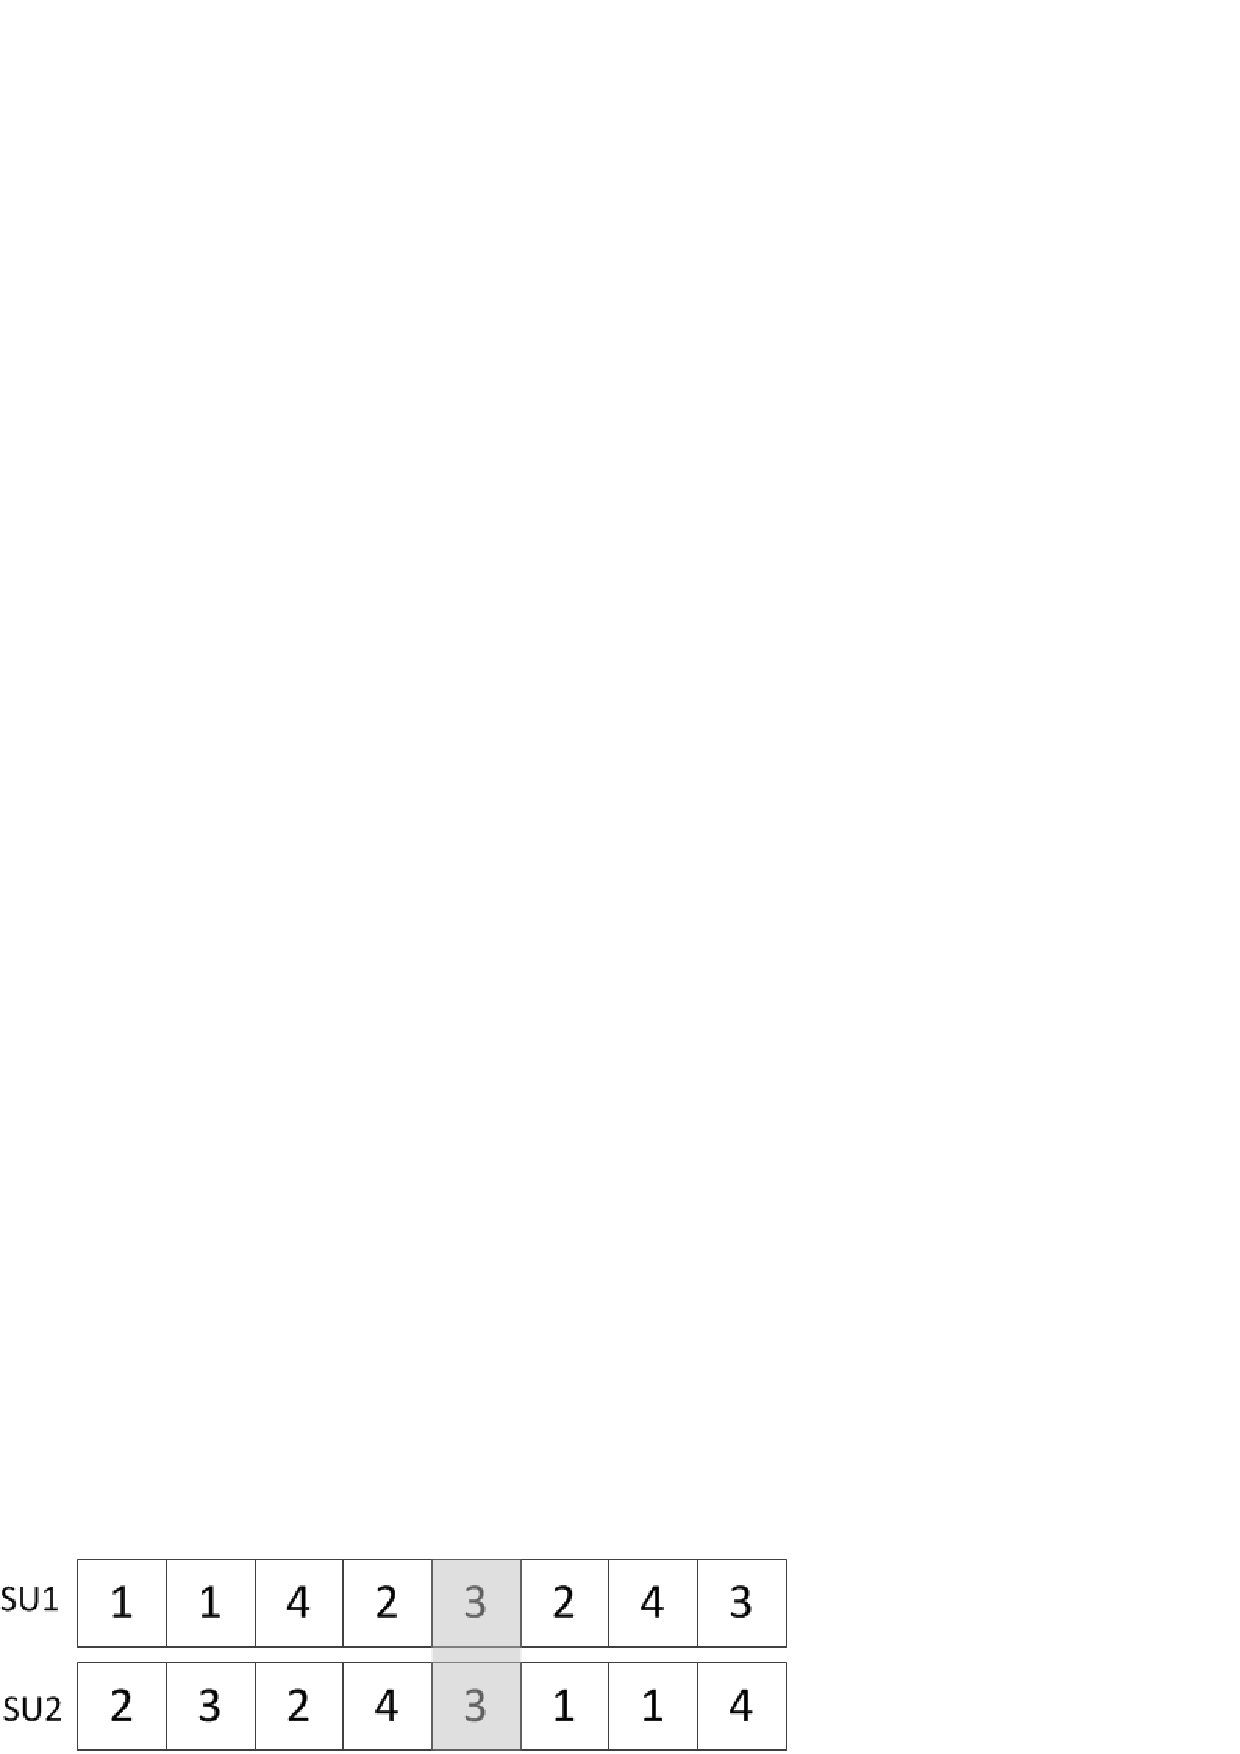
\includegraphics[width=10cm,height=2.5cm]{sec_1_2_rend0.jpg} 
        \caption{An example of a successful rendezvous process.} 
        \label{1_2_example} 
    \end{center} 
\end{figure}

 In order to evaluate
a rendezvous scheme, three performance metrics are defined  \cite{hLiu12TACOR}:
\textit{TTR}, \textit{MTTR}, and \textit{ETTR}, where \textit{TTR} is the
time to rendezvous from the moment the channel hopping starts until the moment
two SUs meet on a common available channel, \textit{MTTR} is the maximum
possible time required to have a successful rendezvous, and \textit{ETTR}
is the expectation of the time to a successful rendezvous.
  
\section{Wide-band Cognitive Radio Networks}
The original purpose of cognitive radio is to improve the utilization of the spectrum which has been allocated. However, according to the FCC, the allocated spectrum, ranging from $3$KHz to $300$GHz, is very wide. Though we cannot expect cognitive radio to work in that wide spectrum, the number of channels a cognitive radio can access may be hundreds or thousands.  For instance, according to \cite{cCordeiro05IEEE80222P}, the TV band which can be utilized by SUs is from $54$MHz to $862$MHz and the bandwidth of each channel is $6$MHz. This corresponds to a total of $134$ channels. With the increase of the number of channels in a CRN, the time for an SU to sense the whole band and the energy consumed in the sensing process will increase. In \cite{aGiannoulis13MAOWS}, the importance of considering the wide-band scenario is explored and a scheme for mobile access of wide-band networks is proposed. However, to the best of our knowledge, there are no existing papers which can efficiently solve the communication problems in CRNs coming from the wide-band spectrum without a (common control channel) CCC.  Therefore, addressing the communication problems stemming from the wide-band spectrum is necessary.

In \cite{hLiu10RWBCH, cXin11PAOAC, nTheis11RFCR, zLin11JSBCH, yZhang11ETCH, ySong12ADBPI, rGandhi12FRFMC, romaszko2012quorum, bian2009quorum, jShin10ACRSF}, several rendezvous schemes for CRNs are proposed. However, these schemes only focus on the rendezvous problem itself while ignoring the following practical communication scenarios in wide-band CRNs. First, they do not consider the wide-band scenario. All of them just consider that there are only a small number of channels (at most tens of channels) in the network and SUs will utilize all the channels to design the channel hopping sequence and perform channel hopping, while there may be hundreds of channels for a CRN.  As the number of channels increases, the time to sense all the channels to get available channels and to rendezvous  will increase significantly, according to the results shown in \cite{hLiu12TACOR}. Second, they do not consider the scenario that time slots of two SUs are not perfectly aligned which may make a rendezvous unsuccessful, and the optimal time slot length to guarantee a successful rendezvous. Thus, a practical communication framework for  wide-band CRNs without a CCC that  can address the above problems is needed.

\section{Rendezvous Schemes Without Predetermined Sender and Receiver}
The past works in rendezvous only consider how to make two or multiple SUs rendezvous on a common available channel within bounded time slots, which is defined as the \textit{channel rendezvous} problem in this research. However, the process of sending or receiving RTS or CTS packets  is not considered. Past rendezvous schemes implicitly require a sender-and-receiver relation between the two rendezvous SUs, i.e.,  an SU sender always sends an RTS packet on each of its hopped channels during each time slot, while the other SU always listens on each of its hopped channels. If the other SU receives an RTS packet, it replies a CTS packet to set up a link with the SU sender. However, during the initialization phase of a CRN, every SU tries to rendezvous with other SUs to exchange their control information. There is no explicit sender or receiver role such that an SU is always a sender or receiver, since it cannot know if other SUs are sending or waiting for RTS packets. Therefore, for a SU, whether tuning its half-duplex radio to the sending or receiving mode during a time slot is a problem, which is defined as the \textit{send-or-receive problem} in this research.

This \textit{send-or-receive problem}  is a practical problem when each SU is equipped with multiple cognitive radios or a single radio. For an SU equipped with a single radio, it can only be a sender or receiver during a time slot. When considering multiple radios, an SU can be a sender and receiver simultaneously by assigning sending or receiving tasks to different radios. Past rendezvous schemes considering multiple cognitive radios only focus on the \textit{channel rendezvous} between two radios of two SUs \cite{lYu13MREFR}. They define a successful rendezvous between two SUs when any two radios of the two SUs hop to a common available channel at the same time slot. However, there also exists the \textit{send-or-receive problem} for the two multiple-radio SUs. Therefore, when considering multiple-radio rendezvous, how to assign a sending or receiving task to each radio is a problem which has never been addressed in previous rendezvous schemes.

\section{Rendezvous Process Considering Directional Antennas}
Previous works in rendezvous only consider how to let two or multiple SUs rendezvous on a common available channel within a  bounded time, when SUs are equipped with omni-directional antennas. However, omni-directional antennas may cause interference to all the PUs within the entire transmission area of an SU simultaneously, since omni-directional antennas transmit towards all directions. Especially, if the distance between two SUs increases, in order to keep them connected, the SUs increase their transmission power. As a result, the transmission range of an SU increases, which will cause interference to more PUs. Even though previous rendezvous schemes assume that during each time slot, an SU should first sense a channel before accessing it, PUs can still return to that channel during the transmission period of an SU as PUs' traffic is unknown to SUs. Therefore, in a CRN, we should try to decrease the number of PUs who could potentially be interfered by a SU's rendezvous process.

One way to overcome the above problem is to equip each SU a directional antenna. With a directional antenna, an SU can transmit toward a specific direction with a certain angle. The area covered by the signals from a directional antenna is called a \textit{transmission sector}. Therefore, an SU with a directional antenna can only cause interference to PUs within its transmission sector rather than the whole transmission area during each time slot. Another benefit of the directional antenna is that after a successful rendezvous, two SUs can know each other's location. For the data transmission or the next rendezvous process, two SUs can just tune their directional antennas to the transmission sectors which can cover each other.

However, the blind rendezvous problem with directional antennas has not been considered in the literature yet. In this research, we propose fully distributed rendezvous schemes for SUs equipped with directional antennas. We first propose a new rendezvous problem called the \textit{sector rendezvous problem} between two SUs. For a sector rendezvous process, there exist the \textit{indexing problem} and \textit{sector number} problem that make the sector rendezvous problem different from the existing channel rendezvous problem. We cannot directly apply existing channel hopping sequences in \cite{nTheis11RFCR, zLin11JSBCH, yZhang11ETCH, rGandhi12FRFMC, zG13NOABR, jLi14ANCFF, ySong14AQBBP, hLiu12JSRAF, ySong15BRACER} to the sector rendezvous problem since they do not consider the indexing problem and assume that each SU can access the same number of channels. In order to tackle the sector rendezvous problem, we design fully distributed sector rendezvous schemes for an SU only based on the SU's own information. Our proposed schemes can guarantee successful sector rendezvous and channel rendezvous simultaneously within a bounded time. The proposed sector rendezvous schemes can work on top of any existing channel hopping scheme which  guarantees a successful channel rendezvous within a bounded time.

\section{Power Control to Maximize the Number of Common Available Channels}
The available channels of an SU are critical  
for its transmission because with more available channels, the SU can have more channel  
sources to choose. Moreover, in a CRN, it is necessary for two SUs to rendezvous on  
the same available channel to communicate with each other. More common available  
channels also mean more opportunities for the two SUs to meet on the same channel.  
Therefore, the most important factor for an SU communicating pair is their common  
available channels rather than their own available channels. In CRNs, the number  
of the common available channels plays an important role in many network  
operations such as channel rendezvous, spectrum handoff, and broadcast.  
  
In CRNs, in order to know which channels are available currently,  an SU has to sense the spectrum. The sensing range of an SU is the range within  which the SU can sense the channels occupied by PUs. Thus, the sensing range  determines the available channels of a SU. The larger the sensing range, the more unavailable channels that could be sensed by a SU. Now, the issue is how to determine the sensing ranges of an SU sender and SU receiver in order to get a maximum number of common available channels? However, none of the existing papers in rendezvous or spectrum handoff consider improving the performance by increasing the number of available  
channels, especially the common available channels between two SUs in CRNs.  
In this research, we first illustrate the relationship among the number of common available  channels, SU transmission power, sensing threshold, and sensing range of an SU sender and  receiver. Then, we propose a power control protocol to maximize the number of common  available channels between two SUs in CRNs. Our proposed protocol is practical and  easy to implement.

\section{Overview of the Proposed Rendezvous Schemes and Spectrum Management for CRNs}
Fig. \ref{fig:research_overview} shows the overview of our proposed Research.
In order to achieve efficient rendezvous and spectrum management in CRNs, we first propose a rendezvous framework for wide-band cognitive radio networks considering hundreds of channels. In this framework, we first propose a spectrum split scheme to split the wide-band spectrum into several spectrum segments and map each SU to a specific spectrum segment. Next, we propose an efficient rendezvous scheme specific for this framework considering spectrum splitting which enables two SUs to reach a fast and successful rendezvous. In the designed framework, we assume that a CCC is not required, there is not a central controller or base station for information exchange, and each SU does not know any information about the other SU before they achieve a successful rendezvous. All these assumptions are very practical concerning the characteristics and limitations of cognitive radio networks.
\begin{figure}[hbtp] 
    \begin{center} 
        \includegraphics[width=12cm,height=8cm]{sec_1_7_ResearchOverview1.jpg} 
        \caption{Overview of the proposed research} 
        \label{fig:research_overview}
    \end{center}  
\end{figure} 

Next, we propose two efficient rendezvous schemes under the scenarios that there is not a predetermined sender or receiver for a rendezvous process during the initialization phase of cognitive radio networks, which is very practical. Under this scenario, we define a new type of rendezvous called \textit{link rendezvous}. In order to design the rendezvous schemes to achieve successful  link rendezvous, we designed two innovative spectrum management schemes called \textit{channel group} and \textit{virtual channels}. In the proposed rendezvous schemes, we also assume each SU do not know any control information about the other SUs, which is very practical.

Moreover, we propose an efficient rendezvous scheme specific for  SUs which are equipped directional antennas. Under this scenario, the rendezvous process could be more completed since each SU could be equipped with heterogeneous directional antenna and it does not know any information about the other SUs. We define a new type of rendezvous called \textit{sector rendezvous} when considering directional antennas. Our propose rendezvous scheme can efficiently solve the sector rendezvous problem under practical scenarios.

Last, we propose a power control protocol which can maximize the number of common available channels between two SUs. Common available channels between two SUs are critical in achieving a successful rendezvous and spectrum handoff. In the proposed scheme, after two SUs successfully  achieve a  rendezvous, they first exchange some control information, based on which they could  perform distributed power control  to maximize the number of common available channels, which could improve the performance of their next rendezvous or spectrum handoff process.
% 
% 
% \section{Proposal Organization}
% The rest of this proposal is organized as follows. In Chapter \ref{char:RW}, %the related works in CRNs are introduced. In Chapter \ref{char:PR}, five %schemes are proposed regarding practical problems for the rendezvous process %in CRNs. We conclude our research, address our future works, and list publications %in Chapter \ref{char:conclusion}.

\chapter{RELATED WORK}
\label{char:RW}
\section{Existing Protocols for Information Exchange in CRNs}
The initialization of a CRN is critical, because each SU may not know any
information about other SUs in the same network before information exchange.
However, due to the dynamic characteristics of CRNs, obtaining the basic
but time-varying control information, such as the available channel sets
and locations, of SUs is very challenging. For simplicity, many existing
papers address this challenge by assuming the existence of a common control
channel (CCC) in the network and using the CCC for all control information
exchange \cite{cCordeiro05IEEE80222P, jJia08HCMAC, vBrik05DSAP}. However,
a CCC may suffer the following problems. First, a CCC may not be available
simultaneously to all the SUs in a  network. Second, even though a CCC exists,
due to the dynamics of CRNs, its availability over the time is subject to
 PUs' traffic. Third, a single CCC in a network may suffer the congestion
problem and is fragile under  attacks. In order to overcome these drawbacks,
some schemes are proposed to form several SU clusters in a network and choose
a common available  channel as the CCC in each cluster \cite{mKim09DCPFC,lLazos09SOBCC}.
However, in order to form a cluster, each SU has to know certain information
about its neighboring SUs, which is also not practical for a CRN without
any control information exchange before the initialization. Rather than deploying a CCC which is not practical for a CRN, single rendezvous coordination schemes and multiple rendezvous coordination schemes were proposed to realize imformation exchange between SUs in \cite{ySong10CHBPS, ySong12APSHF, jMo08COMMP, hSoMcMAC}. However, for single rendezvous coordination schemes, all the SUs should follow the same channel hopping sequence which requires strict synchronization between SUs; for  multiple rendezvous coordination schemes, each SU should know the channel hopping sequence of its communicating peer which is also not practical considering distributed scenarios. Moreover, all those protocols did not consider the wide-band scenario, which may cause serious delay during the information exchange process. Another promising technology for information exchange is to implement practical broadcasting protocols in CRNs. In \cite{yKon08SBiMCRN, arachchige2011minimal, ySong11AQBPF, ySong12ADBPI} several broadcasting protocols are proposed. However, in \cite{yKon08SBiMCRN, arachchige2011minimal}, some critical information like the channel availability and network topology are assumed to known for all the SUs, which is not practical considering distributed scenarios. A CCC is required in \cite{ySong11AQBPF} to achieve a Quality-of-Service (QoS) based protocol. In addition, a broadcast protocol under blind information is proposed in \cite{ySong12ADBPI}. However, the rendezvous scheme in this protocol cannot guarantee a successful rendezvous and it also did not consider the wide-band scenario.

\section{Existing Distributed Channel Hopping Schemes}
Another more practical method for setting up a link between a SU pair is
to implement a distributed channel hopping scheme. In this scheme, a time-slotted system
is deployed, and during each time slot, each SU hops to a channel based on
a designed channel hopping sequence. Once two SUs hop to the same channel
which is available to both of them simultaneously, they could set up a link
on this channel through an RTS/CTS (Request-to-Send / Clear-to-Send) exchange.
This is called the \textit{blind rendezvous} process for a CRN during which
the two SUs do not have any information about each other before a successful
rendezvous. Past works on blind rendezvous mainly focus on designing well
performed channel hopping sequences and channel hopping schemes which can
guarantee a successful rendezvous within a bounded time.

In \cite{hLiu10RWBCH, cXin11PAOAC, zLin11JSBCH, yZhang11ETCH, ySong12ADBPI, rGandhi12FRFMC, romaszko2012quorum, jShin10ACRSF, ySong14AQBBP, hLiu12JSRAF, ySong15BRACER, zG13NOABR, xLiu14APSARP, sWu14RFHSD, tWu14CACH}, several rendezvous schemes for CRNs are proposed. However, these schemes only focus on the rendezvous problem itself or designing efficient channel hopping sequences, while ignoring the following practical communication scenarios in wide-band CRNs. First, they do not consider the wide-band scenario. All of them just consider that there are only a small number of channels (at most tens of channels) in the network and SUs will utilize all the channels to design the channel hopping sequence and perform channel hopping, while there may be hundreds of channels for a CRN.  As the number of channels increases, the time to sense all the channels to get available channels and to rendezvous  will increase significantly, according to the results shown in \cite{bian2009quorum, hLiu12TACOR, nTheis11RFCR}. Second, the process of sending or receiving RTS or CTS packets  is not considered. Past rendezvous schemes implicitly require a sender-and-receiver relation between the two rendezvous SUs, i.e.,  an SU sender always sends an RTS packet on each of its hopped channels during each time slot, while the other SU always listens on each of its hopped channels. If the other SU receives an RTS packet, it replies a CTS packet to set up a link with the SU sender. However, during the initialization phase of a CRN, every SU tries to rendezvous with other SUs to exchange their control information. There is no explicit sender or receiver role such that an SU is always a sender or receiver, since it cannot know if other SUs are sending or waiting for RTS packets. Third, they cannot directly apply to the rendezvous problem considering directional antennas since they do not consider the indexing problem and assume that each SU can access the same number of channels. 

\section{Existing Schemes Considering Common Available Channels and Power Control}
Common available channels play an important role in CRNs since any SU pair can only establish communicating links through them. However, two SUs cannot determine any common available channel before information exchange or there is not a common control channel (CCC) in a CRN.
Many existing papers in CRNs have proposed different algorithms for rendezvous, broadcast, and spectrum handoff by directly using the common available channels of SUs. Serveral random  channel selection schemes were proposed in \cite{cXin11PAOAC, cXin11AAORS, cXin10ORDSA} to make sure two users can  rendezvous on the common available channel. However, those schemes cannot guarantee a successful rendezvous as long as there is a common available channel between two SUs. Rendezvous among multiple SUs in \cite{ySong12APSHF} is realized by generating the same channel hopping sequence or each SU should know the channel hopping sequence of each other, which is not practical considering distributed scenarios.  Blind rendezvous schemes based on common available channels and channel hopping are proposed in \cite{hLiu10RWBCH, cXin11PAOAC,  zLin11JSBCH, yZhang11ETCH, lJiao09ASRBC, jJia13RPBOM, zLin13EJSRA, rPaul14MRISCR, lYu13MREFR}. However, they did not consider how to optimize the number of common available channels which could improve the performance of a rendezvous scheme according to the analysis in them. In addition, distributed algorithms are proposed in \cite{ySong10CHBPS, ySong12APSHF} to avoid collisions during a spectrum handoff based on the common available channels between two SUs. An optimal channel selection sequence for the two SUs after each spectrum handoff process  is designed in 
\cite{lWang12OTCSD, lWang12MAAFS}. Moreover, multiple distributed broadcast schemes based on the common available
channels  between two users are proposed in 
\cite{ySong12ADBPI, ySong11AQBPF, ySong14AQBBP, ySong15BRACER}. However, all these papers just directly utilize the common available channels while ignoring how to maximize the number of common available channels. 

Power control is an effective way to improve the performance of a CRN by optimizing the utilization of physical links between SUs. In \cite{ySong09optimal}, a power control protocol was proposed to maximize the concurrent transmission region of a CR transmitter to maximize throughput without causing harmful interference to PUs. Price-based power control algorithms were proposed in \cite{wang2013anovel, wang2014optimal} to maximize the revenue of both base stations and SUs by modeling games among base stations and SUs. \cite{parsaeefard2013robust} proposed a robust distributed power allocation algorithm for uplink to maximizing the social utility of SUs when channel gains from SUs to primary base stations and interference caused by PUs to SUs' base station are uncertain. \cite{dall2011power, sorooshyari2012power} proposed some power control algorithms to optimize the channel utility and networking throughput in CRNs. In \cite{li2011anewgame, xiao2011asimple, zhou2012reinforcement}, several games were modeled to optimize the networking performance considering the problem of interference between SUs and PUs. However, all the these papers only consider utilizing power control to optimize the physical layer of CRNs rather than the common available channels for the MAC layer. In addition, in order to model a game or optimization problem, a common control channel (CCC) is required for information exchange which is not practical considering distributed scenarios.

\chapter{Communication Framework for Wide-band Cognitive Radio Networks}
\label{chapter_wide_band}
In this chapter, we first propose a rendezvous framework for wide-band cognitive radio networks
considering hundreds of channels. In this framework, we first propose a spectrum
split scheme to split the wide-band spectrum into several spectrum segments
and map each SU to a specific spectrum segment. Next, we propose an efficient
rendezvous scheme specific for this framework considering spectrum splitting
which enables two SUs to reach a fast and successful rendezvous.
\section{System Model}
\label{sec_3_1_sys}
We consider that SUs in a CRN can dynamically access a  wide-band spectrum which has a total of $M$ channels indexed from $1$ to $M$, where $M$ is a large number which could be hundreds. There are totally $N$ SUs. Each SU is equipped with only one cognitive radio that cannot perform spectrum sensing and data transmission at the same time. Each SU has a unique ID which can be a  positive integer. Furthermore, we assume that each SU can obtain its available channel set  using a spectrum sensing algorithm \cite{iAkyildiz06NGDSA}. Initially, an SU does not know any information about other SUs, even their unique IDs. A  time-slotted system is adopted in this CRN. In each time slot, an SU either hops onto a channel according to its hopping sequence or stays on its current channel to continue the current communication with another SU. Time slots of different SUs are not necessarily synchronized, which is practical and easy to implement. SUs in the CRN attempt to get  information about other SUs within its transmission range, send packets to other SUs, or receive packets from other SUs. 

In the rest of the section, we consider the following two scenarios concerning the available channel sets of an SU pair.

\textit{Symmetrical model}: Any SU pair has exactly the same available channel set. According to  \cite{ySong14AQBBP, ySong11AQBPF, ySong15BRACER}, the similarity of the available channel sets between two SUs within one hop is over $85\%$. Thus, this model is reasonable. Moreover, studying this scenario can help us to get solutions for more complicated scenarios.

\textit{Asymmetrical model}: Any SU pair may have different but overlapping available channel sets. This scenario is more practical because of the dynamics caused by PUs' and SUs' traffic and locations.

%Add a new paragraph to define asym/sym model and MTTR ETTR .
\section{The Proposed Framework}
\label{sec:framework}
The goal of our proposed framework is to design efficient distributed schemes for each SU to guarantee that it can communicate with other SUs successfully in a wide-band CRN. The framework mainly contains three parts: the initialization process, the process to get control information from neighboring SUs, and the process to send packets to a specific SU. Moreover, the framework does not require a common control channel (CCC) for information exchange. The flow charts of these three parts are shown in Fig. \ref{fig:frame}.
\begin{figure}[hbtp] 
    \begin{center} 
        \includegraphics[width=8cm,height=8cm]{sec_3_1_frame.jpg} 
        \caption{The flow charts of our proposed framework.} 
        \label{fig:frame}
    \end{center}  
\end{figure} 

During the initialization process, each SU first divides the whole wide-band spectrum into several virtual spectrum segments (SS). Based on \textbf{Algorithm \ref{al:spl}} (which is explained in Section \ref{sec:split}), each SU can get a unique list containing the number of channels in each SS. We call it the spectrum splitting list (SSL). Using the unique SSL, an SU can obtain the channel index of the start and end channel in each SS (shown in \textbf{Algorithm \ref{al:id}}). Then, each SU  uses its ID (based on \textbf{Algorithm \ref{al:id}}) to determine its home spectrum segment (HS). \textbf{Algorithm \ref{al:id}} is based on mapping all the SUs evenly to the whole spectrum, where we assume that the IDs of SUs are evenly distributed within a certain range. An SU  hops from a channel to another according to the designed channel hopping sequence (based on \textbf{Algorithm \ref{sec_3_1_algorithm_generate}} which is explained in Section \ref{sec:seq}) within its HS. Since  SUs are not synchronized, they may be at different positions of the same hopping sequence even they locate in the same HS. This is the initialization process of an SU who just starts in a CRN, as shown in the left of Fig. \ref{fig:frame}.
\begin{algorithm} 
  \caption{The algorithm to determine a SU's home spectrum's index}
  \begin{algorithmic}[1] 
  \label{al:id}
   \REQUIRE ~~\\ 
    The SU's ID $x$.\\
    \ENSURE ~~\\
     The SU's home spectrum's index;
    \STATE Use \textbf{Algorithm \ref{al:spl}} to get the SSL $l$;\\
    \STATE $y = (x-1) \% M+ 1$; //The channel index starts from 1\\
    \STATE $sum=0$;\\
    \FOR{$i=0$ to $l.length-1$}
        \IF{$y > sum\ \mbox{and}\ y \leq sum + l[i]$}
                    \RETURN $i$;\\
                \ENDIF
                \STATE $sum += l[i]$;\\
    \ENDFOR
  \end{algorithmic} 
\end{algorithm}

After the initialization process, an SU  tries to get the control information of all its neighboring SUs which are hopping in the same or different spectrum segments (SSs). We assume that when an SU is not transmitting data packets, it first performs \textbf{Algorithm \ref{al:sym}} or \textbf{Algorithm \ref{al:asym}} (which is explained in Section \ref{sec:seq}) to rendezvous with an SU in its home spectrum segment (HS) and exchange all their known control information about themselves and others. Through this process, each SU can get all the other SUs' information within the same SS and exchange all of their known information. Therefore, after rendezvous and exchange control information with one existing SU in a SS, a  SU can get the control information of all the other SUs in that SS, and all the existing SUs in the SS can also get the information of this SU and all its known information about other SUs. Then, the SU can sequentially hop to each SS, rendezvous with one SU in that SS, and exchange all the  known control information about other SUs by executing \textbf{Algorithm \ref{al:sym}} or \textbf{Algorithm \ref{al:asym}}.  The SU will hop to a next SS only when it has rendezvoused with an SU in the current SS or the time spent in the current SS has already been more than the MTTR of the applied rendezvous scheme (there are no SUs in current SS) . Finally, the  SU will obtain  and update the control information of all other  SUs in the network. An SU can perform the above process periodically to update the control information about other SUs and inform its own change due to the dynamic characteristics of CRNs. The process of getting  the control information of all the neighboring SUs is shown in the middle of Fig. \ref{fig:frame}. 

After the above process of control information exchange, an SU will get some information about other SUs such as their IDs. When an SU wants to send packets to a specific SU, it first uses the receiver's ID  to determine the receiver's home spectrum segment (HS)  (based on \textbf{Algorithm 1}). Then, the SU sender  executes \textbf{Algorithm \ref{al:sym}} or \textbf{Algorithm \ref{al:asym}} to realize rendezvous with the SU receiver in the SU receiver's HS for communications. The flow charts of  communicating with a specific SU is shown in the right of  Fig. \ref{fig:frame}. Because of the spectrum splitting design, the time to obtain control information and to set up communications can be significantly reduced since an SU pair only needs to rendezvous within a specific spectrum segment (SS). In addition, the probability that multiple pairs of SUs rendezvous on the same channel is also reduced since different pairs of SUs may rendezvous in different spectrum segments (SSs). In the following sections, we will give the details of the proposed algorithms in our framework.

\section{Proposed Rendezvous Schemes Under the Symmetrical Model}
\label{sec:seq}
An SU sender and receiver have exactly the same available channel set under the symmetrical model. This may not be very practical. However, the algorithms developed under this model are the basis for the asymmetrical  model. 
%\subsubsection{Hopping Sequence Design}

 Under this scenario, each SU has the same available channels in each SS. Each SU hops within its HS according to a channel hopping sequence generated based on its available channel set. Assume that the number of the available channels of both the SU sender and receiver in the SU receiver's HS is $n$. Since an SU sender and receiver have the same available channel set, we use the indexes of all the available channels in a SS, assuming to be from $1$ to $n$, to design the channel hopping sequence. We desire to get a target sequence $s = {s_{1}s_{2}\dots s_{2n}}$ whose length is $2n$ and each channel index from $1$ to $n$  appears exactly twice in $s$. When an SU sender wants to rendezvous with an SU receiver, it first hops to the HS of the SU receiver, generates the same channel hopping sequence as the SU receiver's, and then starts to hop on channel $s_{1}$. Both the SU sender and receiver hop according to the sequence sequentially and circularly, which means that when an SU reaches the end of the hopping sequence, it will continue to hop onto the first channel of the sequence in the next time slot. Assume that the SU receiver is initially on channel $s_{c}, 1\leq c \leq 2n$. We denote $\varepsilon$ as the distance between the SU sender and SU receiver on the channel hopping sequence due to the asynchronization. Therefore, $\varepsilon = c-1$ or $\varepsilon = 2n-(c-1)$ when considering the circulation of the channel hopping sequence. We define the rendezvous sequence (RS) as follows:

\textit{Rendezvous Sequence (RS)}: The sequence $s$ is a RS when no matter what $\varepsilon$ is, within $2n-1$ time slots, the SU sender and receiver will hop on a same channel if both of them hop according to the same hopping sequence sequentially and circularly.

 We use $s$ to represent our desired rendezvous sequence for the rest of the section.  
We induce  the following lemma to help us design our rendezvous sequence. 
\begin{lemma}
\label{lemma:guar_rend}
Assume that $s_{i} = s_{j} = k, i < j$, $1\leq k\leq n$. If $j - i = k$, $s$ could be a RS.

\end{lemma}
\begin{proof}
We define the \textit{Sequential Distance} of  the element $k$ in the sequence $s$ as $ d_{k} = j-i=k$, and the  \textit{Circular Distance} of  the element $k$ in the sequence $s$ as $ D_{k} = 2n+i-j=2n-k$, which is the number of time slots taken to hop from $s_{j}$ to $s_{i}$ circularly in $s$. We define the distance pair of the channel index $k$ as $p_{k} = (d_{k}, D_{k})$. Since each $d_{k}$ is different and bounded in $[1,n]$ and each $D_{k}=2n-d_{k}$ is different and bounded in $[n,2n-1]$, each $p_{k}$ is different. Assume that initially the SU sender is on channel $s_{1}$ and the SU receiver is on channel $s_{c}$ Therefore, $\varepsilon=c-1$ or $\varepsilon = 2n-(c-1)$, where $0\leq \varepsilon \leq 2n-1$. We ignore the case when $\varepsilon=0$, because under this case, the two SUs are already on the same channel. Thus, we only need to prove our lemma when $1\leq \varepsilon \leq 2n-1$. Since each $p_{i}$ is different, we can definitely find a $p_{t}$ such that $\varepsilon = d_{t}\ \mbox{or}\ D_{t}$. Suppose $s_{i1} = s_{j1} = t, i1 < j1$. Thus, when the SU sender hops on channel $s_{i1}$, it will rendezvous with the SU receiver on channel $s_{j1}$, or when the SU sender hops on channel $s_{j1}$, it will rendezvous with the SU receiver on channel $s_{i1}$. Therefore, sequence $s$ can guarantee a successful rendezvous within $2n-1$ time slots no matter which channel the SU receiver dwells on at the beginning of the rendezvous process.
\end{proof}

In order to efficiently generate $s$, we notice that $s$ has the following properties. 
\begin{lemma}
\label{lemma:no_exist}
When $n = 4t+2$ or $4t+3$, where $t$ is an integer and $t \geq 1$, the rendezvous sequence does not exist.
\end{lemma}
        \begin{proof}
        Designing a rendezvous sequence $s$ as described in \textbf{Lemma \ref{lemma:guar_rend}} is equivalent to dividing  $1,2,\dots, 2n$,  these $2n$ numbers into two lists $l_{l}$ and $l_{r}$, each of which has exactly $n$ different numbers, such that for $k=1,2,\dots,n$, $l_{r}[k] - l_{l}[k] = k$. Then, we have
        \begin{equation}
        \label{sec_3_1_eq_sum1}
        \sum^{n}_{k=1}l_{r}[k]-\sum^{n}_{k=1}l_{l}[k]=\sum^{n}_{k=1}k=\DF{n(n+1)}{2},
        \end{equation}
        \begin{equation}
        \label{sec_3_1_eq_sum2}
        \sum^{n}_{k=1}l_{r}[k]+\sum^{n}_{k=1}l_{l}[k]=\sum^{2n}_{k=1}k=n(2n+1).
        \end{equation}
        Combining \eqref{sec_3_1_eq_sum1} and \eqref{sec_3_1_eq_sum2}, we can get 
        \begin{equation}
        \label{sec_3_1_eq_sum3}
        \sum^{n}_{k=1}l_{r}[k]=\DF{5n^{2}+3n}{4}.
        \end{equation}
        When $n=4t+2$ or $4t+3$,where $t$ is an integer and $t \geq 1$, the right-hand side of \eqref{sec_3_1_eq_sum3} is not an integer which contradicts the fact that it is a sum of $n$ integers.
        \end{proof}
\begin{lemma}
\label{sec_3_1_lemma_exist}
When $n=4t$ or $4t+1$, where $t$ is an integer and $t \geq 1$, the rendezvous sequence always exists.
\end{lemma}
        \begin{proof}
        When $n=4$, sequence $"1,1,4,2,3,2,4,3"$ satisfies the requirements of our desired rendezvous sequence.
        When $n=5$, sequence $"1,1,5,2,4,2,3,5,4,3"$ satisfies the requirements of our desired rendezvous sequence.
        When $n > 5$, the proof can be found in the second page of \cite{tSkolem57OCDOI}.
        \end{proof}
Based on the proof of \textbf{ Lemma \ref{lemma:no_exist}} and \textbf{ Lemma \ref{sec_3_1_lemma_exist}}, we propose \textbf{Algorithm \ref{sec_3_1_algorithm_generate}} to generate our desired rendezvous sequence. Using the channel hopping sequence generated based on \textbf{Algorithm \ref{sec_3_1_algorithm_generate}} and \textbf{Lemma \ref{lemma:guar_rend}}, we design the rendezvous algorithm under the symmetrical model as shown in \textbf{Algorithm \ref{al:sym}}.
%\renewcommand\baselinestretch{0.8}\selectfont 
\begin{algorithm} 
  \caption{The algorithm to generate a rendezvous sequence}
  \begin{algorithmic}[1] 
  \label{sec_3_1_algorithm_generate}
    \REQUIRE ~~\\
    The number of channels to generate the channel hopping sequence: $n$
    \ENSURE ~~\\
    The desired rendezvous sequence: $s$\\
    \IF{$n<4\ \mbox{or}\ n\%4==2\ \mbox{or}\ n\%4==3$}
                \STATE $s=\phi$;
                \RETURN $s$;
        \ENDIF
    \IF{$n==4$}
                \STATE $s=[1,1,4,2,3,2,4,3]$;
                \RETURN $s$;
        \ENDIF
        \IF{$n==5$}
                \STATE $s=[1,1,5,2,4,2,3,5,4,3]$;
                \RETURN $s$;
        \ENDIF
        \STATE Let $pl=\phi$ be the list of all the position pairs;
        \STATE $m=\lfloor n/4 \rfloor$;
        \IF{$n > 4\ \mbox{and}\ n\%4==0$}
                \STATE Add all pairs $(4m+r, 8m-r)$, for $r=0,1,\dots,2m-1$, to $pl$;
                \STATE Add pairs $(2m+1, 6m)$ and $(2m, 4m-1)$ to $pl$;
                \STATE Add all pairs $(r, 4m-1-r)$, for $r=1,3,\dots,m-1$, to $pl$;
                \STATE Add pair $(m, m+1)$ to $pl$;
                \STATE Add all pairs $(m+2+r, 3m-1-r)$, for $r=0,1,\dots,m-3$, to $pl$;
        \ENDIF
        \IF{$n > 4\ \mbox{and}\ n\%4==1$}
                \STATE Add all pairs $(4m+2+r, 8m+2-r)$, for $r=0,1,\dots,2m-1$, to $pl$;
                \STATE Add pairs $(2m+1 ,6m+2)$ and $(2m+2, 4m+1)$ to $pl$;
                \STATE Add all pairs $(r, 4m+1-r)$, for $r=1,3,\dots,m$, to $pl$;
                \STATE Add pair $(m+1, m+2)$ to $pl$;
                \STATE Add all pairs $(m+2+r, 3m+1-r)$, for $r=1,2,\dots,m-2$, to $pl$;
        \ENDIF
        \FOR{$i=1$ to $n$}
                \STATE $s[pl[i].first] = s[pl[i].second] = pl[i].second - pl[i].first$;
        \ENDFOR
        \RETURN $s$;
  \end{algorithmic} 
\end{algorithm} 
%\renewcommand\baselinestretch{0.8}\selectfont 
\begin{algorithm} 
  \caption{The rendezvous algorithm for an SU sender under the symmetrical model}
  \begin{algorithmic}[1] 
  \label{al:sym}
    \REQUIRE ~~\\ 
    The available channel set $C$ of the SU sender within the SU sender's HS.\\
    \STATE $n$ equals the size of $C$;\\
    \IF{$n\%4==2$ or $n\%4==3$}
                \STATE $m = 4(\lfloor n/4 \rfloor+1)$;\ \ /* To guarantee the existence of the RS */\\
        \ELSE
                \STATE $m = n$;\\
        \ENDIF
    \STATE Generate the channel hopping sequence $s$ based on $m$ and \textbf{Algorithm \ref{sec_3_1_algorithm_generate}};\\
    \FOR{$k=1$ to $2m$}
                \IF{$s_{k} > n$}
                        \STATE $s_{k} = s_{k} \% n$;\ \ /* To guarantee $s_{k}$ to be within $n$ */\\
                \ENDIF
        \ENDFOR
    \STATE $i = 1$;\\
    \FOR{$j = 1$ to $2m-1$}
             \IF{The sender receives a CTS packet on channel $C_{s_{i}}$ of the receiver's HS}
             \STATE Perform communications;\\
        \ELSE
              \STATE $i++$;\\
       \ENDIF
    \ENDFOR
  \end{algorithmic} 
\end{algorithm}

We define a round of  channel hopping as  the length of the $2n$ time slots an SU hops sequentially and circularly  according to the channel hopping sequence. An example of rendezvous in one channel hopping round under the symmetrical model is shown in Fig. \ref{fig:sys_ren}. We assume that the number of available channels of an SU pair is $4$. We label each available channel using the index from $1$ to $4$.  Based on \textbf{Algorithm \ref{sec_3_1_algorithm_generate}}, their channel hopping sequence is $"1,1,4,2,3,2,4,3"$. Assume that the SU sender starts hopping from the channel  whose index is $s_{1}=1$ and the SU receiver currently stays on the channel whose index is $s_{3}=4$. Then, the SU sender and receiver will rendezvous on the channel whose index is $s_{4}=2$ after $3$ time slots.
\begin{figure}[hbtp] 
    \begin{center} 
        \includegraphics[width=12cm,height=4cm]{sec_3_1_sys.jpg} 
        \caption{An example of rendezvous under the symmetrical model.} 
        \label{fig:sys_ren} 
    \end{center} 
\end{figure} 

From \textbf{Lemma \ref{lemma:guar_rend}} and \textbf{Algorithm \ref{al:sym}}, we can induce \textbf{Theorem \ref{theo:ettr}}.
\addtocounter{theorem}{-3}
        \begin{theorem}
        \label{theo:ettr}
        Under the symmetrical model, \textbf{Algorithm \ref{al:sym}} can guarantee rendezvous in one round of the channel hopping.  The MTTR of our proposed rendezvous scheme is $2m-1$ and the  ETTR is $m-1$, where n is the number of channels in current SS, $m=n$ if $n\%4 = 0$ or $n\%4=1$, and $m=4(\lfloor n/4\rfloor+1)$ if $n\%4 = 2$ or $n\%4=3$.
        \end{theorem}
        \begin{proof}
        From \textbf{Lemma \ref{lemma:guar_rend}} and \textbf{Algorithm \ref{al:sym}}, the length of our channel hopping sequence is $2m$ and our  rendezvous algorithm can guarantee rendezvous. Thus, according to \textbf{Algorithm \ref{al:sym}}, the \textit{MTTR} is $2m-1$. When the SU sender is on channel $s_{1}$, assume that the SU receiver has equal probability, which is $1/2m$, to be on any channel from $s_{1}$ to $s_{2m}$. According to the proof of \textbf{Lemma \ref{lemma:guar_rend}}, the total number of time slots needed to rendezvous of all possible situations is $\sum_{i=0}^{2m-1}i=m(2m-1)$. Thus, the \textit{ETTR} is $\lfloor  m(2m-1)/2m\rfloor=m-1$.
        \end{proof}
        
\section{Proposed Rendezvous Schemes Under the Asymmetrical Model}
 Under the asymmetrical model, the SU sender and receiver have different available channel sets. The challenge here is that before rendezvous happens, the SU sender does not know the available channel set of the SU receiver. Here, we assume that they have at least one common available channel. Otherwise, they can never achieve a successful rendezvous.\\
 
As an SU pair may have different available channel sets, each SU's channel hopping sequence should  contain all the channels within the SU receiver's HS. We assume that there are totally $n$ channels in the SU receiver's HS which are indexed from $1$ to $n$. The spectrum splitting scheme in Section \ref{sec:split} can guarantee the existence of the channel hopping sequences. We still use  \textbf{Algorithm \ref{sec_3_1_algorithm_generate}} to design the basic channel hopping sequence based on these $n$ channels for both the SU sender and receiver. Additionally, we will replace the unavailable channels in the base channel hopping sequence with the ones randomly chosen from the SU sender's or receiver's own available channels to get their own channel hopping sequences. According to \textbf{Lemma \ref{lemma:guar_rend}}, the replacements will not change the property of our channel hopping sequence. Our goal is to design a rendezvous algorithm which can guarantee rendezvous on different channels during several rounds of the channel hopping until rendezvous on the channel which is commonly available for an SU pair. According to the property of the rendezvous sequence, we can simply change the starting position of an SU sender's channel hopping during each channel hopping round. During a new channel hopping round, after changing the  distance between the SU pair's  positions in the channel hopping sequence, the SU sender and receiver can rendezvous on a new channel. The details of the rendezvous algorithm under the asymmetrical model are shown in \textbf{Algorithm \ref{al:asym}}.
%\renewcommand\baselinestretch{0.8}\selectfont 
\begin{algorithm} 
  \caption{The rendezvous algorithm for an SU sender under the asymmetrical model}
  \begin{algorithmic}[1] 
  \label{al:asym}
    \REQUIRE ~~\\ 
    The SU receiver's ID $x$;\\
    The available channel set $C$ of the SU sender in the SU sender's HS.\\
    \STATE Use \textbf{Algorithm \ref{al:spl}} to get the SSL of the whole spectrum band: $l$;
    \STATE Use \textbf{Algorithm \ref{al:id}} to get the index of the HS of the SU receiver: $r$;\\
    \STATE $n=l[r]$;\ \ /* The index starts from $0$ */\\
    \STATE Generate the channel hopping sequence $s$ based on $n$ and \textbf{Algorithm \ref{sec_3_1_algorithm_generate}};\\
    \FOR{$i = 1$ to $2n$}
      \STATE $j=i$;\ \ /* The starting hopping position of the current round */\\
             \FOR{$k=0$ to $2n-1$}
             \STATE $\nu = s_{j}$;
             \IF{$\nu \notin C$}
                 \STATE Let $\nu$ be a randomly chosen channel in $C$;
             \ENDIF
             \IF{The rendezvous on $\nu$ succeeds}
                  \STATE Perform communications;\\
             \ELSE
                  \STATE $j++$;\\
                  \IF{$j>2n$}
                        \STATE $j=1$; /* Circularly hopping */\\
                  \ENDIF
             \ENDIF
           \ENDFOR
    \ENDFOR
  \end{algorithmic} 
\end{algorithm}

An example of rendezvous under the asymmetric model is shown in Fig. \ref{fig:asys_ren}. Assume that the available channels of the SU sender are $\{1,2\}$ and the available channels of the SU receiver are $\{1,3\}$. Assume that $n=4$, so the base channel hopping sequence is $"1,1,4,2,3,2,4,3"$. The SU sender starts from channel $s_{1}=1$ and we assume that the SU receiver is on channel $s_{3}=4$. 
During the first round of channel hopping, after the random replacement process, the channel hopping sequences for the SU sender and SU receiver are $"1,1,2,2,1,2,2,2"$ and $"3,3,3,1,3,3,1,1"$, respectively. According to the channel hopping sequences, the SU sender and receiver do not rendezvous on the same channel for the first  round. Then, the SU sender continues the second round of rendezvous by starting from channel $s_{2}=1$ and the base channel hopping sequence will be $"1,4,2,3,2,4,3,1"$. However, the SU receiver will keep using the base rendezvous sequence $"1,1,4,2,3,2,4,3"$ during the second round. Then, during the second round, after the random replacement process, the channel hopping sequences for the SU sender and SU receiver are $"1,1,2,2,2,1,2,1"$ and $"3,3,3,3,1,3,1,1"$, respectively. Finally, the SU sender and receiver rendezvous on channel $1$ which is available for both of them at the end of the second round after $15$ time slots.
\begin{figure}[hbtp] 
    \begin{center} 
        \includegraphics[width=12cm,height=4cm]{sec_3_1_asys.jpg} 
        \caption{An example of rendezvous under the asymmetrical model.} 
        \label{fig:asys_ren} 
    \end{center}  
\end{figure} 

According to the conclusions under the symmetrical model and \textbf{Algorithm \ref{al:asym}},   we can induce \textbf{Theorem \ref{theo:ettr_asym}}.
%\addtocounter{theorem}{-3}
        \begin{theorem}
        \label{theo:ettr_asym}
        Under the asymmetrical model, \textbf{Algorithm \ref{al:asym}} can guarantee rendezvous.  The \textit{MTTR} of the guaranteed rendezvous is $2n(n-G+1)$, and the upper bound of the \textit{ETTR} is approximately  $(2n-1)/p$, where $n$ is the number of channels in current SS, $G$ is the number of common available channels in current SS, and $p$ is the probability that a channel is available for both the SU sender and receiver.
        \end{theorem}
        \begin{proof}
         The length of the designed sequence $s$ is $2n$. According 
         to \textbf{Algorithm \ref{al:asym}} and the proof of \textbf{Lemma \ref{lemma:guar_rend}}, during each channel hopping round, two SUs can meet  on a different available channel. Since there are total $G$ common available channels in current SS, there are at most $n-G+1$ channel hopping rounds before two SUs hop a common available channel. Therefore, the maximum time slots to a successful rendezvous (\textit{MTTR}) is $2n(n-G+1)$.
          
          Since the probability that a channel is available for both the SU sender and receiver is $p$,  the probability that a successful rendezvous does not happen until the $k$th round is $(1-p)^{k-1}p$. Therefore,  
          \begin{align*}
          ETTR & \leq  \sum_{k=1}^{2n}(1-p)^{k-1}pk(2n-1) \\
                  &  =  \left(\DF{1-(1-p)^{2n}}{p}-2np^{2n}\right)(2n-1)\\
                  &  \approx \DF{2n-1}{p}.
          \end{align*}
        \end{proof}
  Note that the $ETTR$ of our proposed rendezvous algorithms linearly increases with $n$. This is much better than other existing rendezvous algorithms under the asymmetrical model whose $ETTR$ is at least $O(n^{2})$ such as the ones in \cite{zLin11JSBCH,  zLin13EJSRA, rGandhi12FRFMC}.

\section{Unaligned Time Slots}
Considering a  more practical scenario where each SU pair's time-slot system
cannot be synchronized perfectly before information exchange due to hardware
constrains, which causes the time slots between a SU pair not aligned and
the time they can meet on a common available channel not the length of a
whole time slot. A successful rendezvous requires both meeting on a common
available channel and a successful exchange of RTS and CTS packets. When
the time slots of a SU pair are not aligned, the time they meet on a common
available channel may not be long enough for them to exchange RTS and CTS
packets, which will lead to an unsuccessful rendezvous even though they have
met on a common available channel. In this section, we justify that our proposed
rendezvous schemes in \textbf{Algorithm \ref{al:sym}} and \textbf{Algorithm
\ref{al:asym}} can be applied to the asynchronous time-slot scenario without
any modification.\\

We denote $\lambda$ as the time required to complete a RTS and CTS packet
exchange, $\Delta$ as the offset of the time slots between a SU pair, $\delta$
as the length of a time slot, and $\varepsilon$ as the distance between the
positions of the channels the SU pair are on in the hopping sequence when
the SU sender starts a rendezvous process.  We assume that $\lambda \leq
\delta/2$. Otherwise, two SUs may never rendezvous under certain scenarios
because of insufficient time to exchange RTS-CTS packets. For example, in
Fig. \ref{fig:asys1}, if $\Delta < \lambda$ and $\delta - \Delta < \lambda$,
the overlap of two time slots is not long enough to complete a RTS-CTS exchange.
We will address this problem in the next subsection by designing an optimal
length of a time slot which can guarantee a successful rendezvous.

We can induce the following four lemmas.

\addtocounter{theorem}{1}
\begin{lemma}
\label{lemma:asym_slot1}
When $\delta-\Delta \geq \lambda$ and the system time of the SU sender is
$\Delta$ seconds ahead of the SU receiver's, $\varepsilon$ does not change.
\end{lemma}
\begin{proof}
Under this scenario, $\delta-\Delta \geq \lambda$ indicates that the overlapping
part of the time slots of a SU pair is long enough for a RTS and CTS packet
exchange. Therefore, this scenario is equivalent to the original rendezvous
discussed previously. 
\end{proof}
An example of Lemma \ref{lemma:asym_slot1} is shown in Fig. \ref{fig:asys1}.
\begin{figure}[hbtp] 
    \begin{center} 
        \includegraphics[width=10cm,height=3cm]{sec_3_1-unaligned1.jpg} 
        \caption{The first scenario regarding a rendezvous considering unaligned
time slots.} 
        \label{fig:asys1} 
    \end{center} 
\end{figure} 

\begin{lemma}
\label{lemma:asym_slot2}
When $\delta-\Delta < \lambda$ and the system time of the SU sender is $\Delta$
seconds ahead of the SU receiver's, $\varepsilon$ changes to $(\varepsilon-1+2n)$
mod $2n$, where $n$ is the total number of channels in a SS.
\end{lemma}
\begin{proof}
Under this scenario, $\delta-\Delta < \lambda$ indicates that the overlapping
part of the time slots of a SU pair is not long enough for a RTS and CTS
packet exchange. However, the overlapping part between the current time slot
of the SU sender and the previous time slot of the SU receiver is  $\Delta$,
where $\Delta > \delta/2 \geq \lambda$. Therefore, $\varepsilon$ is decreased
by one under this scenario. Considering the circular property of $\varepsilon$,
$\varepsilon$ should be $(\varepsilon-1+2n)$ mod $2n$.
\end{proof}
An example of Lemma \ref{lemma:asym_slot2} is shown in Fig. \ref{fig:asys2}.

\begin{figure}[hbtp] 
    \begin{center} 
        \includegraphics[width=10cm,height=3cm]{sec_3_1-unaligned2.jpg} 
        \caption{The second scenario regarding a rendezvous considering unaligned
time slots.} 
        \label{fig:asys2} 
    \end{center}
\end{figure} 

\begin{lemma}
\label{lemma:asym_slot3}
When $\delta-\Delta \geq \lambda$ and the system time of the SU receiver
is $\Delta$ seconds ahead of the SU sender's, $\varepsilon$ does not change.
\end{lemma}
\begin{proof}
Under this scenario, $\delta-\Delta \geq \lambda$ indicates that the overlapping
part of the time slots of a SU pair is long enough for a RTS and CTS packet
exchange. Therefore, this scenario is equivalent to the scenario in Lemma
\ref{lemma:asym_slot1}.
\end{proof}

An example of Lemma \ref{lemma:asym_slot3} is shown in Fig. \ref{fig:asys3}.
\begin{figure}[hbtp] 
    \begin{center} 
        \includegraphics[width=10cm,height=3cm]{sec_3_1-unaligned3.jpg} 
        \caption{The third scenario regarding a rendezvous considering unaligned
time slots.} 
        \label{fig:asys3} 
    \end{center} 
\end{figure} 

\begin{lemma}
\label{lemma:asym_slot4}
When $\delta-\Delta < \lambda$ and the system time of the SU receiver is
$\Delta$ seconds ahead of the SU sender's, $\varepsilon$ changes to $(\varepsilon+1)$
mod $2n$, where $n$ is the total number of channels in a SS.
\end{lemma}
\begin{proof}
Under this scenario, $\delta-\Delta < \lambda$ indicates that the overlapping
part of the time slots of a SU pair is not long enough for a RTS and CTS
packet exchange. However, the overlapping part between the current time slot
of the SU sender and the next time slot of the SU receiver is $\Delta$, where
$\Delta > \delta/2 \geq \lambda$. Therefore $\varepsilon$ is increased by
one under this scenario. Considering the circular property of $\varepsilon$,
$\varepsilon$ should be $(\varepsilon+1)$ mod $2n$.
\end{proof}

An example of Lemma \ref{lemma:asym_slot4} is shown in Fig. \ref{fig:asys4}.
\begin{figure}[hbtp] 
    \begin{center} 
        \includegraphics[width=10cm,height=3cm]{sec_3_1-unaligned4.jpg} 
        \caption{The fourth scenario regarding a rendezvous considering unaligned
time slots.} 
        \label{fig:asys4} 
    \end{center} 
\end{figure} 

According to the above examples we can get the following theorem:
\addtocounter{theorem}{-5}
\begin{theorem}
\label{theorem:asym_garan}
Considering unaligned time slots, our proposed rendezvous schemes under both
the symmetrical and asymmetrical models can still work without any modification.
\end{theorem}
\begin{proof}
According to the four scenarios above, under the asynchronous scenario, $\varepsilon$
has three different values: $\varepsilon$, $(\varepsilon-1+2n)$ mod $2n$,
and $(\varepsilon+1) $ mod $2n$, where $2n$ is the length of the channel
hopping sequence. All of the three values are still within the range $[0,2n-1]$.
Therefore, according to the proof of Lemma \ref{lemma:guar_rend}, considering
the asynchronous time-slot scenario has no difference comparing to without
considering it when implementing our proposed channel hopping sequence. Therefore,
under this scenario, we do not need to modify our proposed rendezvous schemes.
\end{proof}

\section{The Optimal Time Slot Length}
A successful rendezvous requires a RTS-CTS packet exchange. Therefore, when
considering  unaligned time slots, a successful rendezvous not only  requires
two SUs on a common available channel, but also enough overlapping time in
that channel to finish exchanging RTS-CTS packets. In this subsection, we
address how to find the optimal length of a time slot which can guarantee
a successful RTS-CTS packet exchange under our rendezvous schemes.\\

During a rendezvous process, a time slot with a length $\delta$ can be divided
into two parts: one is the sensing part with a length $t_{s}$ and the other
is the part for exchanging RTS and CTS packets with a length $t_{t}$. Our
goal is to minimize  $t_{t}$, since more exchanges of RTS and CTS mean more
energy consumption and are not necessary. Assume that a successful RTS-CTS
packet exchange requires at least $\lambda$ seconds.  Considering the duality,
there are only two scenarios regarding the overlapping time.\\

For the first scenario shown in Fig. \ref{fig:optTimeSlot1}, the shadow area
represents an overlap of the RTS-CTS exchanging period. We have 
\begin{align*}
Minimize \ \ \  &t_{t};\\
s.t. \ \ \  &\delta = t_{s} + t_{t};\\
&\lambda \leq \delta/2;\\
&\lambda \leq \delta - \Delta -t_{s} ;\\
&0 \leq \Delta \leq t_{s};
\end{align*}
The answer for the first scenario $t^{1}_{t\_min} = max\{2\lambda-t_{s},
\lambda+t_{s}\}$, with the known $\lambda$ and $t_{s}$.\\

\begin{figure}[hbt]
\begin{center}
\includegraphics[width=12cm,height=4cm]{sec_3_1-optTimeSlot1.jpg}
\caption{The first scenario considering unaligned time slots}
\label{fig:optTimeSlot1}
\end{center}
\end{figure}

For the second scenario shown in Fig. \ref{fig:optTimeSlot2}, we have
\begin{align*}
Minimize \ \ \  &t_{t};\\
s.t. \ \ \  &\delta = t_{s} + t_{t};\\
&\lambda \leq \delta/2 ;\\
&\lambda \leq \delta - \Delta -t_{s} \ or\ \lambda \leq \Delta - t_{s};\\
&t_{s} < \Delta < \delta.
\end{align*}
The answer for the second scenario $t^{2}_{t\_min} = max\{2\lambda-t_{s},
2\lambda+t_{s}\} = 2\lambda+t_{s}$, with the known $\lambda$ and $t_{s}$.\\

\begin{figure}[hbt]
\begin{center}
\includegraphics[width=12cm,height=4cm]{sec_3_1-optTimeSlot2.jpg}
\caption{The second scenario considering unaligned time slots}
\label{fig:optTimeSlot2}
\end{center}
\end{figure}

Therefore, the optimal $t_{t}$ that can guarantee a successful rendezvous
for the two scenarios is $t_{t\_min} = max\{t^{1}_{t\_min}, t^{2}_{t\_min}\}\}
= 2\lambda+t_{s}$. Based on this and \textbf{Theorem \ref{theorem:asym_garan}},
we can get the following theorem:
\begin{theorem}
\label{theorem:opt_time}
When considering unaligned time slots, the minimum length of a time slot
to guarantee a successful rendezvous is $2(\lambda + t_{s})$, where $\lambda$
is the time for a RTS-CTS exchange and $t_{s}$ is the time for spectrum sensing.
\end{theorem}

\section{Proposed Spectrum Splitting Scheme}
\label{sec:split}
First, our proposed spectrum splitting algorithm is based on the following mathematical truth.

\addtocounter{theorem}{3}
\begin{lemma}
\label{lemma:spl_1_4t2}
For any integer $a = 4t+2, t > 2$, $a$ can be represented as $a=x+y$, where $x =  4u+1, u \geq 1$ and $y = 4v+1, v \geq 1$, $a,t,u,\mbox{and}\ v$ are integers.
\end{lemma}
\begin{proof}
When $a=4t+2, t>2$, 
if $t = 2q$, $q$ is an integer and $q \geq 1$, then $ a = 8q+2$, thus $a=(4q+1)+(4q+1)$.  
If $t = 2q+1, q \geq 1$, then $a = 8q+6$, thus $a=[4(q+1)+1]+(4q+1)$.
\end{proof}

\begin{lemma}
\label{lemma:spl_2_4t3}
For any integer $a = 4t+3, t > 2$, $a$ can be represented as $a=x+y+z$, where $x =  4u+1, u \geq 1$, $y = 4v+1, v \geq 1$, and $z=4w+1$, $a,t,u,v, \mbox{and}\ w$ are integers.
\end{lemma}
\begin{proof}
When $a=4t+3$, 
if $t = 3q$, $q$ is an integer and $q \geq 1$, then $a = 12q+3$, thus $a=(4q+1)+(4q+1)+(4q+1)$.  If $t = 3q+1, q \geq 1$, then $a = 12q+7$, thus $a=[4(q+1)+1]+(4q+1)+(4q+1)$. If $t = 3q+2, q \geq 1$, then $a = 12q+11$, thus $a=[4(q+1)+1]+[4(q+1)+1]+(4q+1)$.\end{proof}

\begin{lemma}
\label{lemma:spl_3_4t}
For any integer $a = 4t, t >= 2$, $a$ can be represented as $a=x+y$, where $x =  4u, u \geq 1$ and $y = 4v, u \geq 1$, $a,t,u,\mbox{and}\ v$ are integers.
\end{lemma}
\begin{proof}
When $a=4t, t>=2$, 
if $t = 2q$, $q$ is an integer and $q \geq 1$, then $ a = 8q$, thus $a=4q+4q$. If $t = 2q+1, q \geq 1$, then $a = 8q+4$, thus $a=4q+4(q+1)$.
\end{proof}

\begin{lemma}
\label{lemma:spl_4_4t1}
For any integer $a = 4t+1, t >= 2$, $a$ can be represented as $a=x+y$, where $x =  4u, u \geq 1$ and $y = 4v+1, v \geq 1$, $a,t,u,\mbox{and}\ v$ are integers.
\end{lemma}
\begin{proof}
When $a=4t+1, t>=2$, 
if $t = 2q$, $q$ is an integer and $q \geq 1$, then $ a = 8q+1$, thus $a=4q+(4q+1)$.   
If $t = 2q+1, q \geq 1$, then $a = 8q+5$, thus $a=4(q+1)+(4q+1)$.
\end{proof}

Let $\theta$ be the minimum number of channels in a SS. We will discuss how to choose the value of $\theta$ in Section \ref{sec_3_1_performance} through simulation results. Given $\theta$, SUs can execute \textbf{Algorithm \ref{al:spl}} to determine the SSL.

\begin{algorithm} 
  \caption{The algorithm to determine the number of channels in each spectrum segment}
  \begin{algorithmic}[1] 
  \label{al:spl}
    \REQUIRE ~~\\ 
    The total number of channels in the whole spectrum band: $M$; the threshold of the minimum number of channels in each spectrum segment: $\theta$
    \ENSURE ~~\\
    The SSL: $l$
    \STATE Initialize $l$ as an empty list;\\
    \STATE Initialize $Q$ as an empty queue;\\
    \STATE $Q.push(M)$;\\
    \WHILE{$Q$ is not empty}
         \STATE Let $\omega$ be the element in $Q$'s head;\\
         \STATE  Pop $\omega$ out of $Q$;\\
         \STATE Use \textbf{Lemma \ref{lemma:spl_1_4t2}} to \textbf{Lemma \ref{lemma:spl_4_4t1}} to represent $\omega$ using a set of numbers so that $\omega$ is the sum of these numbers; Let the set be $A$;\\
         \IF{for each element $\beta \in A$, $\beta \geq \theta$}
             \STATE Push all the elements in $A$ into $Q$;\\
         \ELSE
                \STATE Add $\omega$ to $l$;\\
         \ENDIF
    \ENDWHILE
    \RETURN $l$;
  \end{algorithmic} 
\end{algorithm}

Based on \textbf{Lemma \ref{lemma:spl_1_4t2}} to \textbf{Lemma \ref{lemma:spl_4_4t1}} and \textbf{Algorithm \ref{al:spl}}, each SU can use the same scheme to split the whole spectrum which guarantees the existence of our designed channel hopping sequence in each spectrum segment. An example of our spectrum splitting scheme is that when $M=100$ and $\theta=20$, the SSL is $[28,24,24,24]$ and each element in this SSL can guarantee the existence of our rendezvous sequence according to \textbf{Lemma \ref{sec_3_1_lemma_exist}}.

\section{Performance Evaluation}
\label{sec_3_1_performance}
In this section, we evaluate the performance of our proposed framework in
terms of \textit{ETTR} of rendezvous, the average normalized throughput,
the time to finish information exchange, and the effect of $\theta$ under
the symmetrical and asymmetrical models. Our simulation programs are based
the Python language. Since our simulations are under different scenarios,
which require different simulation parameters, we introduce the simulation
parameters before showing results of each scenario rather than giving a table
containing all parameters at the beginning of this section. 

\subsection{The \textit{ETTR}  of Rendezvous under the Symmetrical Model}
In order to evaluate our proposed rendezvous algorithm under the symmetrical
model, we compare our proposed schemes with an existing CRN rendezvous algorithm
called jump-stay  \cite{zLin11JSBCH} with guaranteed rendezvous. We consider
a scenario that there are two SUs:  one is the SU sender and the other is
the SU receiver. The SU sender tries to rendezvous with the SU receiver by
using our proposed scheme and the jump-stay scheme.\\

Fig. \ref{fig:rend_sym1} shows the \textit{ETTR} of our proposed scheme and
the jump-stay scheme when the SU sender tries to rendezvous with a SU receiver
whose HS has $10$ to $50$ channels.  In this simulation, we assume that the
ratio of the  number of available channels for the SU pair to the total number
of channels in the SU receiver's HS is $0.8$. From the figure we can see
that the average time to rendezvous under both schemes increases linearly
with the total number of channels. This is consistent with our conclusion
in \textbf{Theorem \ref{theo:ettr}} and the results in \cite{zLin11JSBCH}.
The figure shows that the \textit{ETTR} of our proposed rendezvous algorithm
is always lower than that of the jump-stay scheme when a single SS of a wide-band
spectrum is considered.\\

\begin{figure}[hbt]
\begin{center}
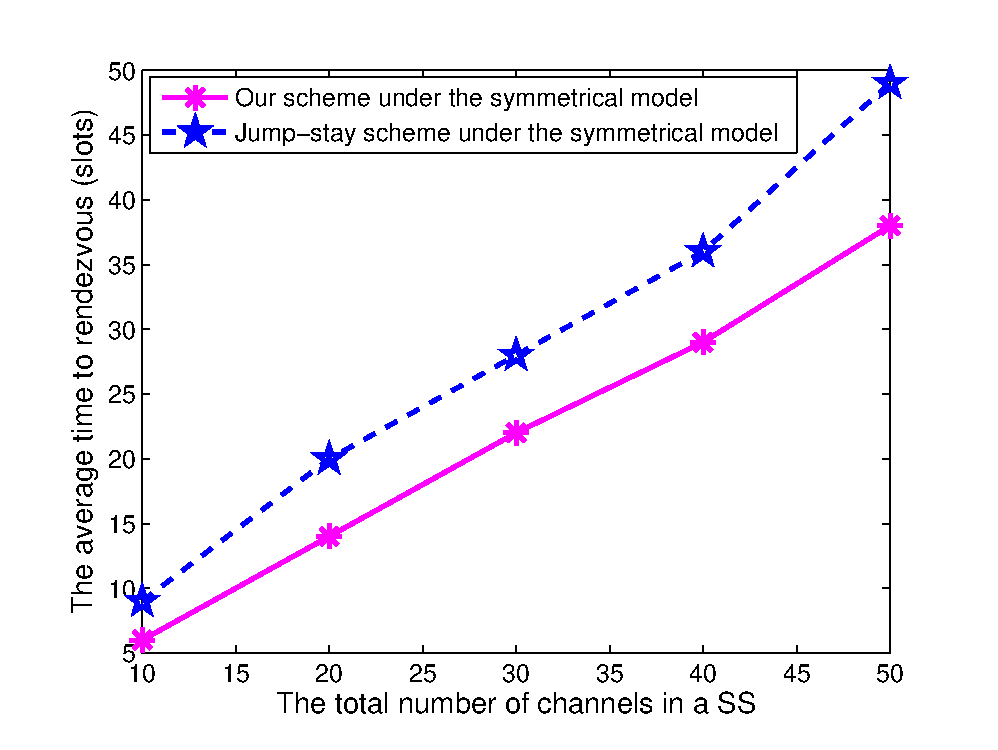
\includegraphics[width=10cm,height=8cm]{sec_3_1-rend_sym1.eps}
\caption{The \textit{ETTR} within a SS under the symmetrical model}
\label{fig:rend_sym1}
\end{center}
\end{figure}

Fig. \ref{fig:rend_sym2} shows the \textit{ETTR} of our proposed scheme and
the jump-stay scheme in a wide-band scenario with the total number of channels
changing from $50$ to $300$. In this simulation, we assume that the ratio
of the  number of available channels for the SU pair to the total number
of channels in the wide-band spectrum is $0.8$ and $\theta=20$ in the spectrum
splitting scheme. The figure shows that our proposed rendezvous algorithm
can always achieve a much lower \textit{ETTR} as compared to the jump-stay
scheme in a wide-band scenario. This is because that the channel hopping
of the jump-stay scheme includes all the channels of the whole spectrum,
while our scheme can perform rendezvous in a smaller SS because of the proposed
spectrum splitting scheme. Furthermore, due to the spectrum splitting without
changing $\theta$, the performance of our scheme does not change much even
when the total number of channels increases.

\begin{figure}[hbt]
\begin{center}
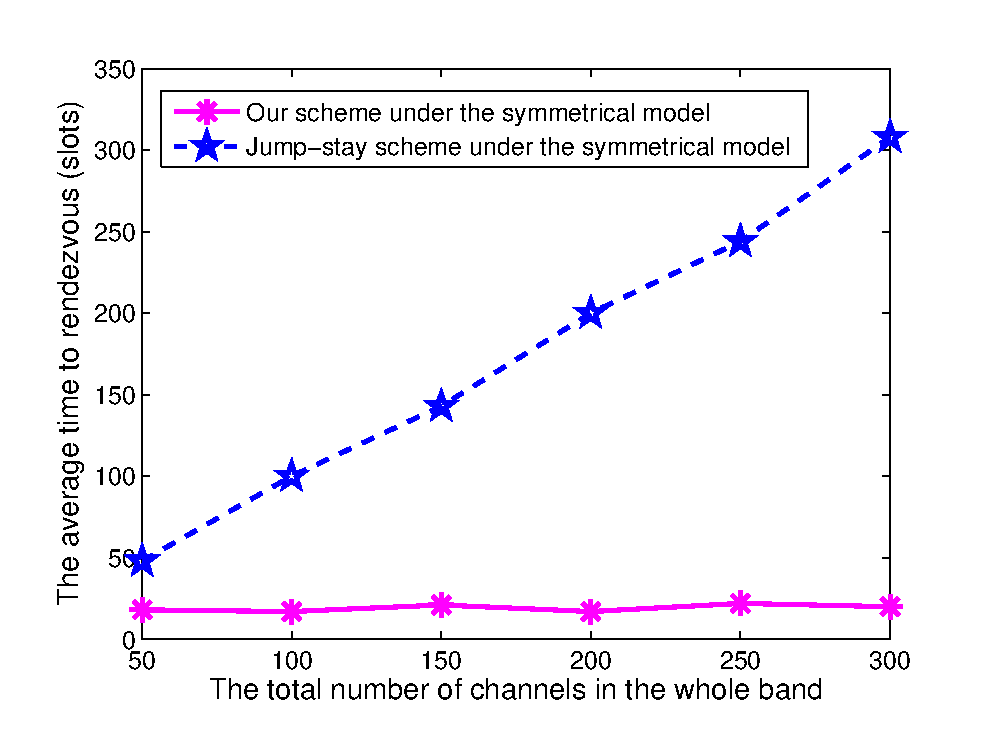
\includegraphics[width=10cm,height=8cm]{sec_3_1-rend_sym2.eps}
\caption{The \textit{ETTR} of the whole spectrum under the symmetrical model}
\label{fig:rend_sym2}
\end{center}
\end{figure}

% \begin{figure}[hbtp]
%        \centering
%        \subfigure[The \textit{ETTR} within a SS under the symmetrical model]{
%        \label{fig:rend_sym1}
%                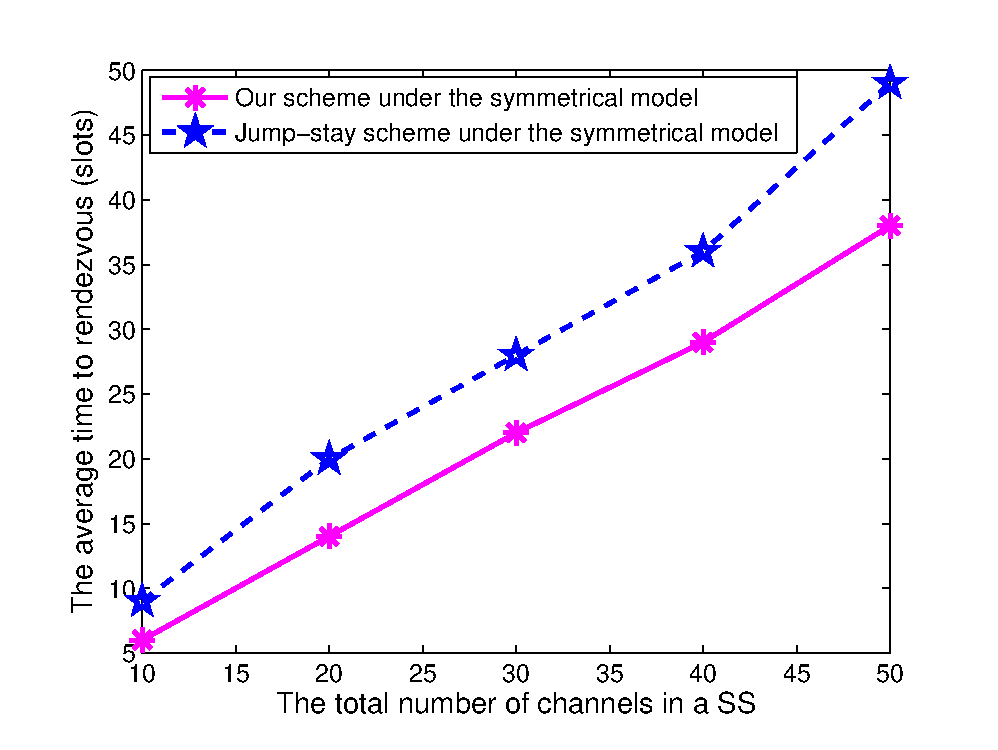
\includegraphics[width=2cm,height=5cm]{sec_3_1-rend_sym1.eps} 
%        }
%        \subfigure[The \textit{ETTR} of the whole spectrum under the symmetrical
%model]{
%        \label{fig:rend_sym2}
%        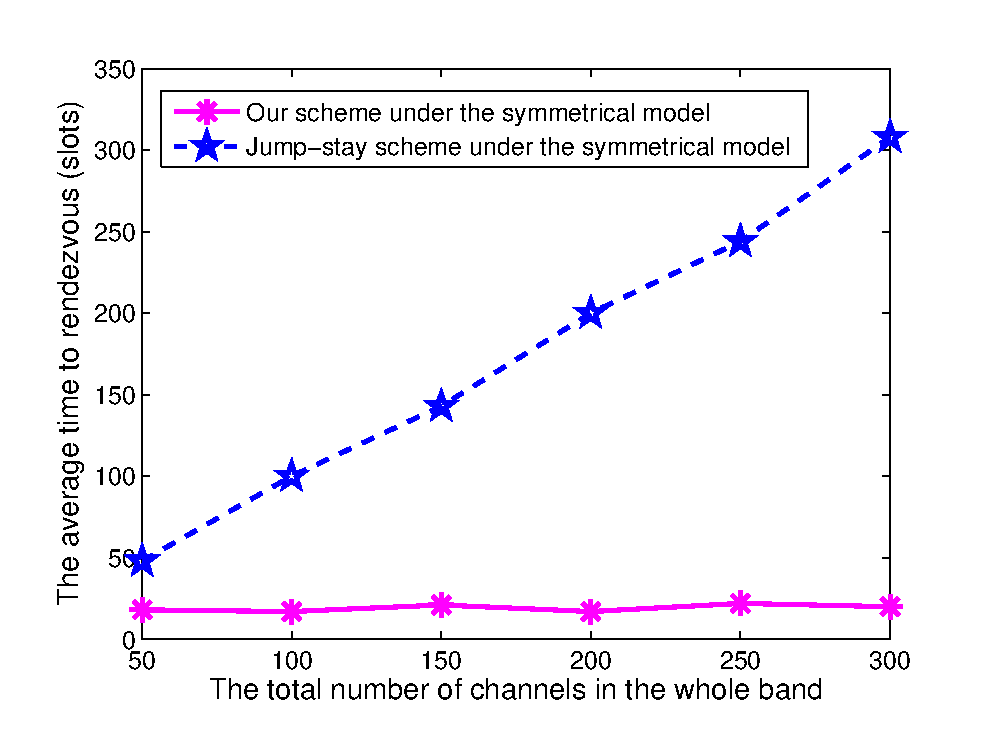
\includegraphics[width=2cm,height=5cm]{sec_3_1-rend_sym2.eps} 
%        }
%        \label{fig:rend_sym}
%        \caption{The \textit{ETTR} under the symmetrical model.}
%\end{figure}

\subsection{The \textit{ETTR}  of Rendezvous under the Asymmetrical Model}
We compare our proposed rendezvous algorithm with the jump-stay scheme \cite{zLin11JSBCH}
and enhanced jump-stay scheme \cite{zLin13EJSRA} under the asymmetrical model
which is more practical (the enhanced jump-stay scheme only considers the
asymmetrical model).

Fig. \ref{fig:rend_asym1} shows the \textit{ETTR} of our proposed scheme,
the jump-stay scheme, and the enhanced jump-stay scheme, when the SU sender
tries to rendezvous with the SU receiver whose HS has $10$ to $50$ channels.
In this simulation, we assume that the ratio of the number of available channels
for the SU pair to the total number of channels in the SU receiver's HS is
$0.5$, the SU pair has the same number of available channels, and $50\%$
of their available channels are the same.  The figure shows that the performance
of our proposed rendezvous algorithm is better than the jump-stay scheme
and enhanced jump-stay scheme under the asymmetrical model within a single
SS.

\begin{figure}[hbt]
\begin{center}
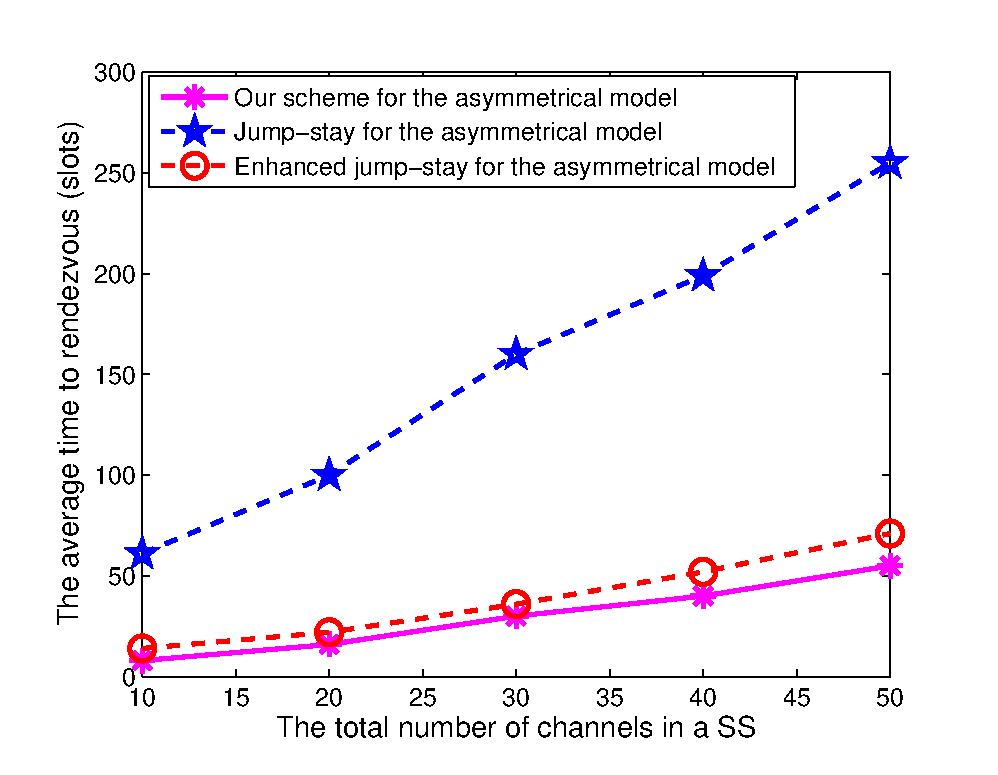
\includegraphics[width=10cm,height=8cm]{sec_3_1-rend_asym1.eps}
\caption{The \textit{ETTR} within a SS under the asymmetrical model.}
\label{fig:rend_asym1}
\end{center}
\end{figure}

Fig. \ref{fig:rend_asym2} shows the \textit{ETTR} of our proposed scheme,
the jump-stay scheme, and the enhanced jump-stay scheme in a wide-band scenario
with the total number of channels changing from $50$ to $300$. In this simulation,
we assume that $\theta=20$ in the spectrum splitting scheme, the ratio of
the number of available channels for the SU pair to the total number of channels
in the whole wide-band spectrum is $0.5$, the SU pair has the same number
of available channels, and $80\%$ of their available channels are the same.
This figure shows that the performance of our proposed rendezvous algorithm
is always much better than the jump-stay scheme and the enhanced jump-stay
scheme in a wide-band scenario. 

\begin{figure}[hbt]
\begin{center}
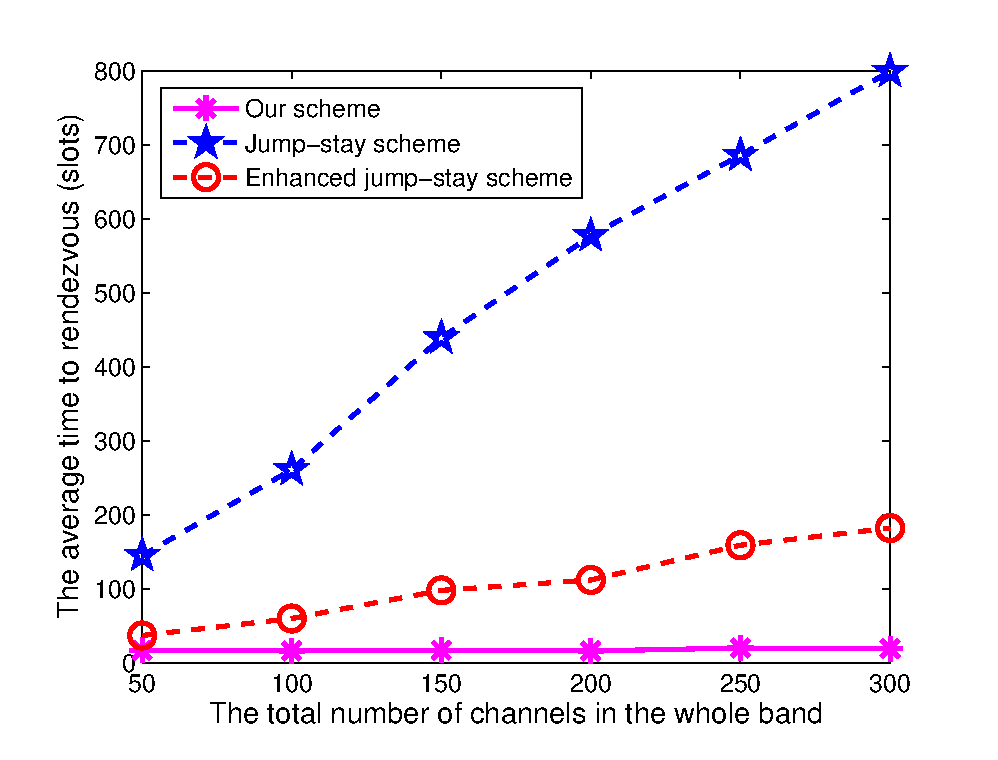
\includegraphics[width=10cm,height=8cm]{sec_3_1-rend_asym2.eps}
\caption{The \textit{ETTR} of the whole spectrum under the asymmetrical
model.}
\label{fig:rend_asym2}
\end{center}
\end{figure}

% \begin{figure}[hbtp]
%        \centering
%        \subfigure[The \textit{ETTR} within a SS under the asymmetrical model]{
%        \label{fig:rend_asym1}
%                \includegraphics[width=4cm,height=5cm]{rend_asym1.eps} 
%        }
%        \subfigure[The \textit{ETTR} of the whole spectrum under the asymmetrical
%model]{
%        \label{fig:rend_asym2}
%        \includegraphics[width=4cm,height=5cm]{rend_asym2.eps} 
%        }
%        \label{fig:rend_asym}
%        \caption{The \textit{ETTR}  under the asymmetrical model.}
%\end{figure}

 Fig. \ref{fig:com_avai_fac} shows the \textit{ETTR} of our proposed scheme,
the jump-stay scheme, and the enhanced jump-stay scheme within a SS with
a total of $40$ channels when the ratio (defined as the common available
ratio) of the number of common available channels between two SUs to the
number of their individual total available channels (assume each SU has the
same number of available channels) changes from $0.1$ to $0.9$. In this simulation,
we assume that the ratio of the number of available channels for the SU pair
to the total number of channels in the SS is $0.5$. This figure shows that
the performance of our proposed rendezvous algorithm is always much better
than the jump-stay scheme. Our scheme performs better than the enhanced jump-stay
scheme when the common available ratio changes from $0.1$ to $0.5$ and performs
almost the same as the enhanced jump-stay scheme when the common available
ratio changes from $0.6$ to $0.9$, which means that  our scheme has an advantage
when the available channel sets of the two SUs are more  distinct.
\begin{figure}[hbtp] 
    \begin{center} 
      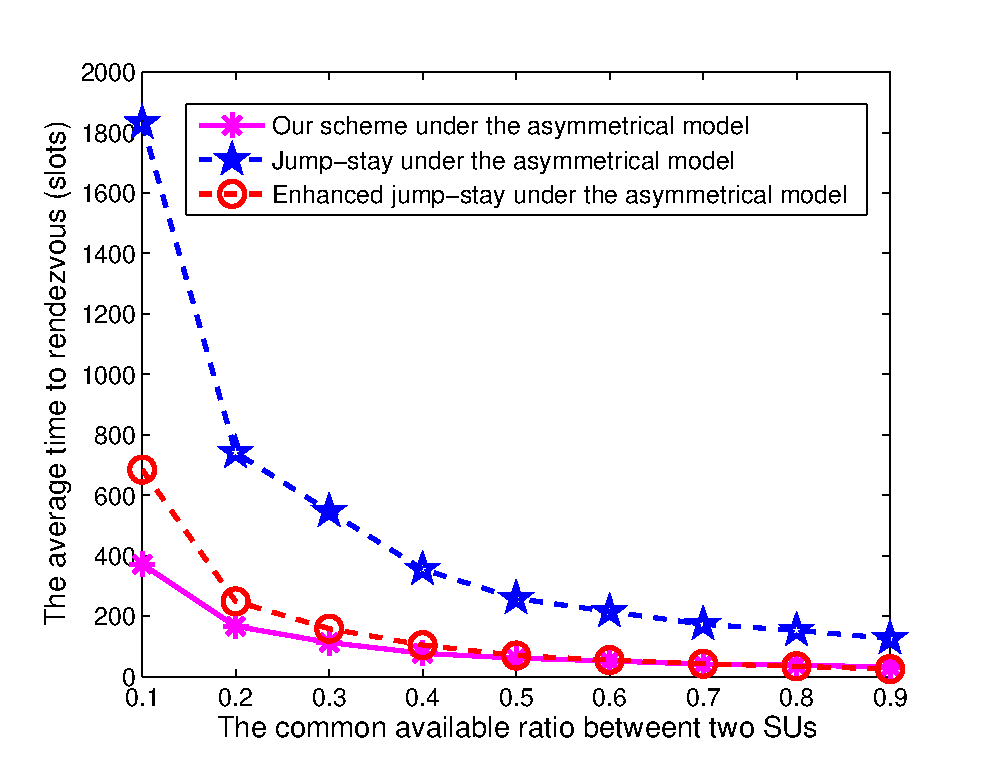
\includegraphics[width=10cm,height=8cm]{sec_3_1_com_avai_fac.eps} 
      \caption{The \textit{ETTR} under different common available ratio.}
    \label{fig:com_avai_fac} 
    \end{center}   
\end{figure} 

\subsection{The Time for Information Exchange}
As we discussed in Section \ref{sec:framework}, in order to get the control
information of other SUs, a SU has to periodically hop to each spectrum segment
(SS) to rendezvous with a SU currently in that SS and exchanges their own
and known control information. In this subsection, we show simulation results
on the time of this process. In the following simulations, the same spectrum
splitting scheme is applied for all the three rendezvous schemes and each
SU's neighbors are randomly generated to form a practical multiple-hop network.
We assume that a SU can only rendezvous with its one-hop neighbors.\\

First, we consider how long it  takes for a SU to finish hopping and rendezvousing
within all the SSs, assuming that during the process, other SUs only hop
within their home SS. This simulates the scenario that a newly joined SU
tries to get other SUs' control information. As discussed in Section  \ref{sec:framework},
a SU will hop to the next SS only after it has rendezvoused with a SU in
the current SS or it has stayed in that SS for more than MTTR time slots,
where MTTR is the maximum time to guarantee a rendezvous for the applied
rendezvous algorithm.\\

Fig. \ref{fig:oneSuSs1} shows the time for a SU to finish hopping within
all the SSs under the three rendezvous schemes, when the total number of
channels $M$ changes from $50$ to $150$ and the number of SUs $N$ is $20$.
Our proposed scheme has the same good performance as the enhanced jump-stay
scheme and outperforms the original jump-stay scheme when $M$ is below $150$,
while outperforms the other two jump-stay schemes when $M$ changes from $200$
to $300$. The reason is that our rendezvous scheme can achieve the fastest
rendezvous  and has the smallest MTTR among all the three schemes. The time
increases drastically when $M$ changes from $150$ to $300$, due to the increase
of the number of SSs and the decrease of the number of SUs in a SS.

\begin{figure}[hbtp] 
    \begin{center} 
      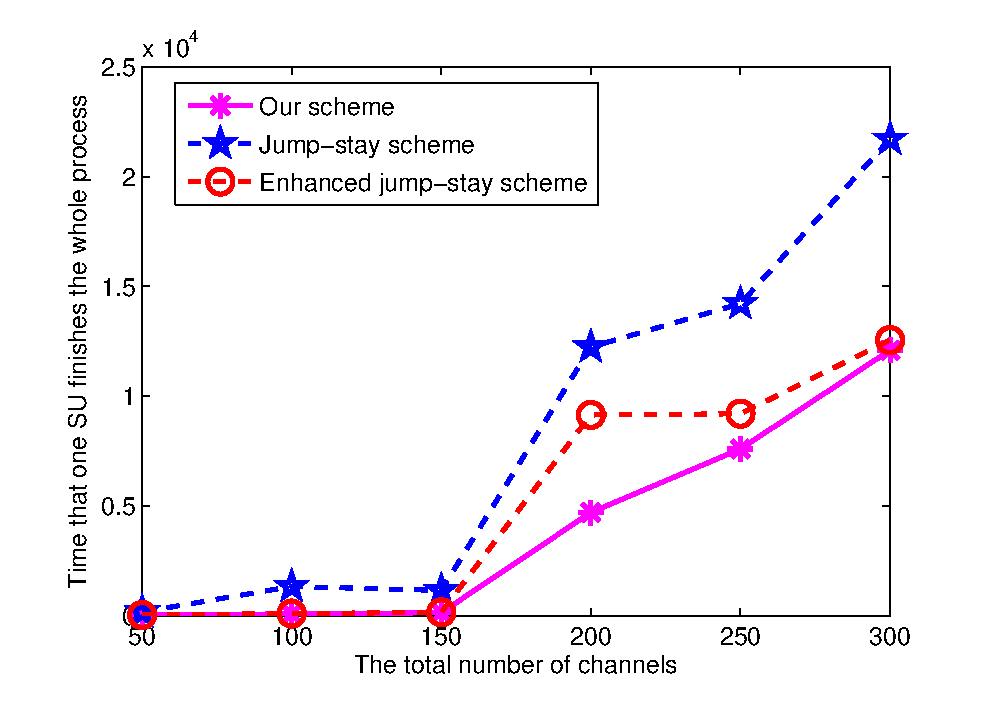
\includegraphics[width=10cm,height=8cm]{sec_3_1_oneSuSs1.eps} 
      \caption{The time for a SU to finish the whole information exchange
process as $M$ increases.}
        \label{fig:oneSuSs1} 
    \end{center}   
\end{figure} 

Fig. \ref{fig:oneSuSs2} shows the time to finish the whole information exchange
process when the number of SUs $N$ changes from $10$ to $50$ and the total
number of channels $M$ is $100$. Our proposed scheme has the same good performance
as the enhanced jump-stay scheme when $N=10,40,50$ and always outperforms
the original jump-stay scheme. However, our scheme performs much better than
the other two schemes when $N=20,30$. The vibration of the results comes
from the trade-off that when $N$ increases, the chance to achieve a rendezvous
in one SS increases, but the probability that a collision happens also increases.\\

\begin{figure}[hbtp] 
    \begin{center} 
      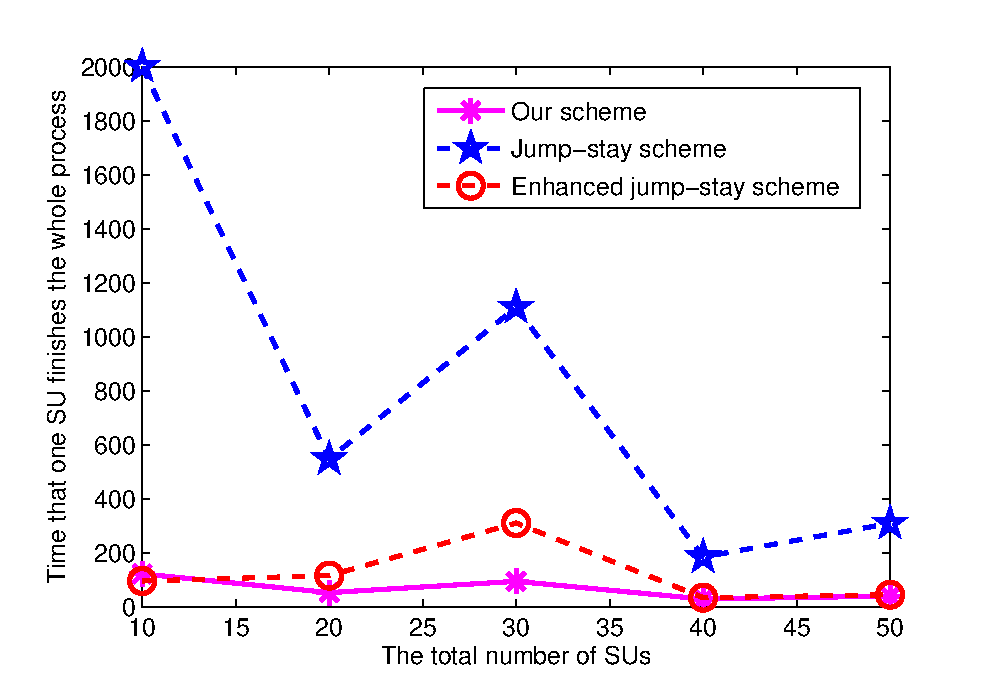
\includegraphics[width=10cm,height=8cm]{sec_3_1_oneSuSs2.eps} 
      \caption{The time for a SU to finish the whole information exchange
process as $N$ increases.}
    \label{fig:oneSuSs2} 
    \end{center}   
\end{figure} 

% \begin{figure}[hbtp]
%        \centering
%        \subfigure[Time as $M$ increases]{
%        \label{fig:oneSuSs1}
%                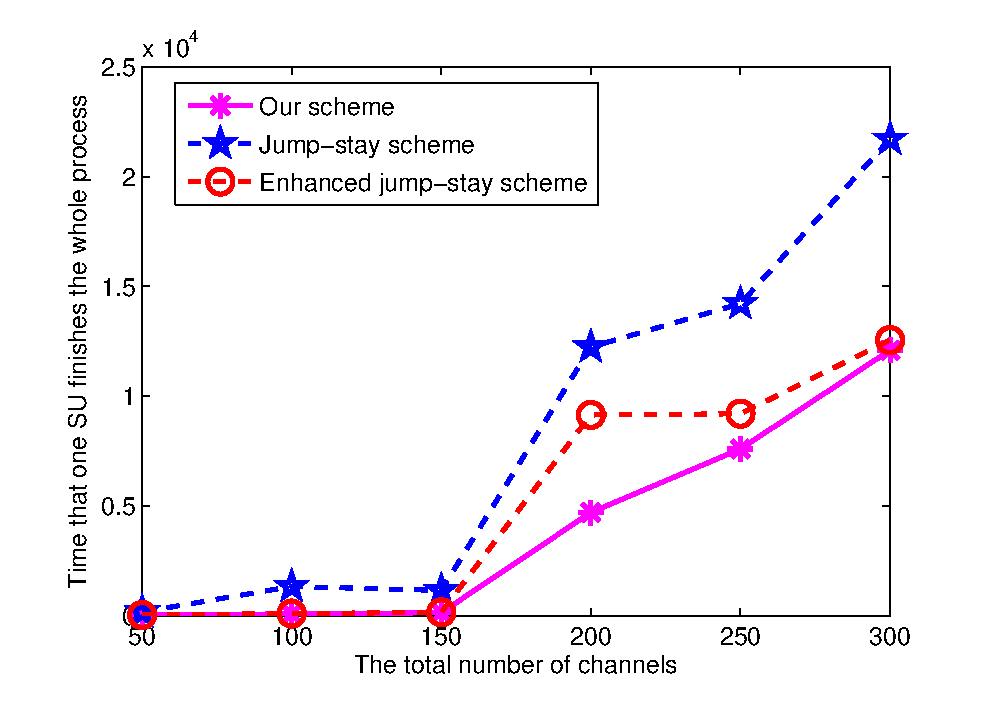
\includegraphics[width=4cm,height=5cm]{sec_3_1_oneSuSs1.eps} 
%        }
%        \subfigure[Time as $N$ increases]{
%        \label{fig:oneSuSs2}
%        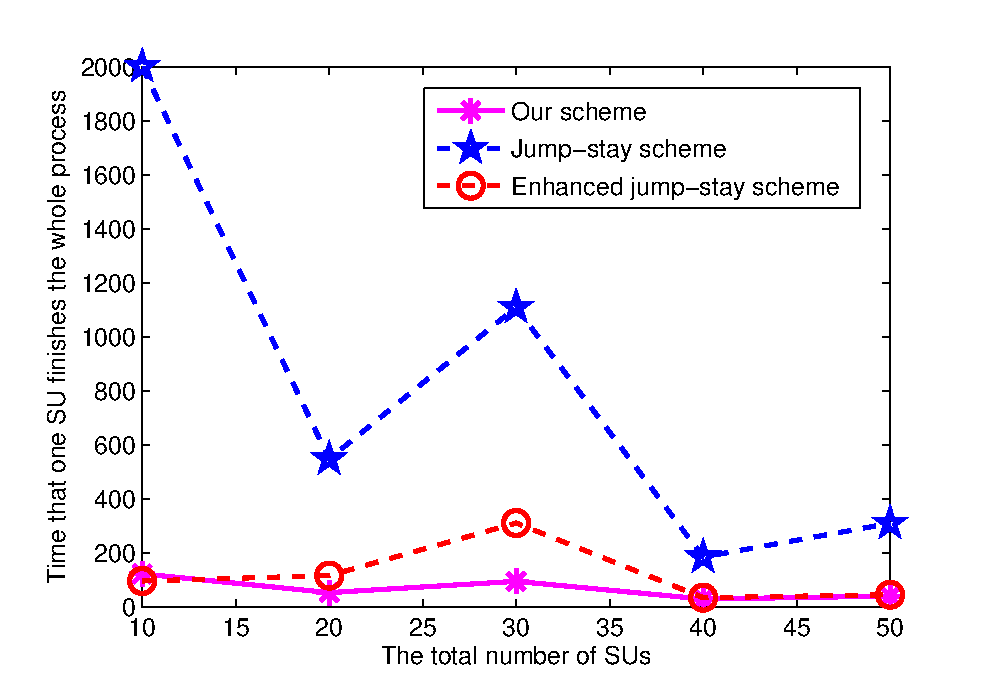
\includegraphics[width=4cm,height=5cm]{sec_3_1_oneSuSs2.eps} 
%        }
%        \label{fig:oneSuSs}
%        \caption{The time for a SU to finish the whole information exchange
%process.}
%\end{figure}

Second, we consider how long it takes all SUs to finish hopping and rendezvousing
within all the SSs, assuming that all the SUs start this process simultaneously.
This simulates the scenario that several SUs start to form a CRN and try
to get other SUs' control information. 

Fig. \ref{fig:allSuSs1} shows the
time for all SUs to finish the whole process , when $N=20$ and $M$ changes
from $50$ to $300$. In this figure, our proposed scheme outperforms both
jump-stay schemes because of faster rendezvous and smaller MTTR. The time
increases with $M$ since more channels increase the time to rendezvous.

\begin{figure}[hbtp] 
    \begin{center} 
      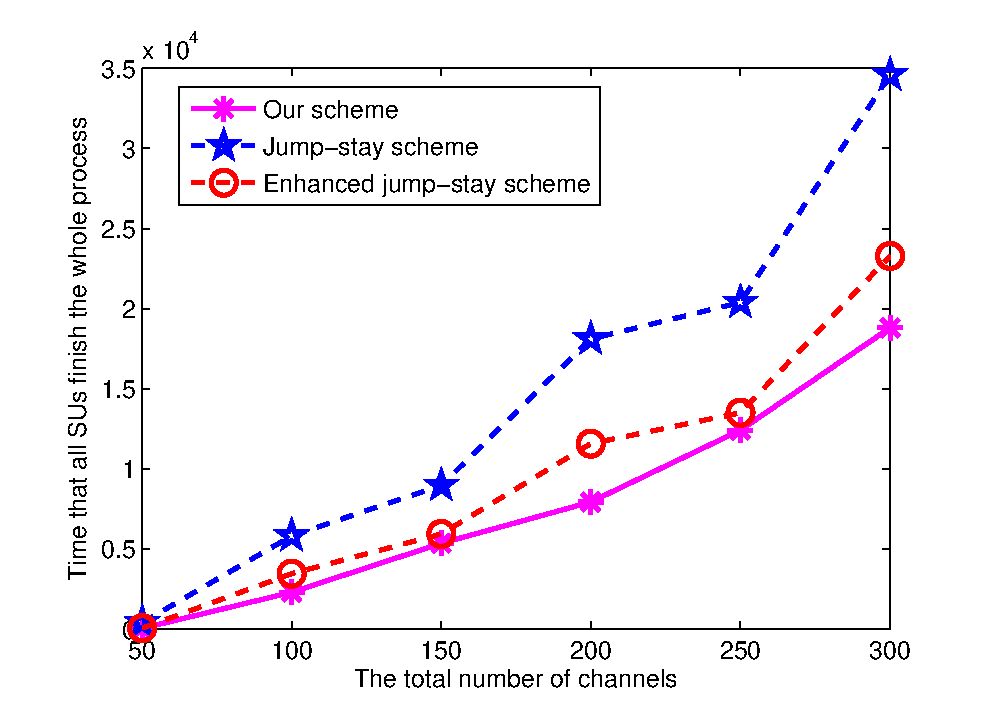
\includegraphics[width=10cm,height=8cm]{sec_3_1_allSuSs1.eps} 
      \caption{The time for all SUs to finish the whole information exchange
process as $M$ increases.}
    \label{fig:allSuSs1} 
    \end{center}   
\end{figure} 

Fig. \ref{fig:allSuSs2} shows the time for all SUs to finish the whole process,
when $M=100$ and $N$ changes from $10$ to $50$. Our scheme still outperforms
the other two jump-stay schemes. The time to finish the whole process decreases
as $N$ increases. This is because that more SUs in the whole network results
in more SUs in a SS, which increases the chance of one SU to rendezvous with
each other.

\begin{figure}[hbtp] 
    \begin{center} 
      \includegraphics[width=10cm,height=8cm]{sec_3_1_allSuSs2.eps} 
      \caption{The time for all SUs to finish the whole information exchange
process as $N$ increases.}
    \label{fig:allSuSs2} 
    \end{center}   
\end{figure} 

% \begin{figure}[hbtp]
%        \centering
%        \subfigure[Time as $M$ increases]{
%        \label{fig:allSuSs1}
%                \includegraphics[width=4cm,height=5cm]{allSuSs1.eps} 
%        }
%        \subfigure[Time as $N$ increases]{
%        \label{fig:allSuSs2}
%        \includegraphics[width=4cm,height=5cm]{allSuSs2.eps} 
%        }
%        \label{fig:allSuSs}
%        \caption{The time for all SUs to finish the whole information exchange
%process.}
%\end{figure}

Therefore, our proposed scheme outperforms the two jump-stay schemes when
considering a practical CRN where the control information exchange and update between SUs are necessary.

\subsection{The Average Normalized Throughput}
We consider practical communication scenarios in a CRN with multiple SU pairs
and traffic flows. We evaluate  the average normalized throughput for each
user in a CRN which is the average ratio of the number of data packets successfully
transmitted out by a SU sender to the total number of data packets generated
in a period of time. Since there are no other existing similar rendezvous
schemes deigned for wide-band CRNs considering the practical communication
scenario we consider here, we apply both jump-stay and enhanced jump-stay
rendezvous schemes to a wide-band CRN under both the symmetrical and asymmetrical models. We assume that there are $30$ SUs in the network: $15$ are the SU
senders and $15$ are the SU receivers. The average packet arrival rate for
each SU sender is $5\ packets/sec$. The length of each packet in the unit
of time slots is a random number in $[1,20]$. We assume that $\theta=20$,
the total number of channels in the wide-band CRN changes from $50$ to $300$,
and the ratio of the number of available channels for the SU pair to the
total number of channels in the whole wide-band spectrum is $0.8$.\\

 Fig. \ref{fig:thru_sym1} shows the average normalized throughput of our
proposed scheme   and the jump-stay scheme under the symmetrical model when
the total number of channels within a wide-band spectrum changes from $50$
to $300$. The result shows that our proposed scheme can maintain a very high
average normalized throughput which is much better than the jump-stay scheme
when considering the whole wide-band spectrum. This is because that after
splitting the spectrum, the time to rendezvous of each transmission pair
is much shorter. Thus, the overall throughput is benefited.

\begin{figure}[hbtp] 
    \begin{center} 
      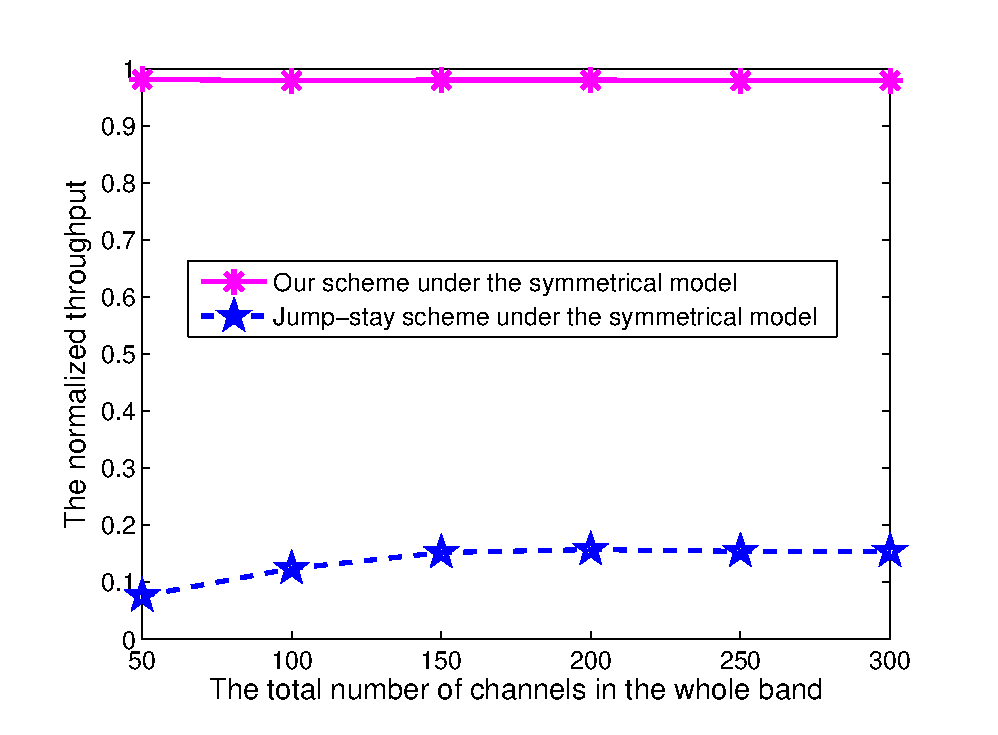
\includegraphics[width=10cm,height=8cm]{sec_3_1_thru_sym1.eps} 
      \caption{The average normalized throughput under the symmetrical
model as the number of total channels increases.}
    \label{fig:thru_sym1} 
    \end{center}   
\end{figure} 
 
Fig. \ref{fig:thru_sym2} shows the average normalized throughput of our proposed
scheme and the jump-stay scheme under the symmetrical model when the SU packet
arrival rate changes from $1$ to $20$. We consider a wide-band spectrum with
$200$ channels here. The result shows that our proposed scheme can maintain
a very high average normalized throughput which is much better than the jump-stay
scheme under different SU packet arrival rates. We can also notice that the
average normalized throughput of the jump-stay scheme decreases significantly
when the SU packet arrival rate increases, while our scheme can still keep
a high throughput. 

\begin{figure}[hbtp] 
    \begin{center} 
      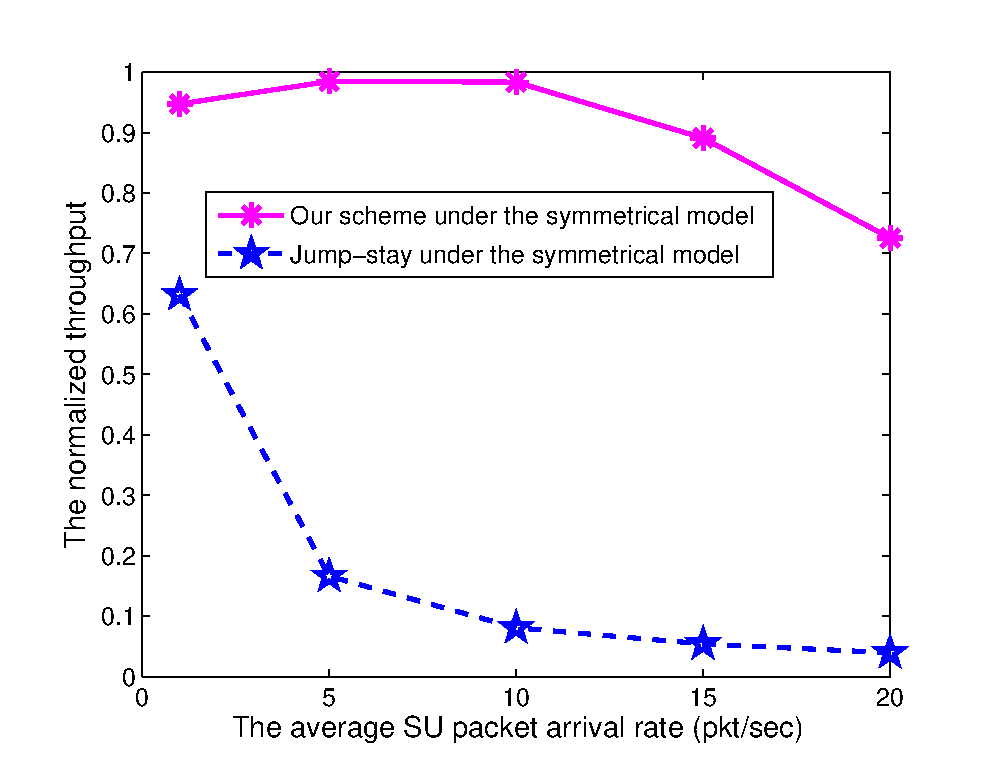
\includegraphics[width=10cm,height=8cm]{sec_3_1_thru_sym2.eps} 
      \caption{The average normalized throughput under the symmetrical
model as the SU packet arrival rate increases.}
    \label{fig:thru_sym2} 
    \end{center}   
\end{figure} 

% \begin{figure}[hbtp]
%        \centering
%        \subfigure[The effect of the number of total channels]{
%        \label{fig:thru_sym1}
%                \includegraphics[width=4cm,height=5cm]{thru_sym.eps} 
%        }
%        \subfigure[The effect of SU packet arrival rate]{
%        \label{fig:thru_sym2}
%        \includegraphics[width=4cm,height=5cm]{thru_sym2.eps} 
%        }
%        \label{fig:thru_sym}
%        \caption{The average normalized throughput under the symmetrical
%model.}
%\end{figure}

Fig. \ref{fig:thru_asym1} shows the average normalized throughput of our
proposed scheme, the jump-stay scheme, and the enhanced jump-stay scheme
under the asymmetrical model when the total number of channels varies from
$50$ to $300$. The result shows that the average normalized throughput of
our proposed scheme is much higher than that of the jump-stay scheme and
enhanced jump-stay scheme when the whole wide-band spectrum is considered.
We can also notice that the performance of the jump-stay scheme and the enhanced
jump-stay scheme fluctuates with the increment of the total number of  channels,
while our scheme can still keep a high normalized throughput because of the
proposed  framework and rendezvous schemes.

\begin{figure}[hbtp] 
    \begin{center} 
      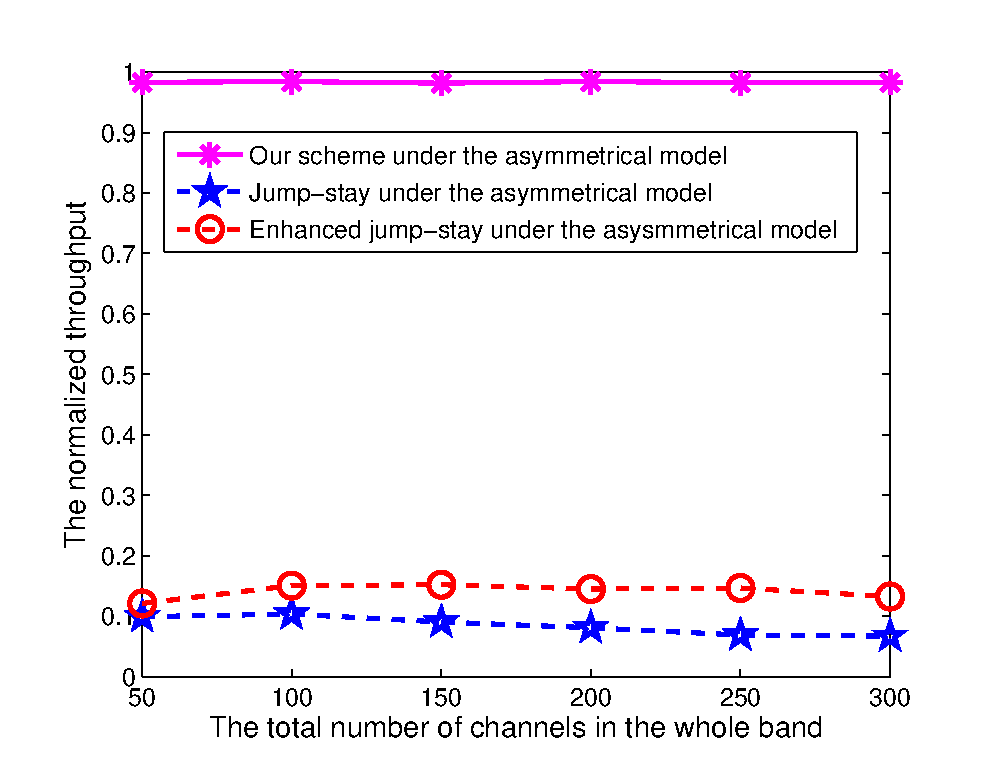
\includegraphics[width=10cm,height=8cm]{sec_3_1_thru_asym1.eps} 
      \caption{The average normalized throughput under the asymmetrical
model as  the number of total channels increases.}
    \label{fig:thru_asym1} 
    \end{center}   
\end{figure} 

 Fig. \ref{fig:thru_asym2} shows the average normalized throughput of our
proposed scheme, the jump-stay scheme, and the enhanced jump-stay scheme
under the asymmetrical model when the SU packet arrival rate changes from
$1$ to $20$. We consider a wide-band spectrum with $200$ channels. The result
shows that our proposed scheme performs much better than both the jump-stay
scheme and enhanced jump-stay scheme when the SU packet arrival rate changes.
Therefore, our proposed scheme can adapt to different SU traffic under the
asymmetrical model.

\begin{figure}[hbtp] 
    \begin{center} 
      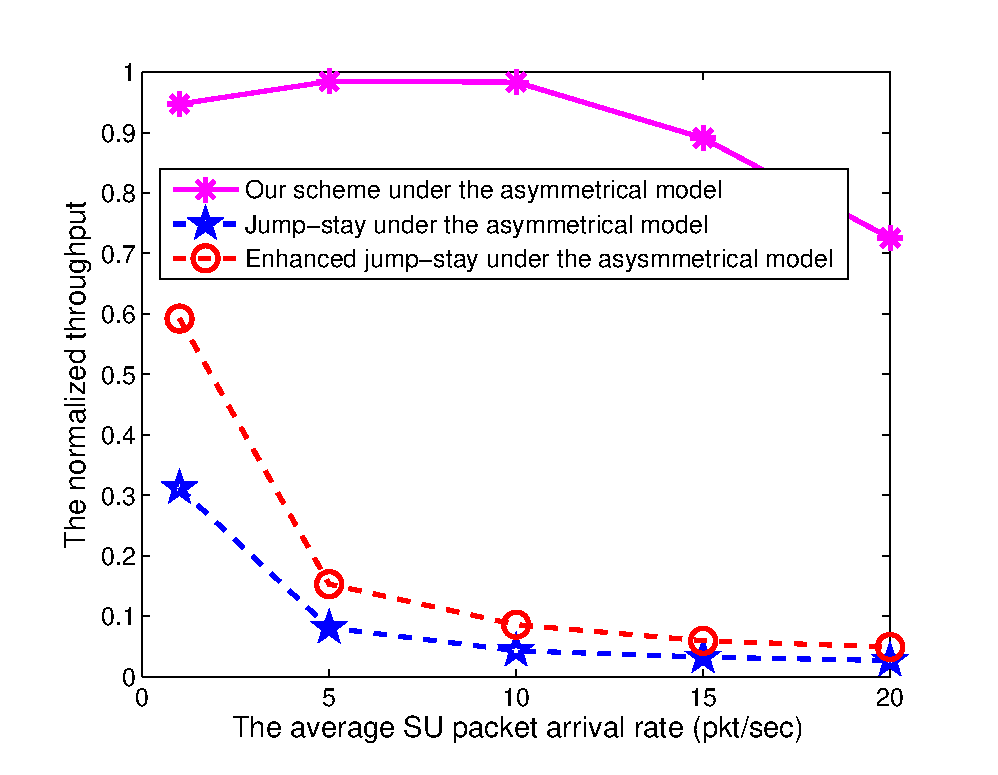
\includegraphics[width=10cm,height=8cm]{sec_3_1_thru_asym2.eps} 
      \caption{The average normalized throughput under the asymmetrical
model as the SU packet arrival rate increases.}
    \label{fig:thru_asym2} 
    \end{center}   
\end{figure} 

%\begin{figure}[hbtp]
%        \centering
%        \subfigure[The results of the number of total channels]{
%        \label{fig:thru_asym1}
%                \includegraphics[width=4cm,height=5cm]{thru_asym.eps} 
%        }
%        \subfigure[The effect of SU packet arrival rate]{
%        \label{fig:thru_asym2}
%        \includegraphics[width=4cm,height=5cm]{thru_asym2.eps} 
%        }
%        \label{fig:thru_asym}
%        \caption{The average normalized throughput under the asymmetrical
%model.}
%\end{figure}

\subsection{The Effect of the Value of $\theta$}
Our spectrum splitting scheme is based on a predetermined value $\theta$.
Therefore, how to determine an  appropriate $\theta$ is crucial for our proposed
communication framework. In this subsection, we show the effect of $\theta$
on the average normalized throughput and the average collision ratio which
can help us to determine $\theta$ under both the symmetrical and asymmetrical
models. The average collision ratio is defined as the ratio of the number
of  successful rendezvous with collisions to the total number of rendezvous.
The parameters in the following simulation are the same as the ones in the
last subsection, except the total number of channels and $\theta$. We set
the total number of channels to be $100$ and change the value of $\theta$
from $10$ to $50$.\\

Fig. \ref{fig:theta_sym1} shows the effect of $\theta$ under the symmetrical
model on the average normalized throughput. When $\theta$ increases, the
number of channels in each SS increases. This may result in a longer time
to rendezvous in our proposed scheme. Thus, the average normalized throughput
decreases. 

\begin{figure}[hbtp] 
    \begin{center} 
      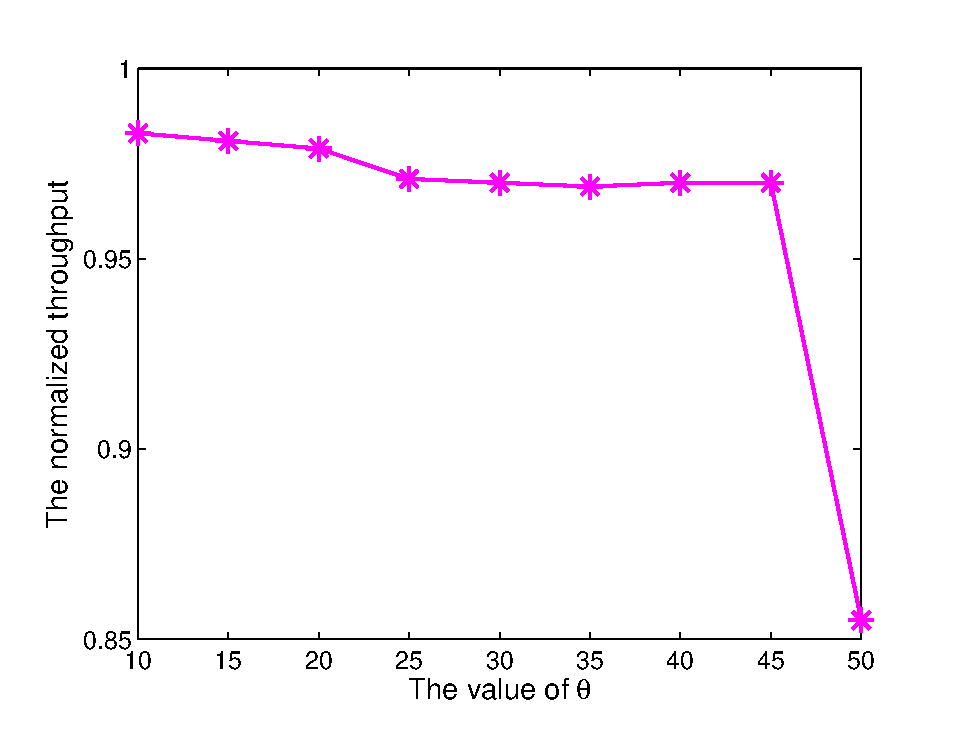
\includegraphics[width=10cm,height=8cm]{sec_3_1_theta_sym1.eps} 
      \caption{The effect of $\theta$ to the throughput under the symmetrical model.}
    \label{fig:theta_sym1} 
    \end{center}   
\end{figure} 

Fig. \ref{fig:theta_sym2} shows the effect of $\theta$ on the
average collision ratio under the symmetrical model. When $\theta$ increases,
the average collision ratio decreases. This is reasonable since when $\theta$
increases, a SU pair can rendezvous on more channels in a SS. Thus, the probability
that multiple SUs rendezvous on the same channel is reduced. By observing
Fig. \ref{fig:theta_sym1} and Fig. \ref{fig:theta_sym2} together, we can
notice that when the collision ratio increases, the average normalized throughput
increases also. This indicates that the rendezvous collisions under the symmetrical
model may not affect the throughput.

\begin{figure}[hbtp] 
    \begin{center} 
      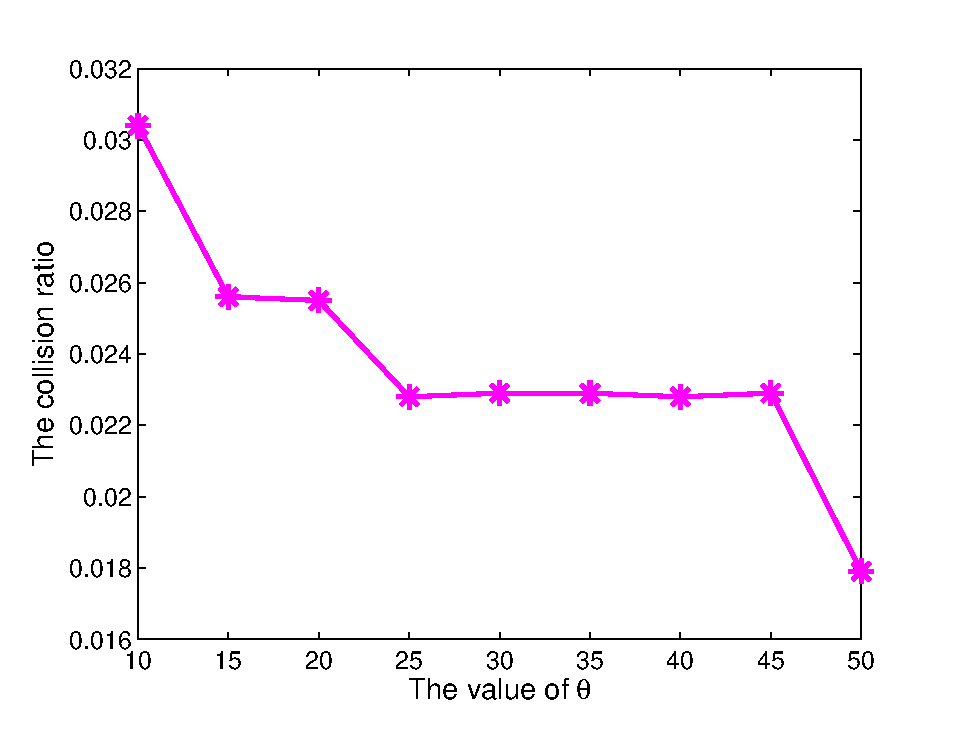
\includegraphics[width=10cm,height=8cm]{sec_3_1_theta_sym2.eps} 
      \caption{The effect of $\theta$ to the collision ratio under the symmetrical model.}
    \label{fig:theta_sym2} 
    \end{center}   
\end{figure} 

%\begin{figure}[hbtp]
%        \centering
%        \subfigure[The effect of $\theta$ to the throughput]{
%        \label{fig:theta_sym1}
%                \includegraphics[width=4cm,height=5cm]{theta_sym1.eps} 
%        }
%        \subfigure[The effect of $\theta$ to the collision ratio]{
%        \label{fig:theta_sym2}
%        \includegraphics[width=4cm,height=5cm]{theta_sym2.eps} 
%        }
%        \label{fig:theta_sym}
%        \caption{The effect of $\theta$ under the symmetrical model.}
%\end{figure}

Fig. \ref{fig:theta_asym1} shows the effect of $\theta$ under the asymmetrical
model on the average normalized throughput. When $\theta$ increases, the
average normalized throughput  first increases and then decreases. The reason
is that under the asymmetrical model, each SU will use all the channels in
a SS to design a channel hopping sequence. When the number of channels in
a SS is small, the \textit{ETTR} decreases, but the probability of a collision
between  the communicating pairs in the same SS increases, which may decease
the average normalized throughput. On the other hand, when the number of
channels in a SS increases, the \textit{ETTR}  increases, which can also
decrease the average normalized throughput. Therefore, there exists an optimal
$\theta$ for the asymmetrical model to maximize the average normalized throughput.
Under this particular scenario, we can set $\theta$ to be $35$ or $40$ to
get the maximum average normalized throughput. 

\begin{figure}[hbtp] 
    \begin{center} 
      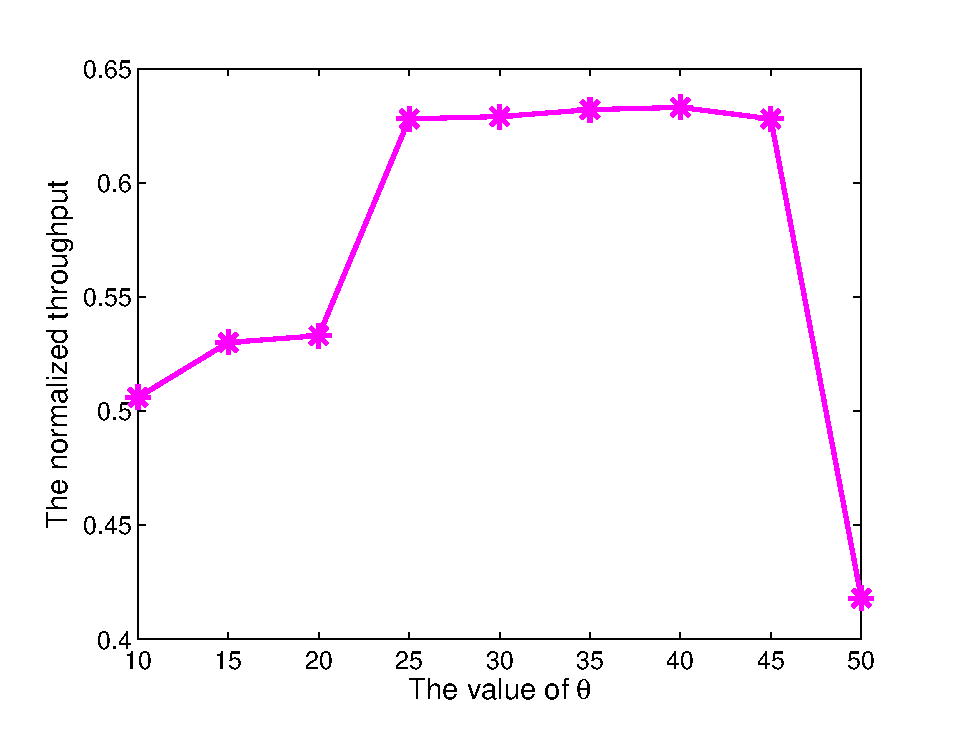
\includegraphics[width=10cm,height=8cm]{sec_3_1_theta_asym1.eps} 
      \caption{The effect of $\theta$ to the throughput under the asymmetrical model.}
    \label{fig:theta_asym1} 
    \end{center}   
\end{figure} 


Fig. \ref{fig:theta_asym2}
shows the effect of $\theta$ on the average collision ratio under the asymmetrical
model. When $\theta$ increases, the collision ratio decreases. By observing
Fig. \ref{fig:theta_asym1} and Fig. \ref{fig:theta_asym2} together, we can
notice that when the collision ratio decreases, the throughput fluctuates.
This indicates that the rendezvous collision under the asymmetrical model
is a factor which can affect the throughput.

\begin{figure}[hbtp] 
    \begin{center} 
      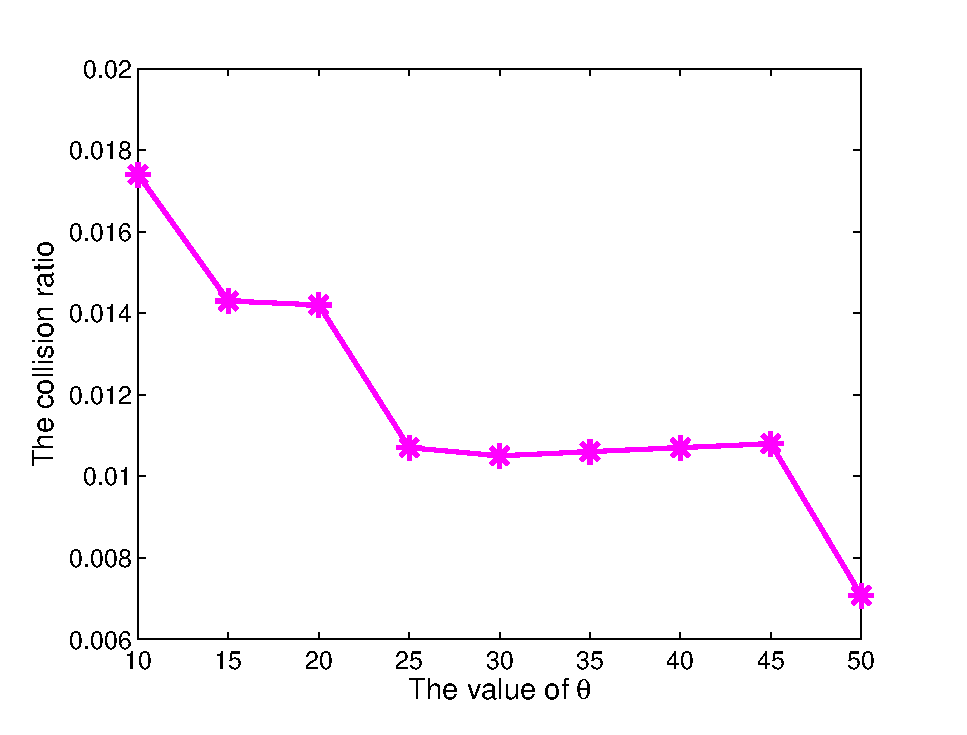
\includegraphics[width=10cm,height=8cm]{sec_3_1_theta_asym2.eps} 
      \caption{The effect of $\theta$ to the collision ratio under the asymmetrical model.}
    \label{fig:theta_asym2} 
    \end{center}   
\end{figure} 

%\begin{figure}[hbtp]
%        \centering
%        \subfigure[The effect of $\theta$ to the throughput]{
%        \label{fig:theta_asym1}
%                \includegraphics[width=4cm,height=5cm]{theta_asym1.eps} 
%        }
%        \subfigure[The effect of $\theta$ to the collision ratio]{
%        \label{fig:theta_asym2}
%        \includegraphics[width=4cm,height=5cm]{theta_asym2.eps} 
%        }
%        \label{fig:theta_asym}
%        \caption{The effect of $\theta$ under the asymmetrical model.}
%\end{figure}

Based on the above analysis, when the system performance requirements are
given, an appropriate $\theta$ can be predetermined. 

\chapter{Rendezvous Schemes Without Predetermined Sender and Receiver Considering  Multiple Cognitive Radios}
\label{chapter_mul_radios}
In this section, we propose two efficient rendezvous schemes under the scenarios that
there is not a predetermined sender or receiver for a rendezvous process
during the initialization phase of cognitive radio networks when SUs are equipped with multiple radios.
\section{System Model and Problem Description}
\label{sec_3_2_pro}
In this research, we assume that there are totally $N$ SUs and $N_{p}$ PUs coexisting. There are totally $M$ channels that all the SUs and PUs can access.  Each SU is equipped with a GPS  which can get its location coordinates. Furthermore, each SU is equipped with exactly $R$  homogeneous
half-duplex cognitive radios. Therefore, a cognitive radio cannot send and receive signals simultaneously. We assume that for a SU, all its cognitive radios use the same transmission power and have the same interference range.

There is no CCC in the network through which all SUs can exchange their control information. Before the initialization process of a CRN, each SU does not know any information about other SUs, which is a very practical assumption. A time-slotted system is deployed among all SUs and they do no need to be strictly synchronized.

A channel hopping scheme is adopted for the rendezvous process. During a rendezvous process, each cognitive radio of an SU hops to a  channel chosen from its available channel set, senses the current availability of the channel, and sends an RTS packet or waits for an RTS packet from another SU. Therefore, each time slot includes the sensing phase and the sending or receiving phase during the rendezvous process. According to existing rendezvous schemes, a successful rendezvous occurs when  two SUs hop to a common available channel at the same time slot, but the process of sending an RTS packet and receiving a CTS reply is not considered. In this research, we define this kind of rendezvous as  \textit{channel rendezvous}. This may not be a problem when one SU is always the sender while the other is the receiver, which means that there is an explicit send-or-receive relationship between the two SUs. Under this scenario, after one SU sends an RTS packet,  if the other SU receives the RTS packet and replies a CTS packet, the rendezvous succeeds.

However, during the initialization phase of a CRN, each SU may want to rendezvous with other SUs to exchange control information. There is no explicit role for a SU, since it cannot know if other SUs are senders or receivers currently. If two SUs hop to a common available channel and they both have their transceivers on, none of them can receive the RTS packets, which can fail a successful rendezvous. Furthermore, each SU does not know if its target SU is on the current common available channel and is sending or receiving  in the current time slot. Practically, only when the two SUs hop to a common available channel and when one SU is sending  while the other is trying to receive on that channel, a successful rendezvous can finally happen. In this research, we denote this kind of rendezvous as  \textit{link rendezvous}. Therefore, when an SU is equipped with multiple cognitive radios, during a rendezvous process, the SU should not only consider which available channel each cognitive radio should tune to but also determine that each radio should be in the sending or receiving mode. We call this problem as the \textit{send-or-receive problem} in a rendezvous scheme.

For the $i$th SU with $R$ cognitive radios, during time slot $t$ of a rendezvous process, it generates a \textit{task allocation list} $\mathbb{A}^{t}_{i} = {(c^{t}_{i1}, s^{t}_{i1}), (c^{t}_{i2}, s^{t}_{i2}), \dots, (c^{t}_{iR}, s^{t}_{iR})}$, where $1\leq c^{t}_{iu} \leq M$, $s^{t}_{iu} = 1$ (send) or $s^{t}_{iu} = 0$ (receive), and $(c^{t}_{iu}, s^{t}_{iu})$ is called a \textit{task pair} for the $u$th cognitive radio of the $i$th SU during time slot $t$. We also denote $C_{i}^{t}$ as the available channel set of the $i$th SU during  time slot $t$. We define  \textit{link rendezvous} as follows.

\textit{Link Rendezvous}: A successful link rendezvous between the $i$th SU and the $j$th SU during time slot $t$ requires that there exists a task pair $(c^{t}_{iu}, s^{t}_{iu})$ for the $u$th cognitive radio of the $i$th SU and a task pair $(c^{t}_{jv}, s^{t}_{jv})$ for the $v$th cognitive radio of the $j$th SU such that $c^{t}_{iu} \in C^{t}_{i}$, $c^{t}_{jv} \in C^{t}_{j}, c^{t}_{iu} = c^{t}_{jv}$, and $s^{t}_{iu}\ \mbox{XOR}\ s^{t}_{jv} = 1$.

Moreover,  we can notice that $\mathbb{A}^{t}_{i}$ should satisfy the following constraints:
\begin{enumerate}
\item No two task pairs $(c^{t}_{iu}, s^{t}_{iu})$ and $(c^{t}_{iv}, s^{t}_{iv})$ satisfy that $c^{t}_{iu} = c^{t}_{iv}$ and $s^{t}_{iu} = s^{t}_{iv} = 1$, which means that two cognitive radios of the same SU cannot send RTS packets simultaneously on the same channel.
\item No two task pairs $(c^{t}_{iu}, s^{t}_{iu})$ and $(c^{t}_{iv}, s^{t}_{iv})$ satisfy that $c^{t}_{iu} = c^{t}_{iv}$ and $s^{t}_{iu}\ \mbox{XOR}\ s^{t}_{iv} = 1$, which means that when one cognitive radio of an SU is sending an RTS packet, there should be no  other cognitive radio of the same SU that is trying to receive RTS packets on the same channel.
\end{enumerate}

Therefore, the problem is how to generate a \textit{task allocation list} $\mathbb{A}$ for each SU to realize a fast and guaranteed rendezvous considering the \textit{send-or-receive problem}.

\section{The Basic Rendezvous Scheme}
In this section, we discuss the blind rendezvous problem between two SUs when considering multiple cognitive radios and the \textit{send-or-receive problem}. At the beginning of the initialization phase of a CRN, each SU does not know any information about other SUs. Therefore, each SU can only perform a blind rendezvous process based on its local information to set up links with other SUs. However, previous research works only focus on designing the channel-hopping sequence so that the two SUs can hop to a common available channel at the same time, while ignore the \textit{send-or-receive problem}, especially when each SU is equipped with multiple cognitive radios. Our goal is to generate a \textit{task allocation list} for each SU during each time slot based on an existing channel hopping sequence so that two SUs can achieve a successful \textit{link  rendezvous} within bounded time slots.

Our proposed basic link rendezvous scheme is to generate a \textit{task allocation list} $\mathbb{A}$ for each SU during each time slot based on an existing channel hopping sequence which can guarantee a successful \textit{channel rendezvous} within bounded time slots. Given a specific channel hopping sequence ( e.g., the jump-stay channel hopping sequence in \cite{zLin11JSBCH}), we denote the channel-hopping sequence for the $j$th radio of the $i$th SU as $\mathbb{S}_{ij}$, and the element in $\mathbb{S}_{ij}$ at time slot $t$ as $\mathbb{S}^{t}_{ij}$. After $\mathbb{S}_{ij}$ is  generated,  for the task allocation list $\mathbb{A}^{t}_{i}$, all the values of $c^{t}_{i1}, c^{t}_{i2}, \dots, c^{t}_{iR}$ are determined as $c^{t}_{i1} = \mathbb{S}^{t}_{i1}, c^{t}_{i2} = \mathbb{S}^{t}_{i2}, \dots, c^{t}_{iR} = \mathbb{S}^{t}_{iR}$. Therefore, the next step is to set the binary values of $0$ or $1$ to $s^{t}_{i1}, s^{t}_{i2}, \dots, s^{t}_{iR}$ to guarantee that $\mathbb{A}^{t}_{i}$ satisfy the constraints explained in Section \ref{sec_3_2_pro}.

For any $c^{t}_{ij}, 1\leq j \leq R$, if $c^{t}_{ij}$ appears more than once among all the $R$ radios, which means that more than one radio will hop on channel $c^{t}_{ij}$ during time slot $t$, the radios allocated to channel $c^{t}_{ij}$ should wait for RTS packets according to the constraints in Section \ref{sec_3_2_pro}   Other radios will randomly choose sending or receiving roles to themselves.

Here is an example of the $0-1$ allocation solution. Assume that $R = 5$ and $c^{t}_{i1} = 1, c^{t}_{i2} = 3, c^{t}_{i3} = 3, c^{t}_{i4} = 2, c^{t}_{i5} = 1$. Since channel $3$ appears twice, $s^{t}_{i2} = 0$ and $s^{t}_{i3} = 0$, which means that the second and third radio should wait for RTS packets during the current time slot on channel $3$. Since channel $1$  also appears twice, $s^{t}_{i1} = 0$ and $s^{t}_{i5} = 0$, which means that the first and fifth radio should also wait for RTS packets during the current time slot on channel $1$. For the fourth radio, we can randomly set $s^{t}_{i4} = 1$.  Finally, the generated \textit{task allocation list} for the $i$th SU during time slot $t$ is $\mathbb{A}^{t}_{i} = \{(c^{t}_{i1} = 1, s^{t}_{i1} = 0), (c^{t}_{i2} = 3, s^{t}_{i2} = 0), (c^{t}_{i3} = 3, s^{t}_{i3} = 0), (c^{t}_{i4} = 2, s^{t}_{i4} = 1), (c^{t}_{i5} = 1, s^{t}_{i5} = 0)\}$.

The details of our proposed rendezvous scheme for the $i$th SU is shown in \textbf{Algorithm \ref{al:basic}}.

\begin{algorithm} 
  \caption{The basic rendezvous algorithm considering the send-or-receive problem}
  \begin{algorithmic}[1] 
  \label{al:basic}
    \REQUIRE ~~\\ 
    The number of cognitive radios: $R$\\
    The current time slot: $t$\\
    A pre-designed channel-hopping sequence $\mathbb{S}$
    \STATE Assume that the $j$th radio starts the channel hopping at time $t_{j}$;
    \FOR{$j = 1$ to $R$}
      \STATE $c^{t}_{ij} = \mathbb{S}_{t+t_{j}}$;
    \ENDFOR
    \FOR{$j = 1$ to $R$}
      \IF{$c^{t}_{ij}$ appears more than once}
        \STATE $s^{t}_{ij} = 0$;
     \ELSE
        \STATE $s^{t}_{ij}$ is randomly set to be either $0$ or $1$;
      \ENDIF
      \STATE Tune the $j$th radio to channel $c^{t}_{ij}$;
      \IF{$c^{t}_{ij} \in C^{t}_{i}$ and $s^{t}_{ij} = 1$}
        \STATE Send an RTS packet on channel $c^{t}_{ij}$;
      \ELSE
        \STATE Wait for an RTS packet on channel $c^{t}_{ij}$;
      \ENDIF
    \ENDFOR
  \end{algorithmic} 
\end{algorithm}

Based on \textbf{Algorithm \ref{al:basic}}, we can get  \textbf{Theorem \ref{the:basic}}.
\begin{theorem}
\label{the:basic}
Algorithm \ref{al:basic} can guarantee a successful \textbf{channel} rendezvous, and the generated \textit{task allocation list} $\mathbb{A}^{t}_{i}$ can satisfy the constraints in Section \ref{sec_3_2_pro}
\end{theorem}
\begin{proof}
  Since each cognitive radio of the $i$th SU hops following a pre-defined channel hopping sequence which can guarantee a successful channel rendezvous, our proposed scheme can also guarantee a successful channel rendezvous between two SUs as long as two of their radios achieve a channel rendezvous. Furthermore, according to \textbf{Algorithm \ref{al:basic}}, if multiple radios hop to a same channel,  all of them will wait for RTS packets. Therefore, all the constraints in Section \ref{sec_3_2_pro} can be satisfied.
\end{proof}

\section{The Enhanced Rendezvous Scheme}
One problem of the basic rendezvous scheme is that multiple radios may all use   one same channel to receive RTS packets, if they all hop to the same channel simultaneously. Therefore, the cognitive radios of an SU are not well utilized. For example, when each SU is equipped with $4$ cognitive radios, if $3$ of them hop to channel $1$ and the last radio hops to channel $2$ at the same time, under the basic scheme it is equivalent to just using two radios during the current time slot. In this section, we propose an enhanced rendezvous scheme, considering multiple cognitive radios and the \textit{send-or-receive problem}, which can well utilize all the radios of an SU during each time slot to achieve a fast \textit{link rendezvous}.

The basic idea of our proposed enhanced rendezvous scheme is to split the total $M$ channels into several continuous groups. Each group has exactly $R$ consecutive channels, where $R$ is the number of cognitive radios of a SU. If $M$ mod $R \neq 0$, then sequentially add channel $1$, $2$, \dots, $R-1$ to the last group until the number of channels is $R$. There is an example in Fig. \ref{fig:group} when $M = 10$, $R = 4$, the generated $\lceil\DF{10}{4}\rceil = 3$ channel groups are $\{1,2,3,4\}$, $\{5,6,7,8\}$, and $\{9,10,1,2\}$.
\begin{figure}[hbtp] 
    \begin{center} 
      \includegraphics[width=8cm,height=3cm]{sec_3_2_group.eps} 
      \caption{An example of generating all channel groups.} 
    \label{fig:group} 
    \end{center}   
\end{figure} 

We denote $M_{s} = \lceil\DF{M}{R}\rceil$ as the total number of channel groups,  $\mathcal{G} = \{G_{1}, G_{2}, \dots, G_{M_{s}}\}$ as the set of all the channel groups, and $G_{i} = \{g_{i1}, g_{i2}, \dots, g_{iR}\}$ as the channels in the $i$th channel group. As all SUs are equipped with exactly $R$ cognitive radios and can access totally $M$ channels, they can generate the same $\mathcal{G}$ independently. For a SU, it applies $M_{s}$ rather than the number of all channels $M$ to generate a hopping sequence, based on an existing channel hopping sequence generating algorithm. We denote this sequence as the \textit{channel-group hopping sequence} (CGHS).

Our basic idea is to assign each cognitive radio with a different current available channel during each time slot. During time slot $t$, if the $i$th SU hops to the $j$th channel group, it allocates current available channels  in $G_{j}$ sequentially to its $R$ cognitive radios. If some channels become unavailable during the current slot which makes the total available channels in $G_{j}$ are not enough for all $R$ radios, the SU also allocates the available channels in the next channel groups until each of the $R$ radios is allocated with a different current available channel. If the number of available channels among the total $M$ channels is less than $R$, then allocate each of them to a radio and let the rest radios keep silent during the current time slot. Here is an example when $M = 10$, $R = 3$, and the available channels in each channel group are $\{2,3\}$, $\{5\}$, $\{7,9\}$,  and $\{10,2\}$. Assume that an SU hops to the second channel group during the current time slot according to the CGHS. The $3$ allocated available channels are channel $5$ from the second channel group and channel $7,9$ from the third channel group.

The last step is to solve the \textit{send-or-receive problem}. Note that this problem is equivalent to design a binary string of length $R$ containing only  $0$ or $1$. We define such a string of length $R$ as $\beta_{R}$. Therefore, during time slot $t$, solving the \textit{send-or-receive problem} for the $i$th SU is equivalent to designing a binary string $\beta^{t}_{iR}$. We derive the following lemmas regarding a successful \textit{link rendezvous} between the $i$th and $j$th SU based on $\beta^{t}_{iR}$ and $\beta^{t}_{jR}$.

\addtocounter{theorem}{-1}
\begin{lemma}
\label{le:guarantee}
A necessary condition of a successful \textbf{link} rendezvous between the $i$th and $j$th SU during time slot $t$ is that $\beta^{t}_{iR}\ \mbox{XOR}\ \beta^{t}_{jR} > 0$, if we regard $\beta^{t}_{iR}$ and $\beta^{t}_{iR}$ as the binary representations of two integers.
\end{lemma}
\begin{proof}
If $\beta^{t}_{iR}\ \mbox{XOR}\ \beta^{t}_{jR} = 0$, i.e., every bit of the two binary strings is the same, there does not exist a send-and-receive pair between the two SUs which can  guarantee successfully sending and receiving RTS packets. However, if $\beta^{t}_{iR}\ \mbox{XOR}\ \beta^{t}_{jR} > 0$, there are at least two corresponding bits that are different and they can make one radio of an SU send and one radio of the other SU  receive.\end{proof}

The challenge of designing $\beta^{t}_{iR}$ is that the two SUs do not know any information about each other before a successful rendezvous. Our goal is to find a good distributed scheme to generate $\beta$ so that $\beta^{t}_{iR}\ \mbox{XOR}\ \beta^{t}_{jR} = 0$ happens as less as possible. The following lemma can help us design a well performed $\beta_{R}$.
\begin{lemma}
\label{le:equal1}
Two different binary strings $\beta_{iR}$ and $\beta_{jR}$, always satisfy $\beta_{iR}\ \mbox{XOR}\ \beta_{jR} > 0$, as long as they are the binary representations of two different integers from the range $[0, 2^{R}-1]$.
\end{lemma}
\begin{proof}
If $\beta_{iR}\ \mbox{XOR}\ \beta_{jR} = 0$, the decimal representations of the two binary strings should be the same, as each bit of the two strings is the same, which contradicts the fact that they represent two different numbers.
\end{proof}

The details of our proposed enhanced rendezvous scheme for the $i$th SU is shown in \textbf{Algorithm  \ref{al:enhanced}}.

\begin{algorithm} 
  \caption{The enhanced blind rendezvous algorithm considering the send-or-receive problem}
  \begin{algorithmic}[1] 
  \label{al:enhanced}
    \REQUIRE ~~\\
    SU's unique ID $i$\\
    The number of cognitive radios $R$\\
    The current time slot $t$\\
    An existing channel hopping sequence generating algorithm\\
    \STATE Get the list of channel groups $\mathcal{G}$;
    \STATE Based on $M_{s} = \lceil\DF{M}{R}\rceil$, generate a group hopping sequence $\mathbb{S}_i$;
    \STATE Current channel group id $k$ = $\mathbb{S}_i^{t}$;
    \FOR{$j = 1$ to $R$}
        \STATE $c^{t}_{ij} = $ an available channel in $G_{k}, G_{k+1}, \dots$;
    \ENDFOR
    \STATE Randomly choose an integer from the range $[0, 2^{R}-1]$;
    \STATE Get the binary representation $\beta_{R}$ of length $R$ of the chosen number;
    \FOR{$j = 1$ to $R$}
      \IF{$\beta_{R}[j] = 1$}
      \STATE $s^{t}_{ij} = 1$;
      \ELSE
      \STATE $s^{t}_{ij} = 0$;
      \ENDIF
    \ENDFOR
    \FOR{$j = 1$ to $R$}
      \IF{$s^{t}_{ij} = 1$}
        \STATE Turn on the transceiver of the $j$th radio and send an RTS packet on channel $c^{t}_{ij}$;
      \ELSE
        \STATE Turn on the receiver of the $j$th radio and stay on channel $c^{t}_{ij}$ waiting for RTS packets;
      \ENDIF
    \ENDFOR
  \end{algorithmic} 
\end{algorithm}

Based on \textbf{Lemma \ref{le:equal1}} and \textbf{Algorithm \ref{al:enhanced}}, we can get \textbf{Theorem \ref{th:enhanced}}.

\addtocounter{theorem}{-1}
\begin{theorem}
\label{th:enhanced}
The enhanced rendezvous scheme in Algorithm \ref{al:enhanced} can guarantee a successful \textit{\textbf{channel} rendezvous}. The probability that two SUs independently choose the same binary string for the send-or-receive problem, which may fail a \textit{link rendezvous}, is  $\DF{1}{2^{R\eta}}$, where $R$ is the number of cognitive radios each SU is equipped with and $\eta$ is the number of times that two radios of the two SUs hop to a common available channel during a blind rendezvous process.\end{theorem}
\begin{proof}
  We define a channel group between two SUs as a valid group if there is a common available channel in it. As long as two SUs have at least one common available channel, there is a valid group between them as they split all the channels into the same channel groups. Therefore, the two SUs will hop to a valid group as long as they follow the hopping sequence which can guarantee a successful \textit{channel rendezvous} on a common available channel. According to \textbf{Algorithm \ref{al:enhanced}}, two SUs have the same send-or-receive allocations only when they choose the same random integer from the range $[0, 2^{R}-1]$. The probability that two SUs independently choose the same integer from  $[0, 2^{R}-1]$ is $\DF{1}{2^{R}}\times\DF{1}{2^{R}} = \DF{1}{2^{2R}}$. There are totally $2^{R}$ different integers from $[0, 2^{R}-1]$. Therefore, the final probability of a link rendezvous failure is $(\DF{1}{2^{2R}}\times 2^{R})^{\eta} = \DF{1}{2^{R\eta}}$.
\end{proof}

\section{Rendezvous Scheme with Some Information}
\label{sec:renWithInfo}
In the last two proposed rendezvous schemes, we consider the scenario that
a SU does not know any information about other SUs. However, if a SU has
known the control information about some other SUs such as their locations
and current available channels, the situation will be different when the
SU generates the \textit{task allocation list}. We assume that when two SUs
rendezvous successfully, they  exchange all of their known control information
about other SUs and themselves. When considering multiple cognitive radios,
several SUs may be connected  together through some radios and form a connective
graph (for each two SUs, there is a path for any one of them to reach the
other one). After information exchange,  how to optimally allocate the rest
available channels to current free radios based on the obtained information
about the already connected SUs to perform rendezvous with other non-connected
SUs is a problem. Especially, if two SUs are located within the interference
range of each other, when they allocate the same channel to their free radios,
the allocation is invalid due to the interference. Therefore, when  SUs are
allocating channels to their free radios, they should attempt to reduce invalid
channel allocations. We call this as the \textit{channel allocation problem}
during a rendezvous process when considering multiple cognitive radios.

An example is shown in Fig. \ref{fig:exampleAlloc}.  During
the current time slot, SU \textit{A} has rendezvoused with SU \textit{B}
on their commonly available channel $1$ and SU \textit{C} has rendezvoused
with SU \textit{B} on their commonly available channel $2$. We assume that
each SU is equipped with $3$ cognitive radios, and during the current time
slot, their available channel sets are $\{1,3,4\}$, $\{1,2,4\}$, and $ \{1,2,3\}$.
After information exchange, all the $3$ SUs know the location and current
available channel set of each other. For SU \textit{A} and \textit{C}, there
are two remaining free cognitive radios, but SU \textit{B} only has one more
free radio to utilize. We assume that they are all located within the interference
range of each other, which means that any two of them cannot use the same
channel in order to avoid interference. Therefore, how to allocate the remaining
free available channels to the remaining free cognitive radios is a problem,
for instance, SU \textit{A} and \textit{C} cannot use channel $3$ simultaneously.
\begin{figure}[hbtp] 
    \begin{center} 
      \includegraphics[width=4cm,height=3cm]{sec_3_2_fig1.jpg} 
      \caption{An example of the channel allocation problem.} 
    \label{fig:exampleAlloc} 
    \end{center}   
\end{figure} 

During a time slot, we assume that there are totally $N_{c}$ SUs who can
get the information of each other through existing rendezvouses, and each
SU is equipped with $R$ cognitive radios. The $i$th SU's remaining available
channel set is $C^{'}_{i}$ (some available channels have been used in establishing
links such as channel $1$ in the example), its location is represented as
a vector $L_{i}$, and the number of remaining radios is $\delta_{i}$.  If
a radio of a SU is allocated with an available channel and there is no  other
SU within its interference range using the same channel, we denote this kind
of radio as a \textit{valid allocated radio}. Our goal is to maximize the
total number of \textit{valid allocated radios} among all the $N_{c}$ SUs.

We define the maximum number of SUs that can use channel $i$ simultaneously
as the \textit{maximum utilization number} of channel $i$ which is denoted
as $\mu_{i}$ and the corresponding set of SUs that can use channel $i$ simultaneously
without causing any interference to each other as $\mathbb{B}_{i} = \{\theta_{1},
\theta_{2}, \dots, \theta_{\mu_{i}}\}$, where $\theta_{j}$ is the ID of a
SU that can use channel $i$. The first step is to get $\mu_{i}$ and $\mathbb{B}_{i}$
for channel $i$. We will solve this problem based on the following lemma.

\begin{lemma}
\label{le:clique}
To get $\mu_{i}$ and $\mathbb{B}_{i}$  is equivalent to solving the maximum
clique problem of a corresponding undirected graph $G = \{V, E\}$. 
\end{lemma}

\begin{proof}
The maximum clique problem of an undirected graph $G = \{V, E\}$ is defined
as finding a subgraph $G_{m} = \{V_{m}, E_{m}\}\in G$ which has the maximum
number of nodes, $V_{m} \in V$, $E_{m} \in E$, and for any two different
nodes $u, v\in V_{m}$, there is an edge $(u,v)\in E_{m}$ \cite{iBomze99TMCP}.
For channel $i$, we build graph $G = \{V, E\}$ in the following way, $V =
\{1,2,\dots,N_{c}\}$, where $N_{c}$ is the number of SUs who know the information
of each other; an undirected edge $(u, v) \in E$ exists if SU $u$ and SU
$v$ are not located in the interference range of each other; and $i\in C^{'}_{u}$,
$i\in C^{'}_{v}$. After establishing $G$, the problem is equivalent to finding
a subgraph $G^{'} = \{V^{'},E^{'}\} $ of $G$ with the maximum number of nodes
and $\forall u,v\in V^{'}$, $u \neq v$, the edge $(u,v)\in E^{'}$. This is
the maximum clique problem of graph $G$.
\end{proof}

The maximum clique problem is an NP problem and there are a lot of existing
algorithms to solve it \cite{Carraghan90AEAFT, iBomze99TMCP}. Here is an
example of getting $\mu_{i}$ and $\mathbb{B}_{i}$ for channel $i$ through
solving the maximum clique problem. Assume that channel $i$ is available
for SU \textit{A}, \textit{B}, \textit{C}, and \textit{D} simultaneously.
SU \textit{A} and SU \textit{D} are located within the interference range
of each other. SU \textit{B} and SU \textit{C} are located within the interference
range of each other. Therefore, according to the proof of \textbf{Lemma \ref{le:clique}},
the established graph for this example is shown in Fig. \ref{fig:exampleClique}.
An edge between two SUs means that they can use channel $i$ simultaneously
since they are out of the interference range of each other. The maximum clique
of this  graph is very straightforward that $\mu_{i} = 2$ and $\mathbb{B}_{i}$
can be $\{A, B\}$.\\
\begin{figure}[hbtp] 
    \begin{center} 
      \includegraphics[width=3cm,height=3cm]{sec_3_2_clique.jpg} 
      \caption{An example of the maximum clique problem.} 
    \label{fig:exampleClique} 
    \end{center}   
\end{figure} 

Based on \textbf{Lemma \ref{le:clique}}, we give the details of how to get
$\mathbb{B}_{i}$ for channel $i$ in \textbf{Algorithm \ref{al:getMaxNum}}.

\begin{algorithm} 
  \caption{The algorithm to get $\mathbb{B}_{i}$ for the $i$th channel}
  \begin{algorithmic}[1] 
  \label{al:getMaxNum}
    \REQUIRE ~~\\
    Channel id: $i$\\
    The number of SUs who know the information of each other: $N_{c}$\\
    The set of all the $N_{c}$ SUs' location: $\mathcal{L}=\{L_{1},L_{2},\dots,L_{N_{c}}\}$\\
    The radius of the interference range of all SUs: $I_{r}$\\
    The remaining available channel sets of all $N_{c}$ SUs: $C^{'}_{1},
C^{'}_{2}, \dots, C^{'}_{N_{c}}$\\
    \ENSURE ~~\\
    Channel allocation set for channel $i$: $\mathbb{B}_{i}$\\
    \STATE Initialize a graph $G = (V, E)$ that $V = E = \phi$;
    \STATE $V = \{1, 2, \dots, N_{c}\}$;
    \FOR{$u = 1$ to $N_{c}$}
      \FOR{$v = 1$ to $N_{c}$}
        \IF{$u \neq v$, $i\in C^{'}_{u}$, $i\in C^{'}_{v}$, and $\parallel
L_{u}-L_{v}\parallel_{2} \geq I_{r}$}
          \STATE Add an undirected edge $(u, v)$ to $E$;
        \ENDIF
      \ENDFOR
    \ENDFOR
    \STATE Solve the maximum-clique problem of $G$;
    \STATE $\mathbb{B}_{i} = $ the set of nodes which forms the maximum clique
of $G$;
    \RETURN{$\mathbb{B}_{i}$}
  \end{algorithmic} 
\end{algorithm}

Based on \textbf{Algorithm \ref{al:getMaxNum}}, we design a distributed algorithm
for each SU in \textbf{Algorithm \ref{al:getChannelSet}} which can allocate
available channels to the SU's current free radios to maximize the total
number of \textit{valid allocated radios} among all $N_{c}$ SUs.

\begin{algorithm} 
  \caption{The distributed algorithm to optimally allocate available channels
for the $i$th SU}
  \begin{algorithmic}[1] 
  \label{al:getChannelSet}
    \REQUIRE ~~\\
    The SU's ID: $i$\\
    Other connected SUs' locations and available channel sets\\
    The radius of the interference range of all SUs: $I_{r}$\\
    The number of cognitive radios that have not been allocated with channels:
$\delta_{i}$
    \ENSURE ~~\\
    Channel allocation set: $\mathcal{C}^{'}_{i}$\\
    \STATE $l = \phi$;
    \FOR{$j = 1$ to $M$}
      \IF{$j\in C_{i}$}
        \STATE Get $\mathbb{B}_{j}$ through Algorithm \ref{al:getMaxNum};
       \STATE $l.append(\mathbb{B}_{j})$;
      \ENDIF
    \ENDFOR
    \STATE Reversely sort $l$ according to $|l[i]|$, where $|.|$ is the size
of a set.
    \STATE $\mathcal{C}^{'}_{i} = \phi$;
    \FOR{$j = 0$ to $l.length-1$}
      \IF{$i \in l[j]$ and $\delta_{i} > 0$}
        \STATE Add the corresponding channel ID of $l[j]$ to $\mathcal{C}^{'}_{i}$;
        \STATE $\delta_{i} = \delta_{i} - 1$;
      \ENDIF
      \IF{$\delta_{i} == 0$}
        \STATE break;
      \ENDIF
    \ENDFOR
    \RETURN{$\mathcal{C}^{'}_{i}$}
  \end{algorithmic} 
\end{algorithm}

\vspace{-0.4cm}
Based on \textbf{Algorithm \ref{al:getMaxNum}} and \textbf{Algorithm \ref{al:getChannelSet}},
we can get the following theorem.

\addtocounter{theorem}{-1}
\begin{theorem}
\label{th:maxNum}
If there are $N_{c}$ SUs who know the information of each other, after all
the SUs execute \textbf{Algorithm \ref{al:getChannelSet}}, the total number
of \textit{valid allocated radios} among all SUs  will reach its maximum,
and no two SUs who are located within each other's interference range use
the same available channel.
\end{theorem}
\begin{proof}
 If the result is not the maximum, there must be a free radio that still
can be allocated with a channel without causing interference to other SUs.
We assume that the $j$th radio of the $i$th SU can be allocated with channel
$k$. We can get $\mathbb{B}_{k}$ from \textbf{Algorithm \ref{al:getMaxNum}}
and $\mathbb{B}_{k}$ is not empty. If $i\in \mathbb{B}_{k}$, this contradicts
the fact that the $j$th radio of the $i$th SU is still free, because otherwise
it should have been allocated with channel $k$ according to \textbf{Algorithm
\ref{al:getChannelSet}}. If $i\not\in\mathbb{B}_{k}$, there must be a radio
of another SU who has been allocated with channel $k$. If the $j$th radio
of the $i$th SU is allocated with channel $k$, there must be interference
between the $i$th SU and the one already allocated with channel $k$. Therefore,
we cannot allocate any channel to one more free radio after executing \textbf{Algorithm
\ref{al:getChannelSet}}.
\end{proof}

Based on \textbf{Algorithm \ref{al:getChannelSet}}, we propose a new rendezvous
scheme if each SU knows the control information of each other among all $N_{c}$
SUs. The details are shown in \textbf{Algorithm \ref{al:notBlind}}.

\begin{algorithm} 
  \caption{The rendezvous algorithm with some known information}
  \begin{algorithmic}[1] 
  \label{al:notBlind}
    \REQUIRE ~~\\
    Current available channel set: $C$;
    \IF{a SU can get the information from other SUs}
      \STATE Get $\mathcal{C}^{'}$ from \textbf{Algorithm \ref{al:getChannelSet}};
      \STATE Use $\mathcal{C}^{'}$ and \textbf{Algorithm \ref{al:enhanced}}
or \textbf{Algorithm \ref{al:basic}} to perform a rendezvous process;
    \ELSE
      \STATE Use $C$ and \textbf{Algorithm \ref{al:enhanced}} or \textbf{Algorithm
\ref{al:basic}} to perform a rendezvous process;
    \ENDIF
  \end{algorithmic} 
\end{algorithm}


\section{Performance Evaluation}
\label{sec_3_2_performance}
In this part, we evaluate the performance of the proposed blind rendezvous
schemes. Since to the best of the our knowledge, our proposed schemes are
the first ones who consider the \textit{send-or-receive} problem, there are
no existing schemes we can compare with. Therefore, in the simulations, we
compare the performance of our proposed basic scheme with the proposed enhanced
one. In the simulations, we set two SUs to perform the rendezvous process.
The two SUs do not know any information about each other. We assume the two
SUs are located within each other's transmission range to guarantee the sending
and receiving RTS packets. Each SU is equipped with $R$ radios. There are
total $M$ channels two SUs can access. All of these simulations are based
on the channel-hopping sequence from a widely used rendezvous scheme called
the jump-stay scheme \cite{zLin11JSBCH, hLiu12JSRAF}.

\subsection{The impact of the number of total channels}
In this simulation, we set $R = 4$, $M$ from $10$ to $50$, and the channel
available ratio of each SU is $0.5$ which means the number of current available
channels of a SU to the number of all the channels. 

In Fig. \ref{sec_3_2_fig_rend1},  we show the average time to a \textit{link rendezvous} by implementing the
basic scheme and the enhanced one. For each result, we perform $10000$ simulations
to measure the average rendezvous time. The results indicate that the enhanced
rendezvous scheme is much better than the basic rendezvous scheme considering
the \textit{send-or-receive} problem. As $M$ increases, both schemes consume
more time to rendezvous. This is reasonable since according to the jump-stay
scheme, the expected rendezvous time increases as the total number of channels
increases. Moreover, we can notice that as $M$ increases, the difference
between the results from the basic scheme and the enhanced one also increase.

\begin{figure}[hbtp] 
    \begin{center} 
      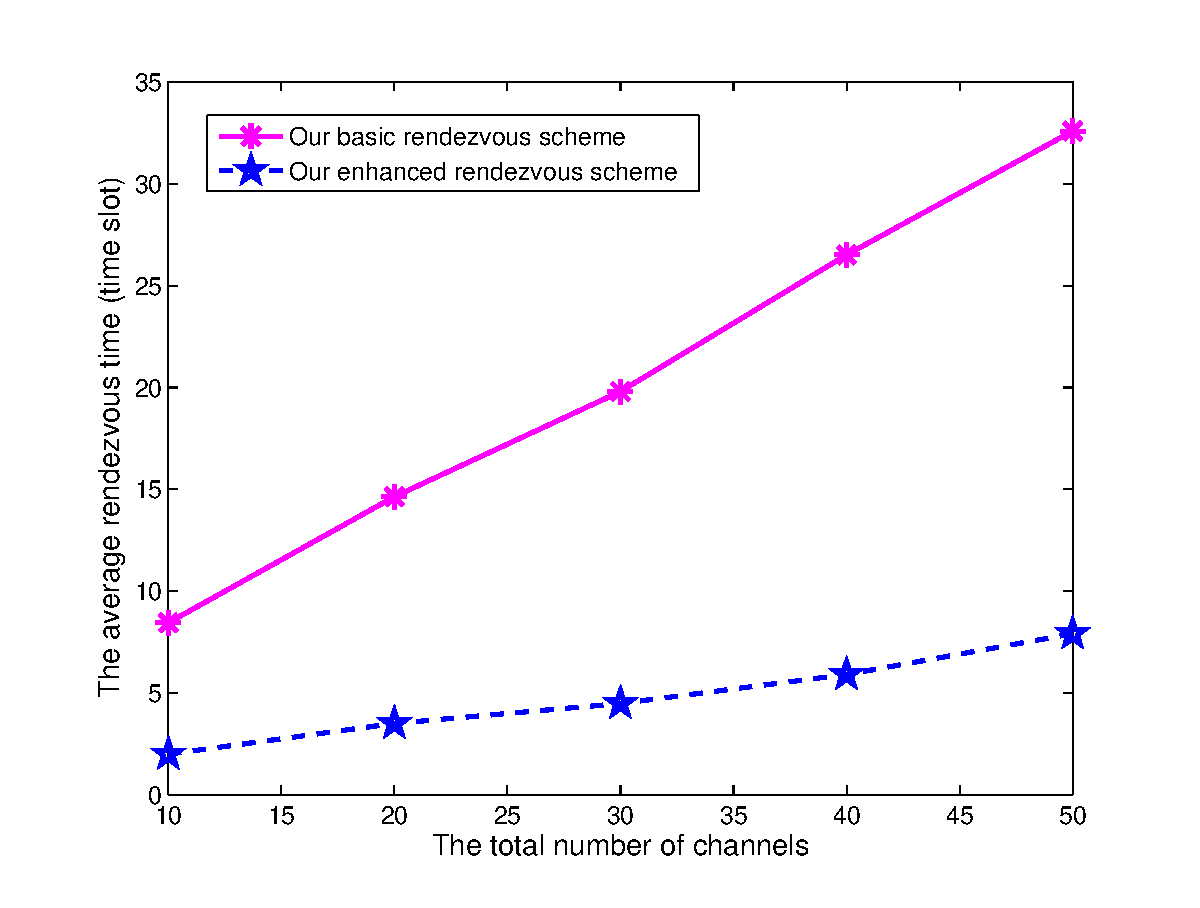
\includegraphics[width=10cm,height=8cm]{sec_3_2_rend1.eps} 
      \caption{The average rendezvous time as the total number of channel increases.}
    \label{sec_3_2_fig_rend1} 
    \end{center}   
\end{figure} 

In Fig. \ref{fig:rend11}, we shows the successful ratios of
the rendezvous of both the basic and enhanced rendezvous schemes. The successful
ratio is defined as the number of successful rendezvous to the total number
of performed rendezvous. According to the \textit{send-or-receive problem},
two SUs cannot achieve a successful rendezvous even when they hop the same
channel, if during that time slot they applied the same send-or-receive allocations,
which may cause collisions between RTS packets. Therefore, the successful
ratio of rendezvous is an important metric to evaluate a rendezvous scheme
considering the \textit{send-or-receive problem}. In Fig. \ref{fig:rend11},
the successful ratio of both scheme are very close to $100\%$, which means
they are very useful for practical implementations.

\begin{figure}[hbtp] 
    \begin{center} 
      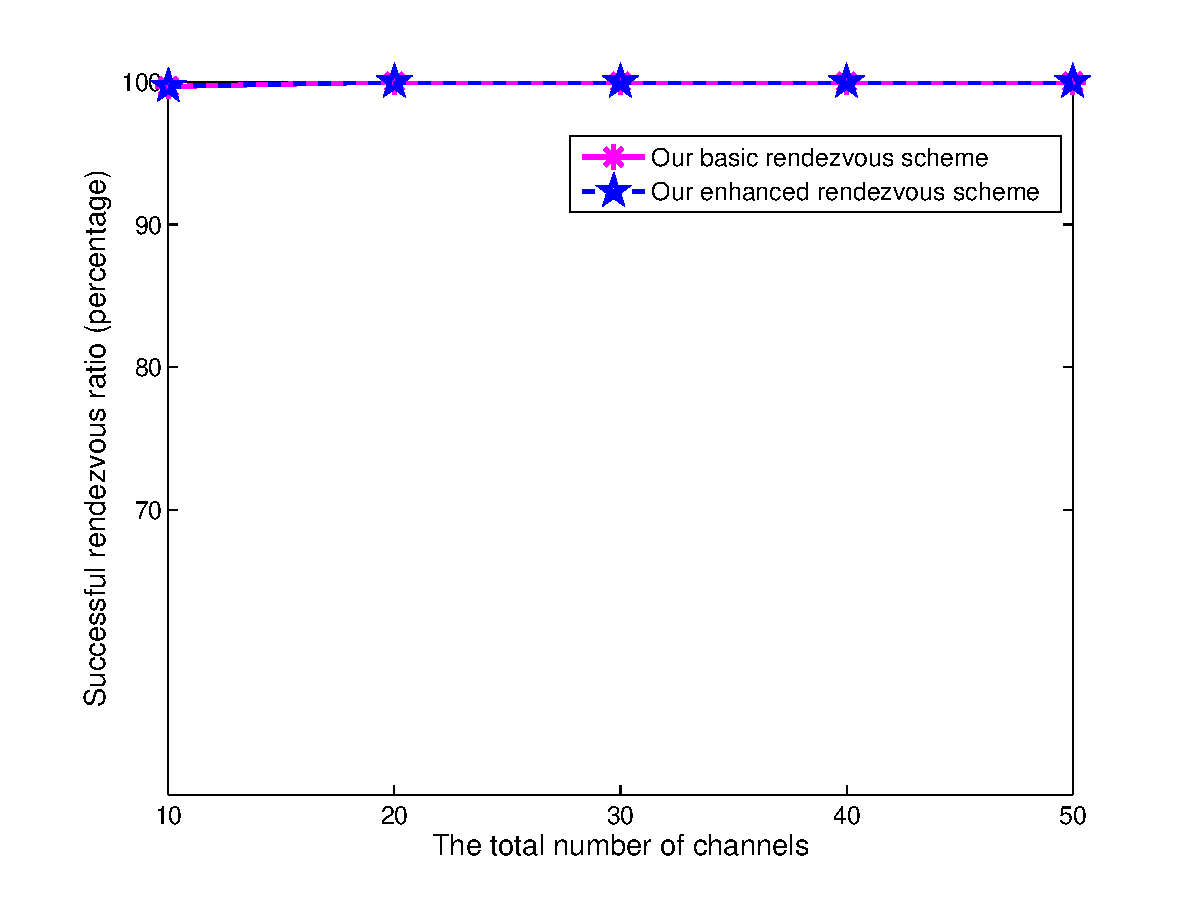
\includegraphics[width=10cm,height=8cm]{sec_3_2_rend11.eps} 
      \caption{The successful rendezvous ratio as the total number of channel increases.}
    \label{fig:rend11} 
    \end{center}   
\end{figure} 

% \begin{figure}[hbtp]
%        \centering
%    \subfigure[The average rendezvous time]{
%      \label{fig:rend1}
%      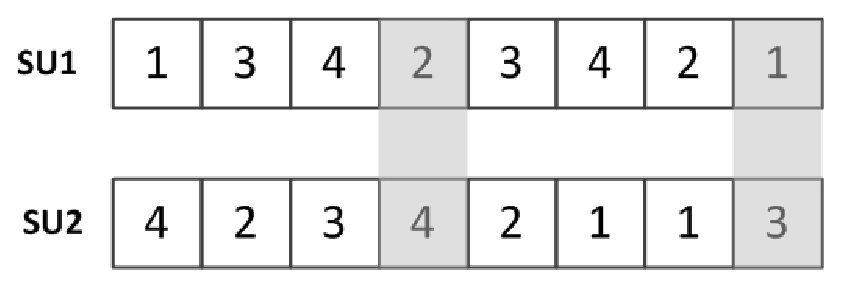
\includegraphics[width=4cm,height=5cm]{rend1.eps}
%    }
%    \subfigure[The successful rendezvous ratio]{
%      \label{fig:rend11}
%      \includegraphics[width=4cm,height=5cm]{rend11.eps} 
%    }
%        \caption{The impact from the total number of channel.}
%\end{figure}

\subsection{The impact of the channel available ratio}
In this part, we evaluate the impact of the channel available ratio which
is defined as the number of available channels of a SU to the total number
of channel. In the simulations,  we set $R = 4$, $M = 30$, and the channel
available ratio from $0.3$ to $0.9$. 

In Fig. \ref{fig:rend2}, we can notice
that both schemes result in lower rendezvous time as the channel available
ratio increases. This is because, with a higher channel available ratio,
the two schemes can utilize more channels to perform channel hopping and
RTS transmissions, which increases the probability of a successful \textit{link
rendezvous}.  Furthermore, the enhanced scheme always outperforms the basic
one, but when the channel available ratio increases, the difference between
the two schemes' results decreases. This is the reason that when the channel
available ratio increases, the difference between two schemes is less obvious,
since the main difference between the two schemes is that the enhanced one
can well utilize all the cognitive radios and the available channels.

\begin{figure}[hbtp] 
    \begin{center} 
      \includegraphics[width=10cm,height=8cm]{sec_3_2_rend2.eps} 
      \caption{The average rendezvous time as the channel available ratio increases.}
    \label{fig:rend2} 
    \end{center}   
\end{figure} 

Fig. \ref{fig:rend22} shows the successful rendezvous ratio of the two schemes
as the channel available ratio increases. We can notice that only when the
channel available ratio is $0.3$, the successful rendezvous ratio is a little
bit lower than $100\%$, while always $100\%$ when the value is higher than
$0.3$. Therefore, both of our proposed schemes can be applied in different
cognitive radio networks with different channel availability.

\begin{figure}[hbtp] 
    \begin{center} 
      \includegraphics[width=10cm,height=8cm]{sec_3_2_rend22.eps} 
      \caption{The successful rendezvous ratio as the channel available ratio increases.}
    \label{fig:rend22} 
    \end{center}   
\end{figure} 

% \begin{figure}[hbtp]
%        \centering
%        \subfigure[The average rendezvous time]{
%      \label{fig:rend2}
%      \includegraphics[width=4cm,height=5cm]{rend2.eps} 
%        }
%        \subfigure[The successful rendezvous ratio]{
%      \label{fig:rend22}
%      \includegraphics[width=4cm,height=5cm]{rend22.eps} 
%        }
%        %\label{fig:rend22}
%        \vspace{-0.2cm}
%        \caption{The impact of the channel available ratio.}
%\end{figure}

\subsection{The impact of the number of cognitive radios}
In this part, we evaluate the impact of the number of cognitive radios on
the average rendezvous time and the  successful rendezvous ratio. 

Fig. \ref{fig:rend3}
indicates that the enhanced scheme always outperforms the basic one when
the number of cognitive radios increases. However, the difference between
the results of the two schemes decreases as the number of cognitive radios
increases. This is because as the number of cognitive radios increases, each
SU can utilize more available channels during one time slot, therefore the
difference between the two schemes is not very obvious.

\begin{figure}[hbtp] 
    \begin{center} 
      \includegraphics[width=10cm,height=8cm]{sec_3_2_rend3.eps} 
      \caption{The average rendezvous time as the number of cognitive radio increases.}
    \label{fig:rend3} 
    \end{center}   
\end{figure} 


Fig. \ref{fig:rend33} shows the rendezvous successful ratio
of the proposed schemes as the number of cognitive radios of each SU increases.
We can notice that both proposed schemes can achieve $100\%$ successful ratio
as the number of cognitive radios of each SU changes from $2$ to $8$. The
results indicates that both of the proposed schemes can be applied to various
cognitive radio networks when SUs are equipped with multiple cognitive radios.

\begin{figure}[hbtp] 
    \begin{center} 
      \includegraphics[width=10cm,height=8cm]{sec_3_2_rend33.eps} 
      \caption{The successful rendezvous ratio as the number of cognitive radio increases.}
    \label{fig:rend33} 
    \end{center}   
\end{figure} 

% \begin{figure}[hbtp]
%        \centering
%        \subfigure[The average rendezvous time]{
%      \label{fig:rend3}
%      \includegraphics[width=4cm,height=5cm]{rend3.eps} 
%        }
%        \subfigure[The successful rendezvous ratio]{
%      \label{fig:rend33}
%      \includegraphics[width=4cm,height=5cm]{rend33.eps} 
%        }
%        %\label{fig:rend33}
%        \vspace{-0.2cm}
%        \caption{The impact of the number of cognitive radios.}
%\end{figure}

\subsection{The optimal channel allocation scheme}
In this section, we evaluate the optimal channel allocation scheme proposed
in Section \ref{sec:renWithInfo}. In the following simulations, we assume
there are $N_{c}$ SUs who know the locations
and current available channels information of each other. Furthermore, we
assume that some of a SU's radios have been allocated with available channels.
We try to optimally allocate available channels to the remaining free radios.
We call a channel allocation to a radio of a SU a valid allocation when no
 other SU, who are located in the SU's interference range, allocates the
same channel. Our goal is to maximize the total number of valid allocations
among the $N_{c}$ SUs. To the best of our knowledge, there is no existing
scheme considering this problem in multiple-radio rendezvous. Therefore,
we compare our proposed scheme with the random channel allocation scheme
in which a SU randomly chooses available channels for the rest free cognitive
radios.

Fig. \ref{fig:alloc1} shows the total number of valid allocations under the
two schemes when the total number of channels changes from $10$ to $50$.
In the simulations, we set $N_{c} = 8$, available channel  ratio as $0.5$,
and the number of cognitive radios $R = 8$. We can notice that our proposed
scheme always performs much better than the random allocation scheme, since
we consider the channel interference in allocations. Furthermore, the difference
between the two schemes is almost unchanged when the total number of channel
changes from $10$ to $50$.

\begin{figure}[hbtp] 
    \begin{center} 
      \includegraphics[width=10cm,height=8cm]{sec_3_2_alloc1.eps} 
      \caption{The number of free radios with valid allocations as the total
number of channels increases.}
    \label{fig:alloc1} 
    \end{center}  
\end{figure} 

Fig. \ref{fig:alloc2} shows the results when the  available channel ratio
changes from $0.3$ to $0.9$. We also set $N_{c} = 8$, the total number of
channels as $30$, and the number of cognitive radios $R = 8$. The results
show that our scheme always outperforms the random allocation scheme when
the available channel  ratio changes. Furthermore, the number of valid allocations
 of our proposed scheme is almost stable with different  available channel
ratios.

\begin{figure}[hbtp] 
    \begin{center} 
      \includegraphics[width=10cm,height=8cm]{sec_3_2_alloc2.eps} 
      \caption{The number of free radios with valid allocations as the available
channel ratio increases.} 
    \label{fig:alloc2} 
    \end{center}   
\end{figure} 

In Fig. \ref{fig:alloc3}, we show the simulation results as $N_{c}$ changes
from $3$ to $8$. Since $N_{c}$ changes in each simulation, we evaluate the
average number of valid allocations rather than the total number of valid
allocations. The results indicate that our proposed scheme outperforms the
random allocation scheme under different $N_{c}$. However, when $N_{c}$ increases,
the performance of both two schemes decreases. The reason is that when $N_{c}$
increases, the number of SUs within a SU's interference range may also increase,
which decreases the probability that a channel can be validly allocated for
the SU.

\begin{figure}[hbtp] 
    \begin{center} 
      \includegraphics[width=10cm,height=8cm]{sec_3_2_alloc3.eps} 
      \caption{The average number of valid allocations as $N_c$ increases.}
    \label{fig:alloc3} 
    \end{center}  
\end{figure} 

\chapter{Rendezvous Schemes Without Predetermined Send and Receiver Considering a Single Radio}
\label{chapter_single_radio}
In this chapter, we propose two efficient rendezvous schemes under the scenarios
that there is not a predetermined sender or receiver for a rendezvous process
during the initialization phase of cognitive radio networks when SUs are
equipped with single radio.
\section{System Model and Problem Description}
\label{sec_3_3_pro}
In this research, we assume that there are totally $N$ SUs and $N_{p}$ PUs coexisting. There are totally $M$ channels that all the SUs and PUs can access. Furthermore, each SU is equipped with a
half-duplex cognitive radio. Therefore, a cognitive radio cannot send and receive signals simultaneously. There is no CCC in the network through which all SUs can exchange their control information. Before the initialization process of a CRN, each SU does not know any control information about other SUs, which is a very practical assumption. A time-slotted system is deployed among all SUs and PUs  and they do no need to be strictly synchronized.

A channel hopping scheme is adopted for the  rendezvous process between two SUs. During a rendezvous process, each SU hops to the current  channel based on a channel hopping sequence, senses the current availability of the channel, and sends an RTS packet or waits for an RTS packet from another SU. Therefore, each time slot includes the sensing phase and the sending or receiving phase during the rendezvous process. According to existing rendezvous schemes, a successful  rendezvous occurs when  two SUs hop to a common available channel at the same time slot, but the process of sending an RTS packet and receiving a CTS reply is not considered. In this research we define this kind of rendezvous as  \textit{channel rendezvous}. This may not be a problem when one SU is always the sender while the other is the receiver, which means that there is an explicit send-or-receive relationship between the two SUs. Under this scenario, after one SU sends an RTS packet,  if the other SU receives the RTS packet and replies a CTS packet, the rendezvous succeeds.

However, during the initialization phase of a CRN, each SU may try to rendezvous with other SUs to exchange control information. There is no explicit role for an SU, since it cannot know if other SUs are senders or receivers currently. If two SUs hop to a common available channel and their transceivers are both tuning to the sending mode , none of them can receive the RTS packets, which can fail a successful rendezvous. Furthermore, each SU does not know if its target SU is on the current common available channel and is  in the sending or receiving mode  during the current time slot. Practically, only when the two SUs hop to a common available channel and when one SU is sending  while the other is trying to receive on that channel, a successful rendezvous can finally happen. In this research, we denote this kind of rendezvous as  \textit{link rendezvous}. Therefore, in a \textit{link rendezvous} process without the explicit sender or receiver , an SU  should not only determine the channel it should hop to but also whether tuning its half-duplex radio to the sending or receiving mode during a time slot. We call this problem as the \textit{send-or-receive problem} in a \textit{link rendezvous} scheme.

For the $i$th SU, during time slot $t$ of a link rendezvous process, it generates a \textit{task allocation} $\mathbb{A}^{t}_{i} = (c^{t}_{i}, s^{t}_{i})$, where $1\leq c^{t}_{i} \leq M$, $s^{t}_{i} = 1$ (send) or $s^{t}_{i} = 0$ (receive).  We also denote $C_{i}^{t}$ as the available channel set of the $i$th SU during  time slot $t$. We define  \textit{link rendezvous} as follows.

\textit{Link Rendezvous}: A successful link rendezvous between the $i$th SU and the $j$th SU during time slot $t$ requires that $(c^{t}_{i}, s^{t}_{i})$ and $(c^{t}_{j}, s^{t}_{j})$ satisfy $c^{t}_{i} \in C^{t}_{i}$, $c^{t}_{j} \in C^{t}_{j}, c^{t}_{i} = c^{t}_{j}$, and $s^{t}_{i}\ \mbox{XOR}\ s^{t}_{j} = 1$.

In the following two sections, we propose two different distributed link rendezvous schemes based on two different basic ideas.
\section{The Basic Link Rendezvous Scheme}
\label{sec:ba_rend}
Our basic idea is that besides the channel hopping sequence, considering the send-or-receive problem,  there is a  \textit{transmission sequence}
$S_i$ for the $i$th SU. $S_i$ only contains $0$ or $1$ values which represent
the sending mode or receiving mode, respectively,  for each SU during each time slot, i.e, If $S_i[t] = 1$,
during the current time slot, the SU should tune its transceiver to the
sending mode, and If $S_i[t] = 0$, during the current time slot, the SU should tune its transceiver to the receiving mode. When tuning to the sending
mode during a time slot, an SU can first send an RTS packet on the current channel and
then tune to the receiving mode waiting for a replied CTS packet. When tuning to the receiving mode, an SU should tune the transceiver to the receiving mode, wait for RTS packets from  other SUs on the current channel, and tune to the sending to reply a CTS packet if it received an RTS packet.

Since we try to design a distributed scheme for each SU, our idea for the basic link rendezvous scheme is to make each SU apply the same  basic transmission sequence $S_b$.
We assume that the length of the  basic transmission sequence $S_b$ is $L$ and each SU circularly hops according to $S_b$, i,e, if the SU hops to the end of $S_b$, it should hop to the first element of $S_b$ during the next time slot.  For example, if the  transmission sequence is $\{1,0,0,1\}$,
the real transmission sequence should be $\{1,0,0,1,1,0,0,1,1,0,0,1\dots\}$. However, since
two SUs are not synchronized and do not know any control information about each other
before a successful link rendezvous, two SUs may follow different  real transmission
sequences even though they all follow the same basic transmission sequence $S_b$. Therefore, for the $i$th SU and $j$th SU, the real transmission
sequence of the $j$th SU $S_j$ should be a circular shift from the $i$th
SU's real transmission sequence $S_{i}$. For example, if the basic transmission sequence $S_b$
is $\{1,0,0,1\}$, $S_{i}$ is $\{1,0,0,1,1,0,0,1,\dots\}$, and $S_{j}$ is $\{1,1,0,0,1,1,0,0,\dots\}$.

We define the element pair $(S^{t}_i, S^{t}_j)$ as the \textit{transmission pair}
of the $i$th and $j$th SU. According to the previous analysis, only when one SU is on sending mode while the
other is on receiving mode, two SUs can successfully finish a RTS and CTS
exchange. Therefore, only the transmission pair $(0,1)$ or $(1,0)$ can result
in a successful link rendezvous. We define $(0,1)$ or $(1,0)$ as the \textit{valid transmission
pair}.  We define the \textit{valid number} $N_v = \mathcal{V}(S_{i},
S_{j})$ as the number  of valid transmission pairs two real transmission
sequences could get within the period $L$, where
\begin{equation}
 \mathcal{V}(S_{i}, S_{j}) = \sum_{k=0}^{L-1}[(S_{i}[k]\ XOR\ S_{j}[k])
== 1].
\end{equation}
Furthermore, the average valid number $\overline{N_v}$ of a basic transmission
sequence $S_b$  is defined as
\begin{equation}
\overline{N_v} = \mathcal{B}(S_b)=\DF{1}{L}\sum_{k=0}^{L-1}\mathcal{V}(S_{i},
\mathcal{H}(S_j, k)),
\end{equation}
where $\mathcal{H}(S_j, k)$ is defined as the function to make $S_j$ perform
$k$ times circularly left shifts. A larger $\overline{N_v}$ means that there are more valid transmission pairs within a period which can make a successful link rendezvous happen with a higher probability. Therefore, our goal is to find the optimal
basic transmission sequence $S_b$ for a given length $L$, which can finally result in 
the largest average valid number $\overline{N_v}$.

To get the optimal basic transmission sequence $S_b$ with length $L$, we first derive the following lemma:
\begin{lemma}
\label{le:valid1}
For a basic transmission sequence with length $L$, if there are $n$ $1$ elements
in it. The average valid number $\overline{N_v}$ is $2(nL-n^2)/L.$
\end{lemma}
\begin{proof}
Considering all the $L$  scenarios regarding different circular shifts regarding a basic transmission sequence, each $1$ element can generate total
$L-n$ such $(1,0)$ pairs which are valid transmission pairs. Therefore there are total $2n(L-n)$ $(1,0)$ pairs two basic transmission sequences can get. Finally,
the average valid number considering all $L$ different circular shifts 
is    
$2(nL-n^2)/L$.
\end{proof}

\begin{lemma}
\label{le:optimal1}
When the number of $1$  elements in $S_b$ is $\DF{L}{2}$, The average valid number
$\overline{N_v}$ reaches its maximum value $L/2$.
\end{lemma}
\begin{proof}
For a given $L$, $\overline{N_v} = \DF{2}{L}(n_rL-n_r^{2}) = \DF{2}{L}(-(n_r-\DF{L}{2})^{2}+\DF{L^{2}}{4})$.
Therefore, when $n=\DF{2}{L}$, $\overline{N_v}$ reaches the maximum value
$\DF{2}{L}\times \DF{L^2}{4} = \DF{L}{2}$.
\end{proof}

\textbf{Lemma \ref{le:valid1}} indicates that $\overline{N_v}$ is only related
to the number of $1$ elements in $S_b$ regardless of their positions, for a given
$L$. Therefore,  each SU can just generate its own basic transmission sequence of length $L$ which also should contains $\DF{L}{2}$ $1$ elements. We propose a distributed  algorithm for each SU to achieve a successful link rendezvous in \textbf{Algorithm \ref{al:rend1}} in which we let $L$ equal to the number of total channels.
\begin{algorithm} 
  \caption{The basic distribute rendezvous algorithm for each SU}
  \begin{algorithmic}[1] 
  \label{al:rend1}
    \REQUIRE ~~\\
    The total number of channels: $M$\\
    A channel hopping sequence: $S$\\
    
    \STATE Randomly generate a basic transmission sequence $S_b$ with length $M$;
    \STATE Randomly choose a starting index $i$ on $S_b$;
    \STATE $count=0$; //count time slots
    \WHILE{Not rendezvous}
         \STATE Hop to the current channel according to $S$.
         \IF{the current channel is available and $S_b[i]==1$}
            \STATE Tune to the sending mode
and send RTS packets;         \ENDIF
         \IF{the current channel is available and $S_b[i]==0$}
            \STATE Tune to the receiving mode;
         \ENDIF
         \STATE i++;
         \IF{$i>M$}
             \STATE i = 1; //circularly hop
         \ENDIF
    \ENDWHILE
  \end{algorithmic}
\end{algorithm} 

Here is an example of the basic link rendezvous scheme in Fig. \ref{fig:rend-basic}, where $M = 4$, the transmission sequence of SU1 is $\{1,0,0,1\}$, the transmission sequence of SU2 is $\{1,1,0,0\}$, each SU hops according to its own channel hopping sequence, and the common available channels for them are channel $3$ and $2$. The two SUs first hop to the common available channel $3$. However, they do not achieve a successful link rendezvous since they are all tuning to the sending mode during that time slot. Therefore, they just continue the channel hopping process until they all hop to the common available channel $2$. Finally, they achieve a successful link rendezvous on channel $2$ since SU1 is tuning to the sending mode and SU2 is tuning to the receiving mode.
\begin{figure}[hbtp] 
    \begin{center} 
        \includegraphics[width=12cm,height=4cm]{sec_3_3_rend-basic.eps}
        \caption{An example of the basic link rendezvous scheme.} 
        \label{fig:rend-basic}
    \end{center} 
\end{figure} 

Based on \textbf{Algorithm \ref{al:rend1}}, we can get the following theorem:

\addtocounter{theorem}{-2}
\begin{theorem}
\label{sec_3_3_theorem_exp_t}
The expectation of time slots to achieve a link rendezvous for \textbf{Algorithm \ref{al:rend1}}
is $E[T]=2T_e$, where $T_e$ is the expectation of the channel rendezvous time for a specific given channel hopping sequence.
\end{theorem}
\begin{proof}
According to the design of the transmission sequence of each SU, the probability that there is one sender and one receiver when two SUs hop to a common available channel is $0.5$, Therefore, if two SUs hop to a common available channel, the probability of a successful link rendezvous is $0.5$. If a link rendezvous fails because of that there is not a valid transmission pair, two SUs should continue the channel hopping process until a successful link rendezvous. Finally, the expectation of time slots to achieve a link rendezvous time is:
\begin{equation}
\sum_{i=1}^{\infty} T_e(1-0.5)^{(i-1)}(0.5) = \DF{T_e}{0.5} = 2T_e.
\end{equation}
\end{proof}
\section{The Enhanced Link Rendezvous Scheme}
\label{sec:en_rend}
In the basic link rendezvous scheme, each SU should follow two sequences, the channel hopping sequence and the transmission sequence. In this section,  we propose an enhanced link rendezvous scheme that each SU can just follow a \textit{virtual channel hopping sequence} so each SU does not need to implement an existing channel hopping sequence and a transmission sequence simultaneously.

Our basic idea is to combine the channel hopping sequence with the transmission sequence. Therefore, we expand the total $M$ practical channels to $2M$ \textit{virtual channels}.
For real channel $i$, we map it to two virtual channels $i$ and $i+M$. An example of generating the virtual channels when $M$ equals $4$ is shown in Fig. \ref{fig:virtual}. Therefore,
after this mapping process, for each SU, there are total $2M$ virtual channels.
Each SU hops according to a \textit{virtual channel hopping sequence} generated from the total $2M$ virtual channels. When an SU hops to the virtual channel $i$ that $i \leq M$, it should tune
its transceiver to the sending mode and hop to real channel $i$. On the other
side, when an SU hops to the virtual channel $i$ that $M<i\leq 2M$, it should tune its transceiver
to the receiving mode and  hop to real channel $i-M$. Furthermore, if channel
$i$ is available to an SU during current time slot, both  virtual channels $i$ and $i+M$
are also available to the SU.

\begin{figure}[hbtp] 
    \begin{center} 
        \includegraphics[width=8cm,height=4cm]{sec_3_4_virtual.eps} 
        \caption{An example of generating virtual channels.} 
        \label{fig:virtual}
    \end{center} 
\end{figure} 

Therefore, based on the virtual channel hopping sequence and 
the send-or-receive problem, a successful link rendezvous is defined as follows: %%%add a figure to show an example of virtual channel

\textit{Successful link rendezvous}: During time slot $t$, if the $i$th SU
hops to the virtual channel $c^{t}_i$ and the $j$th SU hops to the virtual channel
$c^{t}_j$, a successful link rendezvous is achieved if $|c^{t}_i-c^{t}_j|
= M$, $c^{t}_i\in \mathcal{C}^{t}_i$, and $c^{t}_j\in \mathcal{C}^{t}_j$,
where $\mathcal{C}^{t}_i$ and $\mathcal{C}^{t}_j$ are the current available
virtual channel sets of the $i$th and $j$th SU, respectively.

According to the definition of a successful link rendezvous based on the virtual channel hopping sequence, it is quite different from a successful \textit{channel rendezvous} that two SUs hop to a common available channel at the same time slot. Therefore, all the existing channel hopping sequences which can guarantee a successful \textit{channel rendezvous} cannot achieve a successful \textit{link rendezvous}  based on the virtual channels.

Our goal in this section is to design an efficient \textit{link rendezvous} scheme which
can achieve a fast successful link rendezvous between two SUs. The first step is to design a virtual channel hopping sequence based
on the total $2M$ virtual channels. The basic idea about the virtual channel hopping
sequence is to make each SU performs channel hopping according to the same
virtual channel hopping sequence $\mathcal{S}$ generated from $2M$ virtual channels. However,  since two SUs are fully distributed and
not synchronized, even though they follow the same virtual channel hopping sequence,
they may stay on the different positions of it. Therefore, the
sequence should try to achieve a successful link rendezvous regardless of different
positions of two SUs on the same virtual channel hopping sequence.

The first step to generate such a virtual channel hopping sequence is to generate a basic
sequence $\mathcal{B}$ such that its length is $4M$ and $\mathcal{B}[i]=\mathcal{B}[j]
= j-i, 1\leq i<j\leq 4M$, for any $1\leq\mathcal{B}[i]\leq 2M$, where $\mathcal{B}[i]$ is
the $i$th element of $\mathcal{B}$. Therefore, each number in the range $[1,M]$
appears exactly twice in $\mathcal{B}$.


Based on the definition of $\mathcal{B}$, we can first get the following
lemma regarding the existence of $\mathcal{B}$.

\addtocounter{theorem}{1}
\begin{lemma}
\label{lemma:guar_rend1}
If two SUs follow the same basic virtual channel hopping sequence $\mathcal{B}$, the first SU starts from the $i$th element , the second SU
starts from the $j$th element, and $k=|i-j|>0$, they could both hop to 
 virtual channel $k$ if $k\leq 2M$, or virtual channel $4M-K$ if $2M<k<4M$, within $4M$ time slots.
\end{lemma}
\begin{proof}
According to the definition of $\mathcal{B}$, if $k\leq 2M$, there are two
elements in the sequence $\mathcal{B}[u]=\mathcal{B}[v]=k, v > u$, and $|v-u|=k$.
Therefore, the two SUs can all hop to the virtual channel $k$ within $4M$
time slots. If $2M<k\leq 4M$, since two SUs hop according to the same $\mathcal{B}$
circularly, the distance between them on the sequence is also $4M-K < 2M$.
Therefore, according to the definition of $\mathcal{B}$, there are two elements
in the sequence $\mathcal{B}[u]=\mathcal{B}[v]=4M-k, v > u$, and $|v-u|=4M-k$.
\end{proof}

Here is an example in Fig.\ref{fig:rend0}. In the example, we assume that $M=2$, SU1 starts from the first channel in $\mathcal{B}$, and  SU2 starts from the fourth channel in $\mathcal{B}$, during the fifth time slot, both SUs   hop to channel $3$.

\begin{figure}[hbtp] 
    \begin{center} 
        \includegraphics[width=12cm,height=3cm]{sec_3_3_rend0.jpg} 
        %\vspace{-0.4cm}
        \caption{An example of the basic virtual channel hopping sequence.} 
        \label{fig:rend0}
    \end{center} 
\end{figure}

To get the final virtual channel hopping sequence $\mathcal{S}$, The second step
is to replace some elements in $\mathcal{B}$
according to the following manipulations: for each number $k$ that $\mathcal{B}[i]=\mathcal{B}[j]=k,
1\leq i<j\leq 4M$, if $k \leq M$, reset $\mathcal{B}[j] = k+M$, otherwise
reset $\mathcal{B}[j] = k-M$. An example is shown in Fig. \ref{fig:replace}, where $M=2$ and the basic sequence $\mathcal{B}$
could be $\{1,1,4,2,3,2,4,3\}$, after the replacements, the final channel
hopping sequence $\mathcal{S}$ should be $\{1,3,4,2,3,4,2,1\}$.
\begin{figure}[hbtp] 
    \begin{center} 
        \includegraphics[width=12cm,height=3cm]{sec_3_3_replace.eps} 
        \caption{An example of the replacement manipulations.} 
        \label{fig:replace}
    \end{center} 
\end{figure}

In order to generate the virtual channel hopping sequence $\mathcal{S}$, we have the following lemmas about some important features of the basic virtual channel hopping sequence $\mathcal{B}.$

\begin{lemma}
\label{lemma:noexist}
When $2M\ mod\ 4=2$, $\mathcal{B}$ does not exist.
\end{lemma}
\begin{proof}
According to the definition of $\mathcal{B}$, designing the basic
sequence is equivalent to dividing all the indexes $1,2,\dots, 4M$, these $4M$ numbers into
two lists $\mathcal{L}_{1}$ and $\mathcal{L}_{2}$, each of which has exactly
$2M$ different numbers, such that for $k=1,2,\dots,2M$, $\mathcal{L}_{2}[k]
- \mathcal{L}_{1}[k] = k$. Then, we have
        \begin{equation}
        \label{sec_3_3_eq_sum1}
        \sum^{2M}_{k=1}\mathcal{L}_{2}[k]-\sum^{2M}_{k=1}\mathcal{L}_{1}[k]=\sum^{2M}_{k=1}k=\DF{2M(2M+1)}{2},
        \end{equation}
        \begin{equation}
        \label{sec_3_3_eq_sum2}
        \sum^{2M}_{k=1}\mathcal{L}_{2}[k]+\sum^{2M}_{k=1}\mathcal{L}_{1}[k]=\sum^{4M}_{k=1}k=2M(4M+1).
        \end{equation}
        Combining \eqref{sec_3_3_eq_sum1} and \eqref{sec_3_3_eq_sum2}, we can get 
        \begin{equation}
        \label{sec_3_3_eq_sum3}
        \sum^{2M}_{k=1}\mathcal{L}_{2}[k]=\DF{10M^{2}+3M}{2}.
        \end{equation}
        When $2M\ mod\ 4=2$, $M$ is an odd number that can be represented as $M=2e+1, e\geq 0$, thus
        \begin{equation}
        \label{eq:sum4}
        \sum^{2M}_{k=1}\mathcal{L}_{2}[k]=\DF{10(2e+1)^{2}+3(2e+1)}{2}=20e^2+23e+\DF{13}{2}.
        \end{equation}
        
 the right-hand side of \eqref{eq:sum4} is not an integer which contradicts the fact that it is a sum of $4M$ integers.
\end{proof}
     
\begin{lemma}
\label{sec_3_3_lemma_exist}
When $M>1$ and $2M\ mod\ 4=0$, $\mathcal{B}$ exists.
\end{lemma}
\begin{proof}
        When $M=2$, sequence $\{1,1,4,2,3,2,4,3\}$ satisfies the requirements
of our desired basic link rendezvous sequence.
        When $M>2$, the proof can be found in the second page of \cite{tSkolem57OCDOI}.
\end{proof}

Based on the proof of \textbf{ Lemma \ref{lemma:noexist}} and \textbf{ Lemma
\ref{sec_3_3_lemma_exist}}, we propose \textbf{Algorithm \ref{sec_3_3_algorithm_generate}} to generate
our virtual channel sequence $\mathcal{S}$.

\begin{algorithm} 
  \caption{The algorithm for generating the virtual channel hopping sequence}
  \begin{algorithmic}[1] 
  \label{sec_3_3_algorithm_generate}
    \REQUIRE ~~\\
    The number of channels : $M$
    \ENSURE ~~\\
    The desired rendezvous sequence: $\mathcal{S}$\\
    \STATE $n = 2M$;
    \IF{$n\%4==2$}
        \STATE $n = n+2$;
    \ENDIF
    \IF{$n==4$}
         \STATE $\mathcal{S}=\{1,1,4,2,3,2,4,3\}$;
    \ELSE
        \STATE Initialize $\mathcal{S}$ as a list of length $4n$;
        \STATE Let $P$ be an empty list;
        \STATE $m=\lfloor n/4 \rfloor$;
        \STATE Add all pairs $(4m+r, 8m-r)$, for $r=0,1,\dots,2m-1$, to $P$;
        \STATE Add pairs $(2m+1, 6m)$ and $(2m, 4m-1)$ to $P$;
        \STATE Add all pairs $(r, 4m-1-r)$, for $r=1,3,\dots,m-1$, to $P$;
        \STATE Add pair $(m, m+1)$ to $P$;
        \STATE Add all pairs $(m+2+r, 3m-1-r)$, for $r=0,1,\dots,m-3$, to $P$;
    \FOR{$i=1$ to $n$}
        \STATE $\mathcal{S}[P[i].first] = \mathcal{S}[P[i].second] = P[i].second
- P[i].first$;
    \ENDFOR
    \ENDIF
    \FOR{$i=1$ to $2n$}
        \IF{$\mathcal{S}[i] > 2M$}
             \STATE $\mathcal{S}[i]\ \% = 2M$; //limit each value to $[1,2M]$
        \ENDIF
    \ENDFOR
    \FOR{$i=1$ to $2n$}
        \STATE //replacement manipulations
        \IF{this the second time that $k=\mathcal{S}[i]$ appears}
             \IF{$k \leq M$}
                  \STATE $\mathcal{S}[i] = \mathcal{S}[i] + M;$
             \ENDIF
             \IF{$k > M$}
                  \STATE $\mathcal{S}[i] = \mathcal{S}[i] - M;$
             \ENDIF
        \ENDIF
    \ENDFOR
    \RETURN $\mathcal{S}$;
  \end{algorithmic}
\end{algorithm} 

According to \textbf{Algorithm \ref{sec_3_3_algorithm_generate}}, if $M>0$ and $2M\ mod\ 4=2$, the length of $\mathcal{S}$ should be larger than $4M$ in order to
guarantee the existence of $\mathcal{S}$. Furthermore, we have the following
lemma about $\mathcal{S}$ regarding a successful link rendezvous. After getting
the virtual channel hopping sequence $\mathcal{S}$, we can get the
following lemma regarding a  successful link rendezvous:

\begin{lemma}
\label{lemma:guar_rend2}
Assume that when a link rendezvous process begins, the first SU is on $i$th element of
$\mathcal{S}$, the second SU is on the $j$th element of $\mathcal{S}$, and
$k=|i-j|>0$. Within $4M$ time slots, two SUs can hop to two different virtual
channels
$c_1$ and $c_2$ such that $|c_1-c_2|=M$. 
\end{lemma}
\begin{proof}
According to \textbf{Lemma \ref{lemma:guar_rend1}}, within $4M$ time slots,
two SUs can hop to the same virtual channel $c$ on the different positions
of $\mathcal{B}$. Since we perform the replacement manipulations of $\mathcal{B}$
to get $\mathcal{S}$,  the manipulation can make the same two $c$ values
in $\mathcal{B}$ change to two different values $c_1$ and $c_2$ such that
$|c_1-c_2|=M$. Therefore, within $4M$ time slots,  two SUs can hop to two
different virtual channels $c_1$ and $c_2$ such that $|c_1-c_2|=M$.
\end{proof}

An example of Lemma \ref{lemma:guar_rend2} is shown in Fig. \ref{sec_3_3_fig_rend1}, where $M = 2$, the virtual channel sequence is $\{1, 3, 4, 2, 3, 4, 2, 1\}$, SU1 starts from the first element, and SU2 starts from the third element. Within $4M = 8$ time slots, two SUs first hop to channel $2$ and $4$ that $4-2 = 2 = M$ during the fourth time slot, and then hop to channel $1$ and $3$ that $3-1 = 2 = M$ during the eighth time slot.

\begin{figure}[hbtp] 
    \begin{center} 
        \includegraphics[width=12cm,height=3cm]{sec_3_3_rend1.jpg} 
        %\vspace{-0.4cm}
        \caption{An example of the virtual channel hopping sequence.} 
        \label{sec_3_3_fig_rend1}
    \end{center} 
\end{figure}

Since a necessary condition for a successful link rendezvous is that two SUs
should hop to two virtual channels $c_1$ and $c_2$, respectively, such that
$c_1>c_2, c_1-c_2=M$, we can design a channel hopping scheme based on \textbf{Lemma 6}. However, the problem is that if the virtual channel $c_2$
is not a common available virtual channel, the two SUs still cannot achieve
a successful rendezvous, even if they hop to $c_1$ and $c_2$
during the same time slot. Therefore, after every $4M$ time slots, if two SUs did
not achieve a successful link rendezvous, each SU should restart a new virtual channel
hopping process from a new starting element in $\mathcal{S}$ to make the two SUs
can hop to new virtual channels $c^{'}_1$ and $c^{'}_2$, respectively, until $c^{'}_2$ is a common available virtual channel. Therefore,
we design the following distributed link rendezvous scheme  for each SU in \textbf{Algorithm \ref{al:rend2}}:
\begin{algorithm} 
  \caption{The distribute link rendezvous algorithm for each SU}
  \begin{algorithmic}[1] 
  \label{al:rend2}
    \REQUIRE ~~\\
    The total number of channels: $M$\\

    \STATE Generate the virtual channel hopping sequence $\mathcal{S}$;
    \STATE Randomly choose a starting index $i$ on $\mathcal{S}$;
    \STATE $count=0$;// count time slots
    \WHILE{Not rendezvous}
         \IF{$\mathcal{S}[i] > M$ and $\mathcal{S}[i]$ is currently available}
            \STATE Hop to channel $\mathcal{S}[i]-M$ and tune to the receiving
mode;
         \ENDIF
         \IF{$\mathcal{S}[i] \leq M$  and $\mathcal{S}[i]$ is currently available}
            \STATE Hop to channel $\mathcal{S}[i]$, tune to the sending
mode,
and send RTS packets on the channel;        \ENDIF
         \STATE count++;
         \IF{$count >= 4M$}
            \STATE $count = 0$;
            \STATE Randomly generate a new $i$;//reset $i$
         \ELSE
            \STATE $i++$;
            \IF{$i>4M$}
                \STATE $i = 1$;//circular hop
            \ENDIF
         \ENDIF
    \ENDWHILE
  \end{algorithmic}
\end{algorithm}  

Based on \textbf{Algorithm\ref{al:rend2}}, we can get the following lemma:
\begin{lemma}
The probability that two SUs fail to rendezvous within every $4M$ time slots
is $p_f\approx 1-p_c$, where $p_c$ is the probability that a channel is a
common available channel of the two SUs. 
\end{lemma}
\begin{proof}
The probability that two SUs choose different starting indexes in $\mathcal{S}$
is $\DF{4M(4M-1)}{(4M)^2}=\DF{4M-1}{4M}$. Two SUs can achieve a  successful
link rendezvous only when they choose different starting indexes and the virtual 
channel they will hop to is available to both of them. Therefore, the probability
that two SUs achieve a successful rendezvous during every $4M$ time slots
is $\DF{4M-1}{4M}p_c$. Finally, the fail probability is $1-\DF{4M-1}{4M}p_c=\DF{4M-4Mp_c-p_c}{4M}=\
1-p_c-\DF{p_c}{4M}\approx 1-p_c$
\end{proof}

Finally, we can get the \textbf{Theorem \ref{sec_3_3_theorem_exp_t_2}} regarding the average link rendezvous time of the enhanced link rendezvous scheme in \textbf{Algorithm\ref{al:rend2}}.\addtocounter{theorem}{-6}
\begin{theorem}
\label{sec_3_3_theorem_exp_t_2}
The expectation of link rendezvous time slots for \textbf{Algorithm\ref{al:rend2}}
is $E[T]=\DF{4M}{p_c}$, where $M$ is the total number of channels and $p_c$
is the probability that a channel is a common available channel of the two
SUs.
\end{theorem}
\begin{proof}
The expectation of link rendezvous time slots is:
\begin{equation}
\sum_{i=1}^{\infty} 4Mp_{f}^{(i-1)}(1-p_f) = \DF{4M}{1-p_f} = \DF{4M}{p_c}.
\end{equation}
\end{proof}

\section{Performance Evaluations}
In this section, we show simulation results regarding our proposed link rendezvous
schemes under a practical CRN.  In our simulations, we assume that there
are two SUs and $N_p$ PUs coexisting. During each time slot, each SU hops
to a channel according to a channel hopping sequence. If a PU within the
SU's sensing range is using the channel, the SU cannot perform rendezvous
on this channel and should wait for the next time slot. For a PU, if there
are data packets in the queue waiting for transmitting, it just randomly
chooses a channel from channel $1$ to channel $M$. Otherwise, it just keeps
silent and waits for the next data packet. We assume that the data packet
arrival rate of each PU obeys Poisson distribution. The main parameters in
our simulations are shown in Table \ref{sec_3_3_table_parameters}.
\begin{table}[htb]
\caption{Simulation Parameters} 
\centering 
\begin{tabular}{|l|c|} 
\hline 
Side length of the simulation area $L$ & 200m\\ 
\hline 
The distance between the two SUs & 60m\\ 
\hline 
The transmission range of each SU & 80m\\
\hline 
The sensing range of each SU & 100m\\ 
\hline 
The Number of PUs: $N_{p}$ & 20 \\ 
\hline 
The Number of channels: $M$ & 20 \\ 
\hline 
The length of each time slot & 2ms\\ 
\hline 
The total number of time slots in a simulation: $T$ & 50000\\ 
\hline 
The length of a PU packet & 100 slots\\ 
\hline 
The PU packet arrival rate $\lambda_{p}$ & 5 per second\\ 
\hline 
\end{tabular} 
\label{sec_3_3_table_parameters} 
\end{table}

\subsection{Average Link Rendezvous Time Under Different Scenarios}
To the best of our knowledge, there are no existing rendezvous schemes considering
the link rendezvous problem. Therefore, in this paper, we compare the performance
of our proposed link rendezvous scheme with the random scheme that each SU
randomly chooses to send or receive during each time slot. As the random
scheme should work on an existing channel hopping sequence, in the simulations,
we apply the channel hopping sequence in \cite{jLi14ANCFF} which has similar
features with the virtual channel hopping sequence we propose in the enhanced
link rendezvous scheme.

Fig. \ref{fig:t_M} shows the average link rendezvous time of the random scheme
and the proposed scheme when the total number of channels $M$ increases from
$10$ to $50$. In the simulations, we set the number of PUs as $20$ and the
average packet of each PU as $1$ packet per second. The results indicate
that the proposed scheme outperforms the random scheme when the total number
of channels increases from $10$ to $50$. We can also notice that the average
link rendezvous time almost has a linear relation with the total number of
channels under the proposed scheme, which coincide the analysis in \textbf{Theorem
\ref{sec_3_3_theorem_exp_t_2}}.

\begin{figure}[hbtp] 
    \begin{center} 
      \includegraphics[width=10cm,height=8cm]{sec_3_3_t_M.eps} 
      \caption{The average link rendezvous time as the total number of channels increases.}
    \label{fig:t_M} 
    \end{center}   
\end{figure} 

Fig. \ref{fig:t_pu} shows the average link rendezvous time of the random
scheme
and the proposed scheme when the total number of PUs increases from
$10$ to $50$. In the simulations, we set the total number of channels as
$30$ and the average packet of each PU as $1$ packet per second. The results
indicate
that the proposed scheme outperforms the random scheme when the total number
of PUs increases from $10$ to $50$. We can also notice that the results under
the enhanced scheme change  less than the results under the random scheme,
which indicate that the enhanced scheme is more adaptable to various networking
conditions.

\begin{figure}[hbtp] 
    \begin{center} 
      \includegraphics[width=10cm,height=8cm]{sec_3_3_t_pu.eps} 
      \caption{The average link rendezvous time as the total number of PUs increases.}
    \label{fig:t_pu} 
    \end{center}   
\end{figure} 

% \begin{figure}[hbtp]
%      \centering
%      \subfigure[The average link rendezvous time as the total number of
%channels increases]{
%      \label{fig:t_M}
%      \includegraphics[width=4cm,height=4.8cm]{t_M.eps}
%      }
%      \subfigure[The average link rendezvous time as the total number of
%PUs increases]{
%      \label{fig:t_pu}
%      \includegraphics[width=4cm,height=4.8cm]{t_pu.eps} 
%      }
%     \vspace{-0.2cm}
%     \caption{The average link rendezvous time.}
%\end{figure}

\subsection{Link Rendezvous Successful Ratio}
In this section, we evaluate the successful link rendezvous ratios of the
proposed scheme and the random scheme. The successful link rendezvous ratio
of a link rendezvous scheme in a simulation is defined as the number of successful
link rendezvous to the number of total link rendezvous processes. In the
following simulations, we measure the successful link rendezvous ratio of
both the random and proposed link rendezvous schemes within $M^2$ and $4M$
time slots under different scenarios. We first choose $M^2$ since we want
to measure an upper bound of the link rendezvous time. We choose $4M$ since
one round of the proposed link rendezvous scheme is $4M$ which is a lower
bound for the link rendezvous time.

Fig. \ref{fig:r0_M} shows the successful link rendezvous  ratios of the random
scheme
and the proposed scheme within $M^2$ time slots, when the total number of
channels $M$ increases from $10$ to $50$ and the number of PU is $20$. We
can notice that only when $M=10$, both  link rendezvous schemes did not achieve
a very high successful link rendezvous ratio. The reason is that since $M=10$
and $N_p=20$, there are less available channels for each SU than the scenarios
that $M>10$ and $N_p=20$. 

\begin{figure}[hbtp] 
    \begin{center} 
      \includegraphics[width=10cm,height=8cm]{sec_3_3_r0_M.eps} 
      \caption{Successful link ratios within $M^2$ time slots as the number of total
channels increases.}
    \label{fig:r0_M} 
    \end{center}   
\end{figure} 

Fig. \ref{fig:r1_M}  shows the successful link
rendezvous ratios within $4M$ time slots. We can notice that  as $M$ increases,
the results of both  schemes increase. This is because that when $N_p$ keeps
the same while $M$ increases, there are more available channels for each
SU, which is advantageous for a successful link rendezvous. 

\begin{figure}[hbtp] 
    \begin{center} 
      \includegraphics[width=10cm,height=8cm]{sec_3_3_r1_M.eps} 
      \caption{Successful link ratios within $4M$ time slots as the number of total
channels increases.}
    \label{fig:r1_M} 
    \end{center}   
\end{figure} 

% \begin{figure}[hbtp]
%      \centering
%      \subfigure[Successful link ratios within $M^2$ time slots]{
%      \label{fig:r0_M}
%      \includegraphics[width=4cm,height=4.8cm]{r0_M.eps}
%      }
%      \subfigure[Successful link ratios within $4M$ time slots]{
%      \label{fig:r1_M}
%      \includegraphics[width=4cm,height=4.8cm]{r1_M.eps} 
%      }
%     %\label{fig:r_M}
%     \vspace{-0.2cm}
%     \caption{The successful link rendezvous ratios as the number of total
%channels increases.}
%\end{figure}

Fig. \ref{fig:r0_pu} shows the successful link rendezvous  ratios
of the random
scheme
and the proposed scheme within $M^2$ time slots, when the total number of
PUs $N_p$ increases from $10$ to $50$ and the number of total channels $M=30$.
We
can notice that both the random and proposed link rendezvous
schemes achieve very high successful link rendezvous ratios.

\begin{figure}[hbtp] 
    \begin{center} 
      \includegraphics[width=10cm,height=8cm]{sec_3_3_r0_pu.eps} 
      \caption{Successful link ratios within $M^2$ time slots as the number of PUs
 increases.}
    \label{fig:r0_pu} 
    \end{center}   
\end{figure} 

 Fig. \ref{fig:r1_pu}
 shows the successful link rendezvous ratios of the two  link rendezvous
schemes within $4M$ time slots. We can
notice that  as $N_p$ increases, the results of both proposed schemes decrease.
This is because that when $M$ keeps the same while $N_p$ increases, there
are less available channels for each SU, which can lead to longer link rendezvous
time since two SUs need first hop to a common available channel to achieve
a successful link rendezvous.

\begin{figure}[hbtp] 
    \begin{center} 
      \includegraphics[width=10cm,height=8cm]{sec_3_3_r1_pu.eps} 
      \caption{Successful link ratios within $4M$ time slots as the number of PUs
 increases.}
    \label{fig:r1_pu} 
    \end{center}   
\end{figure} 

%\begin{figure}[hbtp]
%        \centering
%        \subfigure[Successful link ratios within $M^2$ time slots]{
%      \label{fig:r0_pu}
%      \includegraphics[width=4cm,height=4.8cm]{r0_pu.eps} 
%        }
%        \subfigure[Successful link ratios within $4M$ time slots]{
%      \label{fig:r1_pu}
%      \includegraphics[width=4cm,height=4.8cm]{r1_pu.eps} 
%        }
%        \vspace{-0.2cm}
%        \caption{The successful link rendezvous ratios as the number of PUs
% increases.}
%\end{figure}

\chapter{Rendezvous Process Considering Directional Antennas}
\label{chapter_directional_antennas}
In this chapter, we propose an efficient rendezvous scheme specific for  SUs which
are equipped directional antennas. Under this scenario, the rendezvous process
could be more completed since each SU could be equipped with heterogeneous
directional antenna and it does not know any information about the other
SUs.
\section{System Model and Problem Description}
\label{sec_3_4_description}
In this research, we consider two SUs, coexisting with several PUs, who want to rendezvous with each other. Each SU can opportunistically access a total of $M$ channels. Each SU is equipped with a directional antenna that can transmit or receive signals on a transmission sector with a certain angle. We assume that the directional antenna of each SU can adjust the angle of a transmission sector. The two considered SUs are located within the transmission range of each other, and they can implement the same channel rendezvous scheme which can guarantee a successful channel rendezvous within a bounded time.

The transmission area of an SU is evenly divided into $N$ sectors without overlaps. We assume that during each time slot, an SU can only transmit in one sector and on one channel. The index of each transmission sector does not change after the initialization.  When two SUs with directional antennas try to set up a communication link between them, they should tune their antennas to specific directions so that their current transmission sectors can cover each other, which is called a successful \textit{sector rendezvous}. If the SU receiver is located in the $p$th transmission sector of the SU sender and the SU sender is located in the $q$th transmission sector of the SU sender, we denote $(p,q)$ as a \textit{sector rendezvous pair}. We get the following theorem about the sector rendezvous and sector rendezvous pair.% in Fig. 2 show one is they covered each other, one is not
\begin{theorem}
\label{th:exist}
There always exists a sector rendezvous between two SUs and the rendezvous pair is unique, regardless of the number of transmission sectors of each SU.

\end{theorem}
\begin{proof}
We assume that the SU receiver is covered by the $p$th transmission sector of the SU sender and the SU sender is covered by the $q$th transmission sector of the SU receiver. Since each sector of an SU does not overlap with another sector, both $p$ and $q$ are unique (if an SU is located on the border of a transmission sector, only one sector is  counted). Therefore, when the SU sender is on the transmission sector $p$ and the SU receiver is on transmission sector $q$ simultaneously, they achieve a successful sector rendezvous. Since $p$ and $q$ are unique, the sector rendezvous pair $(p, q)$ is also unique.
\end{proof}

After tuning its directional antenna to each transmission sector, an SU performs a predetermined channel rendezvous scheme which can guarantee a successful channel rendezvous within the maximum time to rendezvous (\textit{MTTR}). If the SU does not rendezvous with another SU within \textit{MTTR} time slots in the current transmission sector, it hops to the next transmission sector and repeats the channel rendezvous process. Therefore, in this research, we only consider how to let two SUs achieve a successful sector rendezvous, given  a specific channel rendezvous scheme that can guarantee a successful channel rendezvous.

We define the process that an SU hops to a transmission sector as the \textit{sector hopping process}. If we denote the index of the sector an SU is on at time slot $t$ as $S_{t}$, the sequence $S_{0}, S_{1}, \dots, S_{t}, \dots$ is called a \textit{sector hopping sequence}. An example in Fig. \ref{fig:necessary} shows why both SUs should perform the sector hopping process by following a sector hopping sequence. If the SU receiver just stays within a sector waiting for the RTS packet, it may never hear the SU sender since their transmission sectors may never cover each other like the scenario in Fig. \ref{fig:necessary}. Since an SU does not know others' location before a successful blind rendezvous, both SUs should perform the sector hopping process to achieve a successful sector rendezvous.

 \begin{figure}[hbtp] 
    \begin{center} 
        \includegraphics[width=8cm,height=6cm]{sec_3_4_need.eps} 
        \caption{An example to show the necessity of the sector hopping process.} 
        \label{fig:necessary}
    \end{center} 
\end{figure}
 
The \textit{sector rendezvous problem} is defined as follows. We denote the sector hopping sequences of the SU sender and receiver as $S_{t_{0}}^{s}, S_{t_{1}}^{s}, \dots , S_{t_{t}}^{s}$ and $S_{t_{0}}^{r}, S_{t_{1}}^{r}, \dots , S_{t_{t}}^{r}$, respectively, where $t_{0}$ is the time the SU sender starts the rendezvous process by sending a RTS packet. Two SUs may not start the sector rendezvous process simultaneously under the blind information scenario.  We assume that the rendezvous pair of the two SUs is $(p,q)$ and they achieve sector rendezvous at time $t_{t}$ if  $S_{t_{t}}^{s} = p,  S_{t_{t}}^{r} = q$. Our goal is to design a distributed sector hopping sequence for each SU that can guarantee a successful sector rendezvous and the time for the rendezvous $t_{t}-t_{0}$ is bounded.

The first problem about the sector rendezvous problem is the \textit{indexing problem}. As two SUs do not know any information about each other before a successful channel rendezvous, the way they index their sectors may be quit different and unknown to each other, which may lead to $p\neq q$ for a rendezvous pair. Fig. \ref{fig:index} shows an example of the indexing problem, in which the rendezvous pair is $(2, 4)$. We denote the number of the sectors of the SU sender and SU receiver as $N_{s}$ and $N_{r}$, respectively. We can notice that the indexes of all the sectors of an SU form a permutation of the numbers from $1$ to $N_{s}$ or $N_{r}$. Our goal is to design a distributed sector hopping sequence for each SU which can guarantee a successful sector rendezvous within a bounded time considering the indexing problem.

\begin{figure}[hbtp] 
    \begin{center} 
        \includegraphics[width=7cm,height=6cm]{sec_3_4_index.eps} 
        \caption{An example of the indexing problem and different sector number problem.} 
        \label{fig:index}
    \end{center} 
\end{figure}

The second problem is called the \textit{different sector number problem} which means that the number of sectors of each SU may be different and each SU does not know the number of sectors of the other SU before exchanging information. This is a very practical issue when two SUs' transmission parameters are different due to hardware constrains or surrounding environments. Therefore, the optimal transmission angle of each SU's  directional antenna may be different. Especially, when two SUs do not know any information about each other during a blind rendezvous process, how can they configure the same transmission parameters for their antennas? An example is shown in Fig. \ref{fig:index}, where $N_{s} = 4$ and $N_{r} = 5$. Under this scenario, our goal is to design a distributed sector hopping sequence for each SU which can guarantee a successful sector rendezvous within a bounded time, regardless of different sector indexes and different total number of sectors.

In the following sections, we propose distributed schemes that can guarantee a successful sector rendezvous considering both the indexing problem and different sector number problem.

\section{Rendezvous Scheme Considering the Same Number of Sectors}
\label{sec:equal}
We first propose a sector rendezvous scheme considering the same number of sectors and the indexing problem. This may not be a general scenario. However, this scheme is a basis for the scheme considering the general scenario.

Under this scenario, we denote the number of sectors for the SU sender and SU receiver as $N_{s} = N_{r} = N$ and the rendezvous sector pair is $(p, q)$, where $1\leq p,q \leq N$. According to the indexing problem, $(p, q)$ could be any element from $\{1, 2, \dots, N\} \times \{1, 2, \dots, N\}$, where $\times$ is the Cartesian product of the two sets. Our goal is to design a sector rendezvous scheme which can guarantee a successful sector rendezvous under this scenario.

In our proposed scheme, the SU receiver always hops circularly according to the sector hopping sequence which is a circularly left shift of the sequence $1, 2, \dots, N$. The shift is based on the starting index. The SU receiver can start sector hopping from any sector index. For instance, when $N = 5$, the sector hopping sequence is $3, 4, 5, 1, 2, 3, 4, 5, 1, 2, \dots$ if it starts from sector $3$ based on its indexing method.  The SU sender performs the same way as the SU receiver but increasing the starting index by $1$ after each round. For example, when $N = 5$, the sector hopping sequence for the SU sender will be $4, 5, 1, 2, 3, 5, 1, 2, 3, 4, \dots$, if it starts from sector $4$ based on the SU sender's indexing method. If the rendezvous pair is $(1, 4)$, two SUs can achieve a sector rendezvous after $6$ times of sector hopping. Fig. \ref{fig:example1} shows an example of a successful sector rendezvous under the same sector number. The distributed algorithms for the SU receiver and SU sender to generate the sector hopping sequence are shown in \textbf{Algorithm \ref{al:seq_rev}} and \textbf{Algorithm \ref{al:seq_send}}, respectively.
\begin{figure}[hbtp] 
    \begin{center} 
        \includegraphics[width=12cm,height=3cm]{sec_3_4_seq1.eps} 
        \caption{An example of a sector rendezvous under the same sector number.} 
        \label{fig:example1}
    \end{center} 
\end{figure}

\begin{algorithm} 
  \caption{Generate the sector hopping sequence for the SU receiver under the same sector number}
  \begin{algorithmic}[1] 
  \label{al:seq_rev}
    \REQUIRE ~~\\
    The number of sectors: $N$\\
    Current index of sector: $\theta_{i}$\\
    \ENSURE ~~\\
    The index of the next sector: $\theta_{i+1}$\\
    \IF{$\theta_{i}$ is null}
        \STATE // this is the first index
        \STATE $\theta_{i+1} = $ a random number from $[1, N]$;
    \ELSE
        \STATE $\theta_{i+1} = \theta_{i} + 1$;
        \IF{$\theta_{i+1} > N$}
                \STATE $\theta_{i+1} = 1$;
        \ENDIF
    \ENDIF
    \RETURN{$\theta_{i+1}$}
  \end{algorithmic} 
\end{algorithm}
\begin{algorithm} 
  \caption{Generate the sector hopping sequence for the SU sender under the same sector number}
  \begin{algorithmic}[1] 
  \label{al:seq_send}
    \REQUIRE ~~\\
    The number of sectors: $N$\\
    Current index of sector: $\theta_{i}$\\
    Starting index of current round: $\theta_{s}$\\
    \ENSURE ~~\\
    The index of the next sector: $\theta_{i+1}$\\
    \IF{$\theta_{i}$ is null}
        \STATE // this is the first index
        \STATE $\theta_{i+1} = $ a random number from $[1, N]$;
        \STATE $\theta_{s} = \theta_{i+1}$; // update $\theta_{s}$
    \ELSE
                \STATE $\theta_{i+1} = \theta_{i} + 1$;
        \IF{$\theta_{i+1} > N$}
                \STATE $\theta_{i+1} = 1$;
        \ENDIF
        \IF{$\theta_{i+1} == \theta_{s}$}
                \STATE $\theta_{s} = \theta_{s} + 1$; // update $\theta_{s}$
                \IF{$\theta_{s} > N$}
                        \STATE $\theta_{s} = 1$;
                \ENDIF
                \STATE $\theta_{i+1} = \theta_{s}$; // start a new round
        \ENDIF
    \ENDIF
    \RETURN{$\theta_{i+1}$}
  \end{algorithmic} 
\end{algorithm}

Based on \textbf{Algorithm \ref{al:seq_rev}} and \textbf{Algorithm \ref{al:seq_send}}, we can get \textbf{Theorem \ref{th:guarantee1}}.
\begin{theorem}
\label{th:guarantee1}
By following the sector hopping sequences generated by  \textbf{Algorithm \ref{al:seq_rev}} and \textbf{Algorithm \ref{al:seq_send}}, two SUs can achieve a successful sector rendezvous within $N^{2}$ sector hops. The average sector hops for a successful sector rendezvous is $N^{2}/2$.

\end{theorem}
\begin{proof}
Assume that the sector rendezvous pair is $(p, q)\in \{1, 2, \dots, N\} \times \{1, 2, \dots, N\}$, where $\times$ is the Cartesian product of the two sets, and during the first round, when the SU sender is on its $p$th sector, the SU receiver is on its $\beta_{1} = \beta_{0}\%N+1$ sector, where $1\leq \beta_{0} \leq N$. According to \textbf{Algorithm \ref{al:seq_send}}, during the next $N-1$ rounds, when the SU sender is on its $p$th sector, the SU receiver should be on sectors $\beta_{2} = (\beta_{0}-1+N)\%N+1, \beta_{3} = (\beta_{0}-2+N)\%N+1,\dots, \beta_{N} = (\beta_{0}-(N-1)+N)\%N+1$, respectively. During the whole $N$ sector hopping rounds, $\beta_{1}, \beta_{2}, \dots, \beta_{N}$ are $N$ different numbers in $[1,N]$. Therefore, there always exists a number $\beta_{t} = q$, where $1\leq t \leq N$. Since each sector hopping round contains $N$ sector hops, the maximum number of hops to guarantee a sector rendezvous is $N^{2}$. Since $(p,q)$ and the starting indexes are evenly distributed, the average sector hops for a successful sector rendezvous is $N^{2}/2$.
\end{proof}

\section{Rendezvous Scheme for the General Scenario}
\label{sec:general}
In the last section, we consider that each SU has the same number of transmission sectors. However, in practical networks, due to the hardware heterogeneity or different surrounding environments, two SUs may have different number of transmission sectors. Under this scenario, we denote the number of sectors for the SU sender and SU receiver as $N_{s}, N_{r}$, respectively, where $N_{s}$ and $N_{r}$ could be different or the same. The corresponding rendezvous sector pair is $(p, q)$, where $1\leq p \leq N_{s}$, $1\leq q \leq N_{r}$. Because of the indexing problem, $(p, q)$ could be any element from $\{1, 2, \dots, N_{s}\} \times \{1, 2, \dots, N_{r}\}$, where $\times$ is the Cartesian product of the two sets. Our goal is to design a distributed sector rendezvous scheme which can guarantee a successful sector rendezvous for any $(p, q) \in \{1, 2, \dots, N_{s}\} \times \{1, 2, \dots, N_{r}\}$ and any $N_{s} > 0,N_{r} > 0$.

The basic idea of our proposed rendezvous scheme is to let each SU adjust the number of its sectors individually to be the smallest prime number larger than current one. After this adjustment, both $N_{s}$ and $N_{r}$ are prime numbers.

When $N_{s} \neq N_{r}$, both the SU sender and receiver execute \textbf{Algorithm \ref{al:seq_rev}} to generate their sector hopping sequence. For example, when $N_{s} = 5$ and $N_{r} = 3$, the sector hopping sequences for the SU sender and receiver could be $3,4,5,1,2,3,4,5,\dots $ and $1,2,3,1,2,3,1,2,3,\dots$, respectively. If the rendezvous pair is $(4,1)$, two SUs can achieve a successful sector rendezvous after $7$ sector hops. The example is shown in Fig. \ref{fig:example2}. Based on \textbf{Lemma \ref{le:guarantee2}}, in \textbf{Theorem \ref{th:guarantee2}} shown below, we can prove that when $N_{s} \neq N_{r}$, two SUs can always achieve a successful sector rendezvous by following the sector hopping sequences generated from \textbf{Algorithm \ref{al:seq_rev}}.
\begin{figure}[hbtp] 
    \begin{center} 
        \includegraphics[width=12cm,height=3cm]{sec_3_4_seq2.eps}
        \caption{An example of a rendezvous process under different sector numbers.} 
        \label{fig:example2}
    \end{center} 
\end{figure}

\addtocounter{theorem}{-2}
\begin{lemma}
\label{le:guarantee2}
If $P_{1} > P_{2}$ are two different prime numbers,  $x$ is a random number from $[0, P_{1}-1]$, the following $P_{1}$ numbers $x\%P_{1}+1$, $(x+P_{2})\%P_{1}+1$, $\dots$, $(x+(P_{1}-1)P_{2})\%P_{1}+1$ are all different.

\end{lemma}
\begin{proof}
If there exist two different numbers $k_{1}\in [0, P_{1}-1], k_{2}\in [0, P_{1}-1]$ that $(x+k_{1}P_{2})\%P_{1}+1= (x+k_{2}P_{2})\%P_{1}+1$. Then, $[(k1-k2)P_{2}]\%P_{1} = 0$. As $P_{2}$ is a prime number, $P_{2}$ and $P_{1}$ are relatively prime. Therefore, $(k1-k2)\%P_{1} = 0$. Since $0\leq k_{1}< P_{1}, 0\leq k_{2}< P_{1}$, only when $k1 = k2$, $(k1-k2)\%P_{1} = 0$, which contradicts the assumption that $k_{1}\neq k_{2}$.
\end{proof}

\addtocounter{theorem}{1}
\begin{theorem}
\label{th:guarantee2}
If $N_{s}, N_{r}$ are different prime numbers and both SUs follow the sector hopping sequence generated from \textbf{Algorithm \ref{al:seq_rev}}, they can achieve a successful sector rendezvous within $N_{s}N_{r}$ sector hops.

\end{theorem}
\begin{proof}
Without loss of generality, we assume that $N_{s} < N_{r}$, the sector rendezvous pair is $(p, q)$, and during the first round, when the SU sender is on the $p$th sector, the SU receiver is on the $\beta_{1} = \beta_{0}\%N_{r}+1$ sector, where $1\leq \beta_{0}\leq N_{r}$. According to \textbf{Algorithm \ref{al:seq_rev}}, during the next $N_{r}-1$ rounds, when the SU sender is on its $p$th sector, the SU receiver should be sequentially on $\beta_{2}=(\beta_{0}+N_{s})\%N_{r}+1, \beta_{3}=(\beta_{0}+2N_{s})\%N_{r}+1,\dots, \beta_{N_{r}}=[\beta_{0}+(N_{r}-1)N_{s}]\%N_{r}+1$. According to \textbf{Lemma \ref{le:guarantee2}}, the $N_{r}$ numbers $\beta_{1}, \beta_{2},\dots, \beta_{N_{r}}$ are all different. Therefore, there always exists a number $\beta_{t} = q$, where $1\leq t \leq N_{r}$. Since each sector hopping round contains $N_{s}$ sector hops, the maximum number of hops to guarantee a sector rendezvous is $N_{s}N_{r}$.
\end{proof}

However, if the numbers of sectors of two SUs accidentally are the same prime number that $N_{s}=N_{r}$, the scheme we just proposed cannot work based on \textbf{Lemma \ref{le:guarantee2}}, while the scheme proposed in Section \ref{sec:equal} can work. In practice, the two SUs do not know each other's sector number before a successful sector rendezvous. How can they choose the scheme they should execute individually to guarantee a successful sector rendezvous? The solution is to combine the idea in this section and the one in Section \ref{sec:equal} together. For the SU receiver, it first adjusts the number of sectors $N_{r}$ to be the smallest prime number larger than the current one. Then, it generates a sector hopping sequence based on \textbf{Algorithm \ref{al:seq_rev}}. For the SU sender, it adjusts the number of sectors $N_{s}$ to be the smallest prime number larger than the current one. Next, it first generates a sector hopping sequence according to \textbf{Algorithm \ref{al:seq_send}}. After $N_{s}^{2}$ sector hops, if there is not a successful sector rendezvous, it generates the sector hopping sequence based on \textbf{Algorithm \ref{al:seq_rev}}. Based on this idea, we propose two distributed algorithms \textbf{Algorithm \ref{al:rend_rev}} and \textbf{Algorithm \ref{al:rend_send}} for the SU receiver and SU sender, respectively, considering both the indexing problem and the different sector number problem.

\begin{algorithm} 
  \caption{Sector rendezvous scheme for an SU receiver}
  \begin{algorithmic}[1] 
  \label{al:rend_rev}
    \REQUIRE ~~\\
    The number of sectors: $N_{r}$\\
    \IF{$N_{r}$ is not a prime number}
        \STATE Adjust $N_{r}$ to be the smallest prime number larger than it;
    \ENDIF
    \STATE Generate a sector hopping sequence based on \textbf{Algorithm \ref{al:seq_rev}} to perform the sector hopping process;
  \end{algorithmic} 
\end{algorithm}

\begin{algorithm} 
  \caption{Sector rendezvous scheme for an SU sender}
  \begin{algorithmic}[1] 
  \label{al:rend_send}
    \REQUIRE ~~\\
    The number of sectors: $N_{s}$\\
    \IF{$N_{s}$ is not a prime number}
        \STATE Adjust $N_{s}$ to be the smallest prime number larger than it;
    \ENDIF
    \STATE Generate a sector hopping sequence based on \textbf{Algorithm \ref{al:seq_send}} to perform the sector hopping process;
    \IF{No successful channel rendezvous after $N_{s}^{2}$ sector hops}
        \STATE Generate a sector hopping sequence based on \textbf{Algorithm \ref{al:seq_rev}} to perform the sector hopping process;
    \ENDIF
  \end{algorithmic} 
\end{algorithm}

Based on \textbf{Algorithm \ref{al:rend_rev}} and \textbf{Algorithm \ref{al:rend_send}}, we can get \textbf{Theorem \ref{th:guarantee3}}.
%\addtocounter{theorem}{1}
\begin{theorem}
\label{th:guarantee3}
Our proposed distributed schemes in \textbf{Algorithm \ref{al:rend_rev}} and \textbf{Algorithm \ref{al:rend_send}} can guarantee a successful sector rendezvous  within at most $N_{s}^{2}+N_{s}N_{r}$ sector hops, considering both the indexing problem and different sector number problem.

\end{theorem}
\begin{proof}
After adjustments, $N_{s}$ and $N_{r}$ should be prime numbers. If $N_{s} = N_{r}$ after the adjustments, the two SUs can achieve a successful sector rendezvous within $N_{s}^{2}$ sector hops according to \textbf{Theorem \ref{th:guarantee1}}. If $N_{s} \neq N_{r}$ after the adjustments, the two SUs may not achieve a successful sector rendezvous within $N_{s}^{2}$ sector hops. Therefore, after $N_{s}^{2}$ sector hops, the SU sender can realize that $N_{s} \neq N_{r}$ and then generates a sector hopping sequence based on \textbf{Algorithm \ref{al:seq_rev}}. According to \textbf{Theorem \ref{th:guarantee2}}, during the next $N_{s}N_{r}$ sector hops, two SUs can achieve a successful sector rendezvous. Therefore, two SUs can achieve a successful sector rendezvous within at most $N_{s}^{2}+N_{s}N_{r}$ sector hops, considering all scenarios.
\end{proof}

\section{Performance Evaluation}
\label{sec:sim}
In this section, we show simulation results regarding our proposed sector
rendezvous schemes under a practical CRN. The simulation parameters are shown
in Table \ref{sec_3_4_table_parameters}. 
\begin{table}[htb]
\caption{Simulation Parameters} 
\centering 
\begin{tabular}{|l|c|} 
\hline 
Side length of the simulation area $L$ & 200m\\ 
\hline 
The distance between the two SUs & 60m\\ 
\hline 
The transmission range of each SU & 80m\\ 
\hline 
The Number of PUs: $N_{p}$ & 20 \\ 
\hline 
The Number of channels: $M$ & 20 \\ 
\hline 
The length of each time slot & 2ms\\ 
\hline 
The total number of time slots in a simulation: $T$ & 50000\\ 
\hline 
The length of a PU packet & 100 slots\\ 
\hline 
The PU packet arrival rate $\lambda_{p}$ & 5 per second\\ 
\hline 
\end{tabular} 
\label{sec_3_4_table_parameters} 
\end{table}
\subsection{Performance of the Sector Rendezvous Schemes}
To the best of our knowledge, there are no existing sector rendezvous schemes.
Therefore, in this paper, we compare the performance of our proposed schemes
with the random sector rendezvous scheme. Under the random sector rendezvous
scheme, each SU randomly chooses a transmission sector during each sector
hop based on its own sector indexes.

Fig. \ref{fig:sec_rend1} shows the average number of sector
hops before a successful sector rendezvous of our proposed scheme and the
random sector rendezvous scheme. In this simulation, the number of transmission
sectors for the SU sender $N_{s}$ is a prime number in the range $[3,13]$,
while the number of transmission sectors for the SU receiver $N_{r} = 7$
(according to \textbf{Algorithm \ref{al:rend_rev}} and \textbf{Algorithm
\ref{al:rend_send}}, we only choose prime numbers). The figure shows that
our proposed schemes always outperform the random scheme in terms of less
sector hops. As $N_{s}$ increases, the average number of sector hops of both
schemes increases, but our proposed schemes increase slower than the random
scheme.
\begin{figure}[hbtp] 
    \begin{center} 
        \includegraphics[width=10cm,height=8cm]{sec_3_4_sec_rend1.eps} 
        \caption{The average number of sector hops before a successful sector
rendezvous.} 
        \label{fig:sec_rend1}
    \end{center} 
\end{figure}

Fig. \ref{fig:sec_rend2} shows the successful sector rendezvous
ratios of our proposed schemes and the random scheme within a bounded time,
when $N_{r}=7$ and $N_{s}$ is a prime number from the range $[3,13]$. According
to \textbf{Theorem \ref{th:guarantee3}}, the bounded time we choose is $N_{s}^{2}+N_{s}N_{r}$,
for each $N_{s}$ and $N_{r}$. The simulation results show that the successful
sector rendezvous ratios of our proposed schemes are always $100\%$, while
the results of the random scheme are not. The results indicate that the random
scheme cannot guarantee a successful sector rendezvous within a bounded time
as low as ours. Furthermore, the results coincide with \textbf{Theorem \ref{th:guarantee3}}
very well, which indicates that our proposed schemes can be applied in practical
scenarios.
\begin{figure}[hbtp] 
    \begin{center} 
        \includegraphics[width=10cm,height=8cm]{sec_3_4_sec_rend2.eps} 
        \caption{Successful sector rendezvous ratio within a bounded time.}
        \label{fig:sec_rend2}
    \end{center} 
\end{figure}

\subsection{Average Time Slots to Successfully Set Up a Link}
The ultimate goal of our proposed sector rendezvous scheme is to let two
SUs successfully set up a communication link for information exchange. Setting
up a link between two SUs with directional antennas requires a successful
sector rendezvous and channel rendezvous simultaneously. To evaluate the
average time to set up a link, we combine an efficient channel rendezvous
scheme called the enhanced jump-stay scheme \cite{zLin13EJSRA} with our proposed
sector rendezvous scheme. We also apply the enhanced jump-stay scheme with
the random sector rendezvous scheme.

Fig. \ref{fig:chan_rend_sec_num} shows the average number
of time slots for setting up a communication link when $N_{r} = 7$ and $N_{s}$
are different prime numbers from $[3,13]$. The number of time slots a SU
stays in a transmission sector for channel rendezvous after a sector rendezvous
in the simulation is $20$, which means that after staying $20$ time slots
of channel hopping in a transmission sector, a SU should hop to the next
sector if a link is not successfully set up. The figure shows that our proposed
schemes always outperform the random sector rendezvous scheme. Furthermore,
as $N_{s}$ increases, the average time of our proposed schemes increase slower
than the random scheme.
\begin{figure}[hbtp] 
    \begin{center} 
        \includegraphics[width=10cm,height=8cm]{sec_3_4_chan_rend_sec_num.eps}
        \caption{Average time to successfully set up a link as $N_{s}$ increases.}
        \label{fig:chan_rend_sec_num}
    \end{center} 
\end{figure}

Fig. \ref{fig:chan_rend_pu_num} shows the impact of the number
of PUs on the average time to set up a link. We can notice that our proposed
schemes always outperform the random scheme as the number of PUs increases.
Moreover, as the number of PUs increases, the results of both our proposed
schemes and the random scheme change slightly. The reason is that even the
total number of PUs increases, the number of PUs in a sector may not change
much, which slightly changes the channel availability. The results justify
our research motivation of applying directional antennas which can cause
interference to less number of PUs,  as compared with omni-directional antennas.
\begin{figure}[hbtp] 
    \begin{center} 
        \includegraphics[width=10cm,height=8cm]{sec_3_4_chan_rend_pu_num.eps} 
        \caption{Average time to successfully set up a link as the number
of PUs increases.} 
        \label{fig:chan_rend_pu_num}
    \end{center} 
\end{figure}

In Fig. \ref{fig:chan_rend_mttr}, we show the average time
to set up a link as the number of time slots a SU stays in a transmission
sector increases. Our proposed schemes always outperform the random scheme
as the number of time slots in a transmission sector increases. Moreover,
we can notice that as the number of time slots in a transmission sector increases,
the results of both schemes increase. This is because that by applying a
directional antenna, a SU can get more available channels as less number
of PUs are sensed in a transmission sector. When the number of available
channels is large comparing to the total number of channels, the probability
that two SUs choose a common available channel is very high. Therefore, if
each SU stays more time in a transmission sector but their transmissions
cannot cover each, it wastes more time before a successful sector rendezvous
and channel rendezvous happen.
\begin{figure}[hbtp] 
    \begin{center} 
        \includegraphics[width=10cm,height=8cm]{sec_3_4_chan_rend_mttr.eps} 
        \caption{Average time to successfully set up a link as the number
of time slots in a transmission sector increases.} 
        \label{fig:chan_rend_mttr}
    \end{center} 
\end{figure}

\chapter{Power Control Protocol to Maximize the Number of Common Available Channels}
\label{chapter_power_control}
In this chapter, we propose a power control protocol which can maximize the number of
common available channels between two SUs.
\section{Problem Description} 
\label{sec_3_5_description} 
Consider two SUs in a CRAHN: one is the sender and the other is the receiver during  
a transmission. For the SU sender, its transmission on a channel may generate direct  
interference to the PUs who are using the same channel. Thus, the sensing threshold  
of an SU sender should be set to guarantee the interference generated from it is low  
enough to the PUs outside the sensing range. However, for the SU receiver, it does  
not generate direct interference to any PU, but its reception may be interfered by a  
PU's transmission on the same channel. The SU receiver's sensing threshold should  
guarantee its received signal not be interfered seriously by PUs' transmission on the  
same channel. Therefore, the sensing threshold of the SU sender and receiver could  
be different because of their different roles in the communication. Now, the problem  
is: how to determine the optimal sensing threshold for both the SU sender and receiver?   
To solve this problem, we first show the relationship between the sensing threshold,  
sensing range, and transmission power for the SU sender and SU receiver in the following.

\section{Analysis of the Sensing Range of an SU Sender} 
The requirement that an SU sender can sense whether there is an interfering transmission  
power on channel $i$ is that the sensed power from channel $i$ should be larger than a  
threshold $P_{th\_su\_s}$ \cite{fDigham03OTEDO}. %cite energy sensing papers% 
The relationship between the sensing threshold and $P_{th\_su\_s}$ can be formulated by 
using the widely used transmission model \cite{aGoldsmith05WC,yHou08SSFMN} that
\begin{equation} 
  P_{th\_su\_s} =  \DF{P_{pu}\kappa_{1}}{r_{su\_s}^{\alpha}}, \label{1} 
\end{equation} 
where $P_{pu}$ is the transmission power of a PU, $\kappa_{1}$ is an antenna  
related constant, $\alpha$ is the path-loss factor, and $r_{su\_s}$ is the sensing  
range of the SU sender. Equation (1) shows that the sensing range is determined  
by the sensing threshold. 

Moreover, for the SU sender, it cannot use channel $i$  
when its transmission power on channel $i$ produces an unacceptable interference  
to a PU receiver. According to the definition of the sensing range, we can get 
\begin{equation} 
  \DF{P_{su}\kappa_{2}}{r_{su\_s}^{\alpha}} \leq P_{pu\_min}, \label{2} 
\end{equation} 
where $P_{su}$ is the transmission power of the SU sender and $P_{pu\_min}$ is the  
highest acceptable interference power on channel $i$ for a PU receiver which can be  
obtained by the PU's minimum required decoding power and signal-to-interference  
ratio (SIR). From \eqref{2}, we can get the minimum sensing range of an SU sender 
\begin{equation} 
  r_{su\_s\_min} = \left(\DF{P_{su}\kappa_{2}}{P_{pu\_min}}\right)^{\frac{1}{\alpha}}.\label{3} 
\end{equation} 

For an SU, a larger sensing range means more unavailable channels and less available  
channels. Thus, we can use the minimum sensing range in \eqref{3} to set the threshold  
in \eqref{1} for the sensing process of an SU sender which can also guarantee an acceptable  
interference to PU receivers. 
\section{Analysis of the Sensing Range of an SU Receiver} 
For an SU receiver, its sensing range also has a similar relationship as in \eqref{1} with  
its detection threshold  
\begin{equation} 
  P_{th\_su\_r} =  \DF{P_{pu}\kappa_{3}}{r_{su\_r}^{\alpha}}, \label{4} 
\end{equation} 
where $P_{th\_su\_r}$ is the sensing detection threshold of the SU receiver, $P_{pu}$ is  
the transmission power of a PU, and $r_{su\_r}$ is the sensing range of the SU receiver.  
However, an SU receiver cannot judge whether it can use channel $i$ simply based on  
whether the sensed power on channel $i$ is higher than 
$P_{th\_su\_r}$, because the received signal power from the SU sender may be  
much higher than the interference power. Accordingly, the SU receiver should  
additionally check if the received signal from the SU sender can meet the minimum  
required SIR that 
\begin{equation} 
  \DF{P_{su\_rev}}{P_{th\_su\_r}} \geq SIR_{su\_min},\label{5} 
\end{equation} 
where $P_{su\_rev}$ is the received SU power from channel $i$, $P_{th\_su\_r}$ is the  
sensing detection threshold for the SU receiver, and $SIR_{su\_min}$ is the minimum  
required SIR for correctly decoding. We ignore the environment noise here. 
 $P_{su\_rev}$ can be obtained by 
\begin{equation} 
  P_{su\_rev} = \DF{P_{su}\kappa_{4}}{d_{su}^{\alpha}},\label{6} 
\end{equation} 
where $d_{su}$ is the distance between the SU sender and SU receiver.  
From \eqref{4}\eqref{5}\eqref{6}, we can get the minimum sensing range of the SU receiver 
\begin{equation} 
  r_{su\_r\_min} = \left(\DF{P_{pu}\kappa_{3} 
  SIR_{su\_min}d_{su}^{\alpha}}{P_{su}\kappa_{4}}\right)^{\frac{1}{\alpha}}. \label{7} 
\end{equation} 
From an SU receiver's angle, in order to get more available channels, we can  
use the minimum sensing range in \eqref{7} as the SU receiver's sensing range  
to determine its sensing threshold by using \eqref{4}. 

The sensing range of an SU will directly affect the number of its individual available channels.  
 Equation \eqref{3}  and \eqref{7} indicate  
that when the transmission power of the SU sender $P_{su}$ decreases, the sensing  
range of the SU sender will decrease but the sensing range of the SU receiver will  
increase, and vice versa. Thus, there is a trade-off between the SU transmission power  
and the sensing range of the SU pair which is also related to their individual available  
channels. How to determine the optimal SU transmission power which can result in the  
maximum number of common available channels for an SU pair in CRAHNs is an important  
issue that may affect the performance of SU transmissions.  
In the next section, we use the SU sensing ranges to estimate the expectation of the  
number of common available channels between two SUs and then determine the  
optimal SU transmission power to maximize the number of common available channels. 
\section{System Model} 
\label{sec_3_5_sys} 
 We consider two SUs in an area whose size is $S = L \times L$. One SU is the SU  
sender $SU_{1}$, while the other SU is the SU receiver $SU_{2}$. The set of all  
channels is $\mathcal{\mathcal{M}}=\{1,2,\dots ,M\}$ which has $M$ channels. 
We assume that all the $N$ PUs are evenly distributed in the whole area. Their  
active probability is $\beta$.  Each PU randomly chooses a channel to transmit,  
and its traffic follows the exponential distribution. 

\section{The Expectation of the Number of Common Available Channels} 
 In Fig. 1, the two circles represent the sensing range of $SU_{1}$ or $SU_{2}$.  
The combined area of their sensing ranges $A_{0}$ has three parts: $A_{1}$, $A_{2}$,  
and $A_{3}$, and their sizes are $S_{0}$, $S_{1}$, $S_{2}$, and $S_{3}$, respectively. 
\begin{figure}[hbtp] 
\setlength{\abovecaptionskip}{-0.1cm}
    \begin{center} 
        \includegraphics[width=6cm,height=4cm]{sec_3_5_sen_range.jpg} 
        \caption{The sensing range of the SU sender and receiver.} 
        \label{fig:sen_ranges} 
    \end{center}  
\end{figure}

Let $\mathcal{M}_{u\_s}$ be the set of the channels which cannot be used  
by the SU sender, $\mathcal{M}_{u\_r}$ be the set of channels which cannot  
be used by the SU receiver, and $\mathcal{M}_{c}$ be the set of common  
available channels of the SU pair. Thus, we have 
\begin{equation} 
\mathcal{M}_{c} = \mathcal{M} - ( \mathcal{M}_{u\_s} \bigcup \mathcal{M}_{u\_r} ).\label{8} 
\end{equation} 
Let $\mathcal{M}_{used} = \mathcal{M}_{u\_s} \bigcup \mathcal{M}_{u\_r}$ be the set  
of channels which has been used by the PUs within the sensing range of $SU_{1}$  
and $SU_{2}$. Accordingly, the expectation of the number of common available  
channels of $SU_{1}$ and $SU_{2}$ is 
\begin{equation} 
    E[|\mathcal{M}_{c}|] = |\mathcal{M}| - E[|\mathcal{M}_{used}|], \label{9} 
\end{equation} 
where $|\bullet|$ means the size of a set. 

We use a similar method as shown in \cite{ySong11AQBPF} 
to calculate $E[|\mathcal{M}_{used}|]$. Since PUs are evenly distributed in the  
whole area, the probability that there are $k$ PUs in $A_{0}$ is: 
\begin{equation} 
P(n=k) = \binom{N}{k}\left( \DF{S_{0}}{S}\right) ^{k}\left(1-\DF{S_{0}}{S}\right)^{N-k}.\label{10} 
\end{equation} 
When the active probability of PUs is $\beta$, the probability that there are $i$ concurrent  
active PUs among all the $k$ PUs in $A_{0}$ is: 
\begin{equation} 
P(v=i|n=k) = \binom{k}{i}\beta^i\left(1-\beta\right)^{(k-i)}.\label{11} 
\end{equation} 
 Next, we calculate the probability that there are $j$ used channels while
  $i$ active PUs in $A_{0}$. Since each PU randomly chooses a channel  
 among all $M$ channels with the same probability, this problem is equivalent  
 to randomly putting $i$ different balls into $M$ different boxes and finding  
 the probability of $j$ non-empty boxes. The answer to this problem is: 
\begin{equation} 
P(u=j|v=i)=\DF{\binom{M}{j}S(i,j)j!}{M^{i}}, \label{12} 
\end{equation} 
where $S(i,j)$ is the Stirling number which represents the number of different  
ways to split $i$ different elements into $j$ different non-empty sets.  
From \eqref{10}, \eqref{11}, and \eqref{12}, we can get the average number  
of the used channels  as shown in \eqref{13} in the next page.  Therefore, according to \eqref{9}, in order to maximize the  expectation of the number of common available channels, we should find the optimal $P_{su}$ that  
minimizes $E[|\mathcal{M}_{used}|]$. 
\newcounter{mytempeqncnt} 
\begin{figure*}[!t] 
% ensure that we have normalsize text 
\normalsize 
% Store the current equation number. 
%\setcounter{mytempeqncnt}{\value{equation}} 
% Set the equation number to one less than the one 
% desired for the first equation here. 
% The value here will have to changed if equations 
% are added or removed prior to the place these 
% equations are referenced in the main text. 
%\setcounter{equation}{12} 
\begin{equation} 
\label{13} 
E[|\mathcal{M}_{used}|]=\sum_{k=0}^{N}\sum_{i=0}^{k}\sum_{j=0}^{i}j\ 
\binom{N}{k}\left( \DF{S_{0}}{S}\right) ^{k}\left(1-\DF{S_{0}}{S}\right)^{N-k}\ 
\binom{k}{i}\beta^i\left(1-\beta\right)^{k-i}\ 
\DF{\binom{M}{j}S(i,j)j!}{M^{i}} 
\end{equation} 
% Restore the current equation number. 
%\setcounter{equation}{\value{mytempeqncnt}} 
% IEEE uses as a separator 
\hrulefill 
% The spacer can be tweaked to stop underfull vboxes. 
\end{figure*} 
\section{The Proposed Optimal Solution} 
From the above derivations, it is very challenging to get an explicit expression  
for the optimal $P_{su}$. We propose an approximation solution for the optimization  
problem. This solution is easy to implement in designing a practical power control  
protocol and can produce an improvement in the throughput according to the  
simulation results shown in Section \ref{sec:simu}. 

Let $E[|\mathcal{M}_{used}|]$ be a function of $\frac{S_{0}}{S}$, named $f(x)$. 
\begin{lemma} 
$f(x_{1}) \geq f(x_{2})$  when $x_{1} \geq x_{2}$ and $N > 1$.\label{lemma1} 
\end{lemma} 
\begin{proof} 
We can rewrite $f(x)$ as: 
\begin{align*} 
f(x) &=\sum_{k=0}^{N}\binom{N}{k}x^{k}(1-x)^{N-k}g(k),\\ 
g(k) &= \sum_{i=0}^{k}\binom{k}{i}\beta^{i}\left(1-\beta\right)^{k-i}q(i),\\ 
q(i) &= \sum_{j=0}^{i}jp(j),\\ 
p(j) &=\DF{\binom{M}{j}S(i,j)j!}{M^{i}}. 
\end{align*} 
According to the definition of $p(j)$, we can get $\sum_{j=0}^{i}p(j)=1$. Thus, we  
can induce that when $i > 1, q(i) = \sum_{j=0}^{i}jp(j) > \sum_{j=0}^{i}p(j) = 1$.  
Let $g(k) = \sum_{i=0}^{k}\binom{k}{i}\beta^{i}\left(1-\beta\right)^{k-i}t$,  
where $t$ is a constant. If $t \leq 1$ then $\sum_{i=0}^{k}\binom{k}{i}\beta^i\left(1-\beta\right)^{k-i}t <  
\sum_{i=0}^{k}\binom{k}{i}\beta^{i}\left(1-\beta\right)^{k-i}q(i)$,  
because $q(i) > 1$ when $i > 1$. This is a paradox. Therefore, $t > 1$  
when $k > 1$. Then, we can rewrite  
 $g(k) = \sum_{i=0}^{k}\binom{k}{i}(t^{\frac{1}{i}}\beta)^{i}\left(1-\beta\right)^{k-i} 
 = ( t^{\frac{1}{i}}\beta + 1 - \beta)^{k}$. According to the definition,  
 $0<\beta <1$, then we can get $g(k) > 1$ when $k > 1$. Repeat the same steps,  
 we can also rewrite $f(x)$ as  
 $f(x) =\sum_{k=0}^{N}\binom{N}{k}x^{k}(1-x)^{N-k}l$, where $l > 1$  
 when $N > 1$. 
 Last, we can get the final expression of $f(x)$ as  
 $f(x) = \sum_{k=0}^{N}\binom{N}{k}(l^{\frac{1}{k}}x)^{k}(1-x)^{N-k} =  
 (l^{\frac{1}{k}}x + 1 - x)^{N}$. Since $l > 1$ when $N > 1$, we can finally  
 conclude that $f(x)$ increases if $x$ increases. 
\end{proof} 
From Lemma 1, we can know that in order to minimize  
$E[|\mathcal{M}_{used}|]$, we should minimize the area size $S_{0}$.  
Now consider the following problem: there are two circles $C_{0}$ and $C_{1}$  
whose radii are $r_{0}$ and $r_{1}$.  
Their distance is larger than zero and does not change. Their radii only change simultaneously  
with a constant rate $c$ and $-c$. Let \textit{s} be the size of their combination  
area, then we can get the following lemma: 
\begin{lemma} 
When $r_{0} = r_{1}$, $s$ will be minimum.\label{lemma2} 
\end{lemma} 
\begin{proof} 
Assume $r_{1}$ increases from $0$ to the maximum value $r_{max}$.  
As the radius changes with a constant but opposite rate, $r_{0}$ decreases 
from $r_{max}$ to $0$. Let $s=G(r_{0})$. We can get that $G(x)$ is symmetric 
according to the axis $x=\frac{1}{2}r_{max}$, since 
$r_{0}$ and $r_{1}$ change simultaneously with a constant but opposite rate. 
When $r_{0}$ decreases from $r_{max}$ to $\frac{1}{2}r_{max}$, $G(x)$  
also decreases. Because when $r_{0} > r_{1}$ and they change simultaneously  
with a constant but opposite rate, the size that $C_{0}$ decreases is larger than  
the size that $C_{1}$ increases. Furthermore, according to the symmetry  
of $G(x)$, when $r_{0}$ decreases from 
$\frac{1}{2}r_{max}$ to $0$, $G(x)$ increases. Thus, when $r_{0}=\frac{1}{2}r_{max}$  
and $r_{1}$ is also $\frac{1}{2}r_{max}$,  $G(x)$ will reach its minimum value.  
\end{proof} 
According to Equation \eqref{3} and \eqref{7}, when $P_{su}$ increases, $r_{su\_s\_min}$  
will increase and $r_{su\_r\_min}$ will decrease, and vice versa. Using Lemma  
\ref{lemma1} and Lemma \ref{lemma2}, we can get an approximate optimal  
$P_{su}$ by assuming $r_{su\_s\_min}$ and $r_{su\_r\_min}$ change with a  
constant but opposite rate. Therefore, letting Equation \eqref{3} equal \eqref{7},  
the final expression of the approximately optimal SU transmission power is 
\begin{equation} 
P_{su\_opt} = \sqrt{\DF{P_{pu\_min}P_{pu}SIR_{su\_min}d_{su}^{\alpha}\kappa_{3}} 
{\kappa_{2}\kappa_{4}}}. \label{eq:su_t_opt} 
\end{equation} 

Fig. \ref{fig:opt_val} shows the minimum values of $E[|\mathcal{M}_{used}|]$ when the real 
optimal $P_{su}$ is used (which is obtained by the numerical method)  
and the results using our approximate optimal $P_{su}$ solution, when the distance between two SUs 
changes from $5m$ to $15m$. We can see that  the two results coincide very well, 
which means that our approximate optimal solution is valid and applicable. 

\begin{figure}[hbtp] 
\setlength{\abovecaptionskip}{-0.1cm}
    \begin{center} 
        \includegraphics[width=10cm,height=8cm]{sec_3_5_opt_val.eps} 
        \caption{The real minimum values and our approximate values.} 
        \label{fig:opt_val} 
    \end{center} 
\end{figure} 

\section{The Proposed Power Control Protocol} 
\label{sec_3_4_pro} 
In order to implement the optimization solution, we make the following assumptions.  
We assume that each SU is equipped with a GPS to get its own coordinates.  
Moreover, according to our proposed algorithms, the SU pair should know some  
parameters of each other. How to get these parameters without a common control  
channel in CRAHNs is a challenge. In wireless ad-hoc networks, a sender and the  
receiver use the Request-to-Send (RTS) and Clear-to-Send (CTS) packets to inform  
each other before transmitting data packets. Thus, we can insert the needed information  
into the RTS and CTS packets.   
We assume that the SUs use the common hopping method in \cite{ySong12APSHF} to achieve successful  
rendezvous and the RTS and CTS packets exchange.  
Under this method, two SUs follow the same hopping sequence to perform  
channel hopping in each time slot. When one  
SU wants to send packets to the other, it sends the RTS packet on the currently  
staying channel. After receiving the CTS packet from the other SU in the later  
time slot, it sends data packets to the SU receiver. 

In order to implement our  
proposed power control protocol, we design the algorithms for the SU sender  
and SU receiver. When the SU sender wants to send packets to the SU receiver,  
it will execute Algorithm 1. After receiving the RTS packet, the SU receiver will  
execute Algorithm 2. During the execution of the algorithms, they use the  
calculated optimal transmission power to get the corresponding sensing range  
and sensing threshold. From the pseudo code of 
Algorithm 1 and Algorithm 2, we can see that the complexity is $O(1)$. Thus, our  
algorithm has a low time cost and is easy to implement. 
\begin{algorithm} 
  \caption{The algorithm for the SU sender} 
  \begin{algorithmic}[1] 
    \REQUIRE ~~\\ 
      Its coordinates $(X_{su\_s},Y_{su\_s})$;\\ 
      $\kappa_{1}$, $\kappa_{2}$, $\alpha$, $P_{pu}$, and $P_{pu\_min}$; 
    \ENSURE ~~\\ 
      Its optimal sensing threshold $P_{th\_su\_s\_opt}$;\\ 
      Its optimal transmission power $P_{su\_opt}$;\\ 
    \STATE Add $X_{su\_s}$ and $Y_{su\_s}$ into the RTS packet; 
    \STATE Send the RTS packet; 
    \STATE After receiving the returned CTS packet, get the optimal transmission\ 
           power $P_{su\_opt}$ from the CTS packet; 
    \STATE Use $P_{su\_opt}$ and Equation \eqref{3} to determine its optimal\ 
           sensing range $r_{su\_s\_opt}$; 
    \STATE Use $r_{su\_s\_opt}$ and Equation \eqref{1} to determine its \ 
           optimal sensing threshold $P_{th\_su\_s\_opt}$; 
    \STATE Reset its sensing threshold as $P_{th\_su\_s\_opt}$ and transmission  
    power as $P_{su\_opt}$; 
  \end{algorithmic} 
\end{algorithm} 
\begin{algorithm}[htb] 
  \caption{The algorithm for the SU receiver} 
  \begin{algorithmic}[1] 
    \REQUIRE ~~\\ 
    $\kappa_{2}$, $\kappa_{3}$, $\kappa_{4}$, $\alpha$, and $P_{pu}$;\\ 
    Its minimum required SIR: $SIR_{min}$;\\ 
    The RTS packet from the SU sender; 
    \ENSURE ~~\\    
    The SU sender's optimal transmission power $P_{su\_opt}$;\\ 
    Its optimal sensing threshold $P_{th\_su\_r\_opt}$;\\ 
    \STATE Get $X_{su\_s}$ and $Y_{su\_s}$ from the RTS packet, and its own coordinates  
           $X_{su\_r}$ and $Y_{su\_r}$from its GPS; 
    \STATE  Use $d_{su}=\sqrt{(X_{su\_s} - X_{su\_r})^2 + (Y_{su\_s} - Y_{su\_r})^2}$  
    to calculate the distance to the SU sender; 
    \STATE Use \eqref{eq:su_t_opt} to get 
           the optimal transmission power $P_{su\_opt}$; 
    \STATE Use $P_{su\_opt}$ and Equation \eqref{7}  to determine\ 
           its optimal sensing range $r_{su\_r\_opt}$; 
     \STATE Use $r_{su\_r\_opt}$ and Equation \eqref{4}  to determine\ 
           its optimal sensing threshold $P_{th\_su\_r\_opt}$; 
     \STATE Reset its sensing threshold as $P_{th\_su\_r\_opt}$; 
     \STATE Insert $P_{su\_opt}$ to the CTS packet and send it; 
  \end{algorithmic} 
\end{algorithm} 

\section{Performance Evaluation} 
\label{sec:simu} 
In this section, we evaluate the performance of our proposed power control
protocol  
under different scenarios.  We show the improvement of our algorithms in
packet  
successful delivery ratio which is the ratio of the number of successfully
received  
packets to the total transmitted packets. In our simulations, we assume that
the SUs  
and PUs use the same time-slotted system. Each time slot is divided into
two phases for 
the SUs: the first is the sensing phase and the second is the transmission
phase \cite{lWang12OTCSD}. Furthermore, once a SU senses a collision 
with a PU's transmission, the collided packet is discarded and then the SU
pair 
should perform a spectrum handoff.  
Because there is no existing comparable algorithm that can maximize     
the number of common available channels between two SUs yet, we compare the
performance of the SU pair which implements our optimization with the one
without  
implementing our optimization.  

In the simulation, we assume that SU pair knows each other's available channels
 and consider the following two channel selection schemes for the SU pair
during  
 a spectrum handoff:  
\begin{enumerate} 
  \item \textit{Random selection}: the SU pair randomly selects a channel
from their currently common available channels to continue the transmission. 
  \item \textit{Greedy channel selection}: the SU pair chooses the channel
from their currently common available channels with the longest free time slots during
a recent  observation \cite{aHsu07ACMPU}. 
\end{enumerate}

In our simulation, the two SUs perform rendezvous using the common hopping
algorithm   
\cite{ySong10CHBPS}. Furthermore, we ignore the time spent in channel rendezvous 
and spectrum handoffs because in our simulation, we focus on the impact of
the  
number of common available channels.  All the needed parameters in the simulations
are listed in Table \ref{sec_3_5_table_parameters}. 

\begin{table}[htb]\caption{Simulation Parameters} 
\centering 
\begin{tabular}{|l|c|} 
\hline 
Side length of the simulation area $L$ & 500m\\ 
\hline 
The distance between the two SUs & 10m\\ 
\hline 
Number of PUs: $N$ & 50 \\ 
\hline 
Number of channels: $M$ & 50 \\ 
\hline 
The antenna related constant: $\kappa_{1}$, $\kappa_{2}$, $\kappa_{3}$, and$\kappa_{4}$
 & -25.54db\\ 
\hline 
The path-loss factor: $\alpha$ & 3.0\\ 
\hline 
The minimum required SIR for the SU receiver & 9.0db\\ 
\hline 
The transmission power of a PU: $P_{pu}$ & 2w\\ 
\hline 
The maximum acceptable interference power for a PU: $P_{pu\_min}$ & $7.5\times10^{-8}mw$\\

\hline 
The length of each time slot & 2ms\\ 
\hline 
The whole simulation time: $T$ & 1000s\\ 
\hline 
The length of a packet & 50 slots\\ 
\hline 
The PU packet arrival rate & 10 per second\\ 
\hline 
The SU packet arrival rate & 10 per second\\ 
\hline 
\end{tabular} 
\label{sec_3_5_table_parameters} 
\end{table} 

Fig. \ref{fig:num_chan} illustrates the improvement of the number of common
available  
channels using our proposed optimization. 
The solid line represents the number of common available channels of the
SU pair when the SU  
sender always uses the optimal transmission power which is $20.65mw$. The
dashed  
line shows the number of common available channels when the SU's transmission
power  
changes from $5mw$ to $60mw$. We can see that without using the optimal 
transmission power, the number of the common available channels is   
lower than the one using the optimal transmission power.  
Moreover, we can also see that in the range of $[15mw, 25mw]$, the difference
between the two lines is very small, which means that the optimal transmission
power $20.65mw$ that comes from our mathematical model is reasonable. 
\begin{figure}[hbtp] 
     \begin{center} 
      \includegraphics[width=10cm,height=8cm]{sec_3_5_chan_num.eps} 
      \caption{The improvement of the number of common available channels.}
    \label{fig:num_chan} 
    \end{center}   
\end{figure} 

Fig. \ref{fig:pck_ratio} shows the comparison of the packet successful delivery 
ratio (the number of successfully received packets/the total number of transmitted
packets) among the schemes using different channel selection algorithms in
spectrum handoffs with and without our proposed optimization. In this figure, the
two cases  with our optimization always use the optimal transmission power $20.65mw$,
while the other two cases without using the optimal transmission use the
power  changing from $5mw$ to $60mw$. 
From the figure we can observe that for both channel selection schemes,
using the  optimal transmission power can effectively improve the successful delivery
ratio.  Moreover, the distance between the two lines with the same  
channel selection scheme is very small when the SU transmission power of
the scheme without our optimization is $20mw$, which indicates our approximate
optimal transmission power $20.65mw$ is valid. Furthermore,  
from the figure, we can see that the greedy channel selection scheme can
lead to a larger  successful delivery ratio than the random channel selection scheme.  
This is intuitive because the greedy scheme always chooses the best channel
in terms of the longest recent available period.  
Therefore, the probability of choosing a channel which will become busy in
the near future may be lower than that of the random selection scheme. In summary,
the performance of our proposed transmission power optimization is influenced
by the channel selection scheme during spectrum handoffs. 
\begin{figure}[hbtp] 
    \begin{center} 
      \includegraphics[width=10cm,height=8cm]{sec_3_5_pkt_ratio.eps} 
      \caption{The improvement of the packet successful delivery ratio.}
    \label{fig:pck_ratio} 
    \end{center}   
\end{figure} 

Fig. \ref{fig:sen_period} shows the impact of the sensing period on our optimization. 
In order to get its available channels, a SU has to sense all the channels.
This process  
is usually time-consuming. Therefore, a SU usually only conducts full-spectrum
sensing  
and updates its available channel set periodically. The period of performing
a  
full-spectrum sensing is called a sensing period, which means that the SU
will  
not know for sure whether its current available channels are still available
between  
two spectrum sensing actions. This is another important reason of performing
spectrum handoffs.  Thus, we evaluate the performance of our optimization
algorithm under different  
sensing periods. We obtain the results when the sensing period changes from
100,  
1,000, 10,000, 100,000, to 500,000 time slots. We use $60mw$ as the SU transmission
power 
of the two schemes without our optimization. The figure shows that the impact
of  
the sensing period is almost the same for the two schemes with and without
our optimization 
, and the schemes with  
our optimization always outperform the ones without our optimization, which
means  
that our optimization can perform well under different sensing period. 
\begin{figure}[hbtp]   
    \begin{center} 
      \includegraphics[width=10cm,height=8cm]{sec_3_5_sen_period.eps} 
      \caption{The impact of the sensing period.} 
    \label{fig:sen_period} 
    \end{center}  
\end{figure} 

Fig. \ref{fig:su_traffic} shows the impact of the SU packet arrival rate.
In the simulation,  
we set the PU packet arrival rate as 10 per second and let the SU packet
arrival rate change  
from 1, 5, 10, 15, to 20 per second. We use $60mw$ as the SU transmission
power 
of the two schemes without our optimization. From the figure we can see that
when the SU  
packet arrival rate changes from 1 to 10, our optimization can produce a
much better  
successful delivery ratio. However, when the packet arrival rate becomes
larger than 10, the performance of all  
schemes degrades, but the schemes using our algorithms still perform better
and the  
performance of the two channel selection schemes is of no difference. 
This is because even with more common available channels, the SU pair will
only use  
one channel during each transmission. The larger packet arrival rate will
result in more  
collisions and discarded packets when the number of total transmitted packets
is the same. 
\begin{figure}[hbtp] 
    \begin{center} 
      \includegraphics[width=10cm,height=8cm]{sec_3_5_su_traffic.eps} 
      \caption{The impact of the SU packet arrival rate.} 
    \label{fig:su_traffic} 
    \end{center}   
\end{figure} 

Fig. \ref{fig:pu_traffic} shows the impact of the PU packet arrival rate.
In the simulation,  
we let the SU packet arrival rate be 10 per second and the PU packet arrival
rate change  
from 1, 5, 10, 15, to 20 per second. We use $60mw$ as the SU transmission
power 
of the two schemes without our optimization. The figure shows that when the
PU packet arrival rate  
is very low (less than 5 packets per second), all the four schemes can produce
almost the  
same high successful delivery ratio. The reason is that in this scenario,
the probability  
of collisions is low because of the low PU packet arrival rate.  
Thus, the impact of more common available channels is not noticeable. As
the PU packet  
arrival rate increases, the performance of the schemes using our optimization
is more  
and more better than the ones without our optimization. This is because that
more  
collisions will occur under this scenario, which triggers more spectrum handoffs.
Accordingly, our proposed optimization is more suitable when the PU packet
arrival  
rate is not very low. 
\begin{figure}[hbtp] 
    \begin{center} 
      \includegraphics[width=10cm,height=8cm]{sec_3_5_pu_traffic.eps} 
      \caption{The impact of the PU packet arrival rate.} 
    \label{fig:pu_traffic} 
    \end{center} 
\end{figure}  

\chapter{CONCLUSION AND FUTURE WORK}
\label{char:conclusion}
\section{Conclusion of Completed Work}
In this proposal, we proposed five schemes to realize efficient rendezvous and spectrum management considering practical scenarios. We first proposed a rendezvous and communication framework for wide-band CRNs. Furthermore, we proposed two efficient rendezvous schemes without  predetermined sender and receiver. Moreover, we proposed a rendezvous scheme specifically for SUs equipped with directional antennas. Last, we proposed a power control protocol to maximize the number of common available channels. All of the proposed schemes can realize efficient rendezvous and  or spectrum management with practical assumptions under different scenarios.
\section{Future Work}
The work listed below will be studied in the following months.
\begin{itemize}
\item Evaluate the performance of all the proposed schemes through simulations.
\item In the proposed rendezvous framework  for wide-band CRNs, we assume that the time slots of two SUs are aligned. However, in practical scenarios, two SUs could not be perfectly synchronized. We should consider this   scenario and propose
related rendezvous schemes to solve this problem in the following months.
\item For the rendezvous schemes without predetermined sender, receiver, and considering multiple radios, if some radios have already rendezvoused with some other SUs and obtained some control information, for the rest radios if they try to perform rendezvous, how to use the obtained control information to avoid collisions and improve the rendezvous performance should be investigated.
\item For the rendezvous scheme considering directional antennas, currently we need two hopping sequences, one is the sector hopping sequence, and the other is the channel hopping sequence. We can design just one channel hopping sequence to improve the performance by using the idea of virtual channel as we addressed in the rendezvous scheme without predetermined sender and receiver.
\end{itemize}

\section{Publications}
\begin{itemize}
\item 
J. Li and J. Xie, "Spectrum Splitting and Channel Hopping Based Communication Framework for Wide-band Cognitive Radio Networks", submitted to IEEE Trans. Mobile Computing, 2016.

\item 
J. Li and J. Xie, "Rendezvous Scheme Without a Predetermined Sender or Receiver in Cognitive Radio Ad-Hoc Networks", Proc. IEEE GLOBECOM, December, 2016.

\item 
J. Li and J. Xie, "Directional Antenna Based Distributed Blind Rendezvous in Cognitive Radio Ad-Hoc Networks", Proc. IEEE GLOBECOM, December, 2015.

\item 
J. Li and J. Xie, "Practical Fast Multiple Radio Blind Rendezvous Schemes in Ad-Hoc Cognitive Radio Networks", Proc. IEEE RESILIENCE WEEK, August, 2015.
\item 
J. Li and J. Xie, "A New Communication Framework for Wide-band Cognitive Radio Networks", Proc. IEEE SECON, June, 2014.

\item 
J. Li and J. Xie, "A Power Control Protocol to Maximize the Number of Common Available Channels Between Two Secondary Users in Cognitive Radio Networks
", Proc. IEEE GLOBECOM, December, 2013.
\end{itemize}

\fbmatterchapterformat

\bibliographystyle{ieeetr}
\bibliography{ji-li-all-references}


\end{document}
